\appendix

\twocolumn[ %
\hrule
\begin{center}
    \Large Analyzing Fine-tuning Representation Shift for Multimodal LLMs Steering \ifthenelse{\boolean{isarxiv}}{alignment}{ity}
\end{center}

\begin{center}
    \large Supplementary material
\end{center}
\hrule
\vskip 0.5cm
]

This supplementary material is organized as follows:
    \begin{itemize}
        \item \Cref{sec:app_analysis} provides details on the notations and implementation related to the analysis of representation shift presented in the main paper, and further expands on the previous analysis.

        \item  \Cref{sec:app_model_steering} details the implementation for steering the model, as introduced in the main paper. It further extends the analysis with ablation studies and qualitative results.
    \end{itemize}

The code for this project is publicly available at \href{https://github.com/mshukor/xl-vlms/tree/main}{https://github.com/mshukor/xl-vlms}.

\section{Fine-tuning and evolution of concept representations}
\label{sec:app_analysis}

This section provides additional details and analyses on the evolution of concepts due to fine-tuning and their recovery using shift vectors. \Cref{sec:app_notations} introduces additional  notations. \Cref{sec:app_4_implem_details} describes our experiments' models, fine-tuning setup, and datasets. \Cref{sec:app_4_concept_drift} analyzes the change of concepts during training. 
In \Cref{sec:app_recovery_ablation}, we present ablation studies related to concepts recovery. \Cref{sec:app_consistency_correlation} discusses the correlation between the concepts recovery and the consistency of their shifts. Finally, \Cref{sec:app_llava_experiments} covers experiments conducted with the LLaVA-1.5 \cite{liu2024improvedllava}.


\subsection{Notations}
\label{sec:app_notations}

\paragraph{Additional Details on the Residual Stream View}
\label{sec:appl_hidden_representation_extraction}

In the main paper, we focus on the representation in the residual stream. Similar to \cite{elhage2021mathematical}, this can be expressed as follows: 
$$h_{(l+1)}^p = h_{(l)}^p + a_{(l)}^p + m_{(l)}^p,$$
$a_{(l)}^p$ is computed from $h_{(l)}^1, \ldots, h_{(l)}^p$, by the attention mechanism at layer $l$ and position $p$. $m_{(l)}^p$ represents the output of the MLP block which operates on $h_{(l)}^p + a_{(l)}^p$.
\newline
\paragraph{Bijective matching.}
\label{sec:app_bijective_matching_notation}
To compute the bijective matching between concepts from two models, we first compute the cosine similarity between $\bm{U}^a = \{ \bm{u}^a_1, \bm{u}^a_2, \dots, \bm{u}^a_K \}$ and $\bm{U}^b = \{ \bm{u}^b_1, \bm{u}^b_2, \dots, \bm{u}^b_K \}$, represented as $S \in \mathbb{R}^{K \times K}$, where:
    $$S_{ij} = \frac{\bm{u}^a_i \cdot \bm{u}^b_j}{\|\bm{u}^a_i\| \|\bm{u}^b_j\|}.$$
Next, we use an optimal transport approach to find the association that optimizes the overall matching cost. Defining a transport plan $\gamma \in \mathbb{R}^{K \times K}$, we solve the optimal transport problem to minimize the cost 
    $\min_{\gamma} \sum_{i,j} \gamma_{ij} \cdot (1 - S_{ij})$
    subject to the constraints $\gamma \mathbf{1} = \mathbf{1}$, $\gamma^T \mathbf{1} = \mathbf{1}$, and $\gamma_{ij} \in \{0, 1\}$. Here, each entry $\gamma_{ij}$ indicates the matching state of the concepts $\bm{u}^a_i$ and $\bm{u}^b_j$.




\subsection{Implementation details}
\label{sec:app_4_implem_details}




\label{sec:app_4_model_details}
Our analysis spans MLLMs following the architecture detailed in the paper. We distinguish 2 setups; single-task tuning that covers most of the analysis part in the main paper, and multi-task tuning with additional results in the appendix. For multi-task setup, we use LLaVA \cite{liu2024improvedllava}, that consists of a CLIP image encoder, a two-layer MLP connector, and a 7B Vicuna-1.5 LLM. For single-task setup, we follow the setup in \cite{parekh2024concept,vallaeys2024improveddepalm,shukor2024implicit}.

We fine-tune the LLM with Low-Rank Adaptation (LoRA) \cite{Hu2021LoRALA}, which modifies the weight matrices of the model with a low-rank update. 
We use AdamW optimizer with a weight decay of $0.01$ and choose the learning rate and LoRA rank that works best for each fine-tuning dataset. For LLaVA, we follow the hyperparameters recommended by the authors, including the rank $r = 128$ and learning rate $2\mathrm{e}{-4}$. 

We fine-tune the models using three distinct subsets of Visual Genome (VG) dataset \cite{DBLP:journals/ijcv/KrishnaZGJHKCKL17}: \textit{color}, \textit{sentiment}, and \textit{place}. These subsets respectively correspond to about $21k$ samples describing colors, $5k$ samples containing sentiments and $27k$ samples that describe the locations or environments. All subsets were curated based on keyword occurrences provided in \Cref{fig:app_train_words}. 
We also use COCO captioning dataset \cite{lin2014microsoft} for hidden states extraction, throughout the quantitative experiments. Different than VG, COCO contains captions describing the image general, often focusing on the central object.









 















\begin{figure}[t]
    \centering
    \begin{minipage}{0.45\textwidth}
        \centering
        {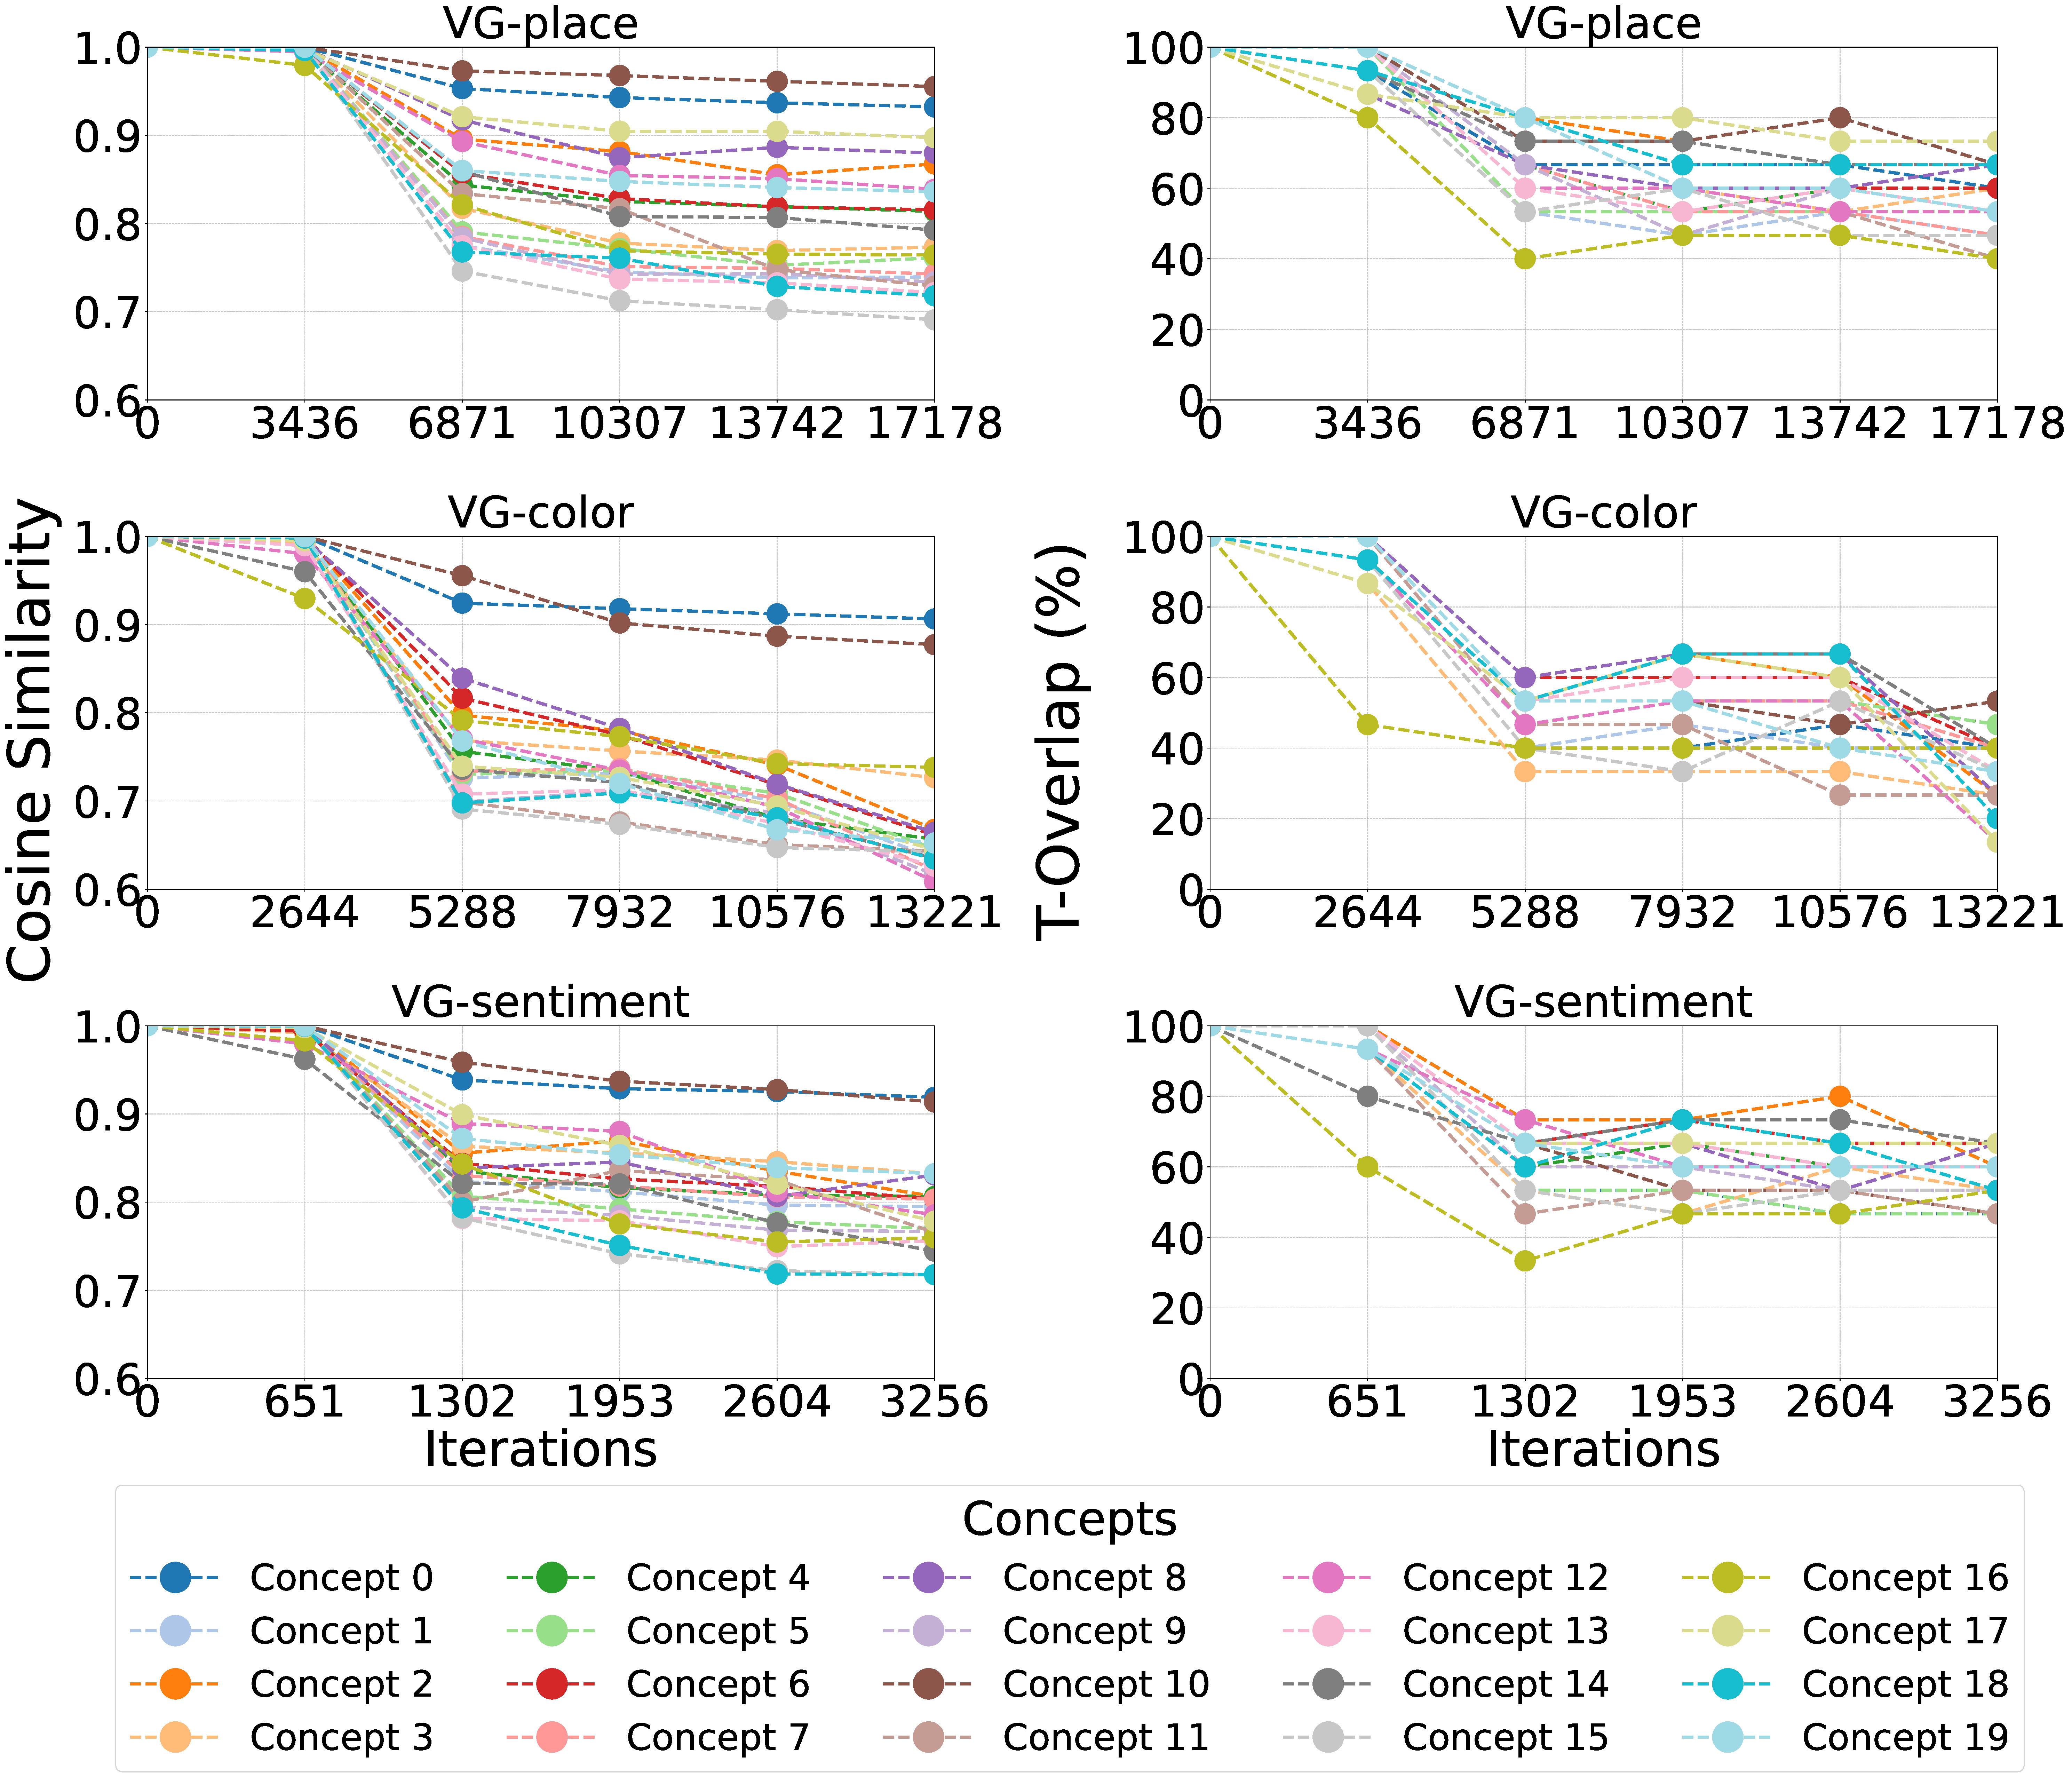
\includegraphics[width=\textwidth]{Figures/app/VG_dog_drift_cosine_sim_words_overlap_per_concept.pdf}}
        \label{fig:app_cosine_sim_text_overlap_per_concept}
    \end{minipage}
    



    \vspace{0.5cm}

    \begin{minipage}{0.45\textwidth}
        \centering
        {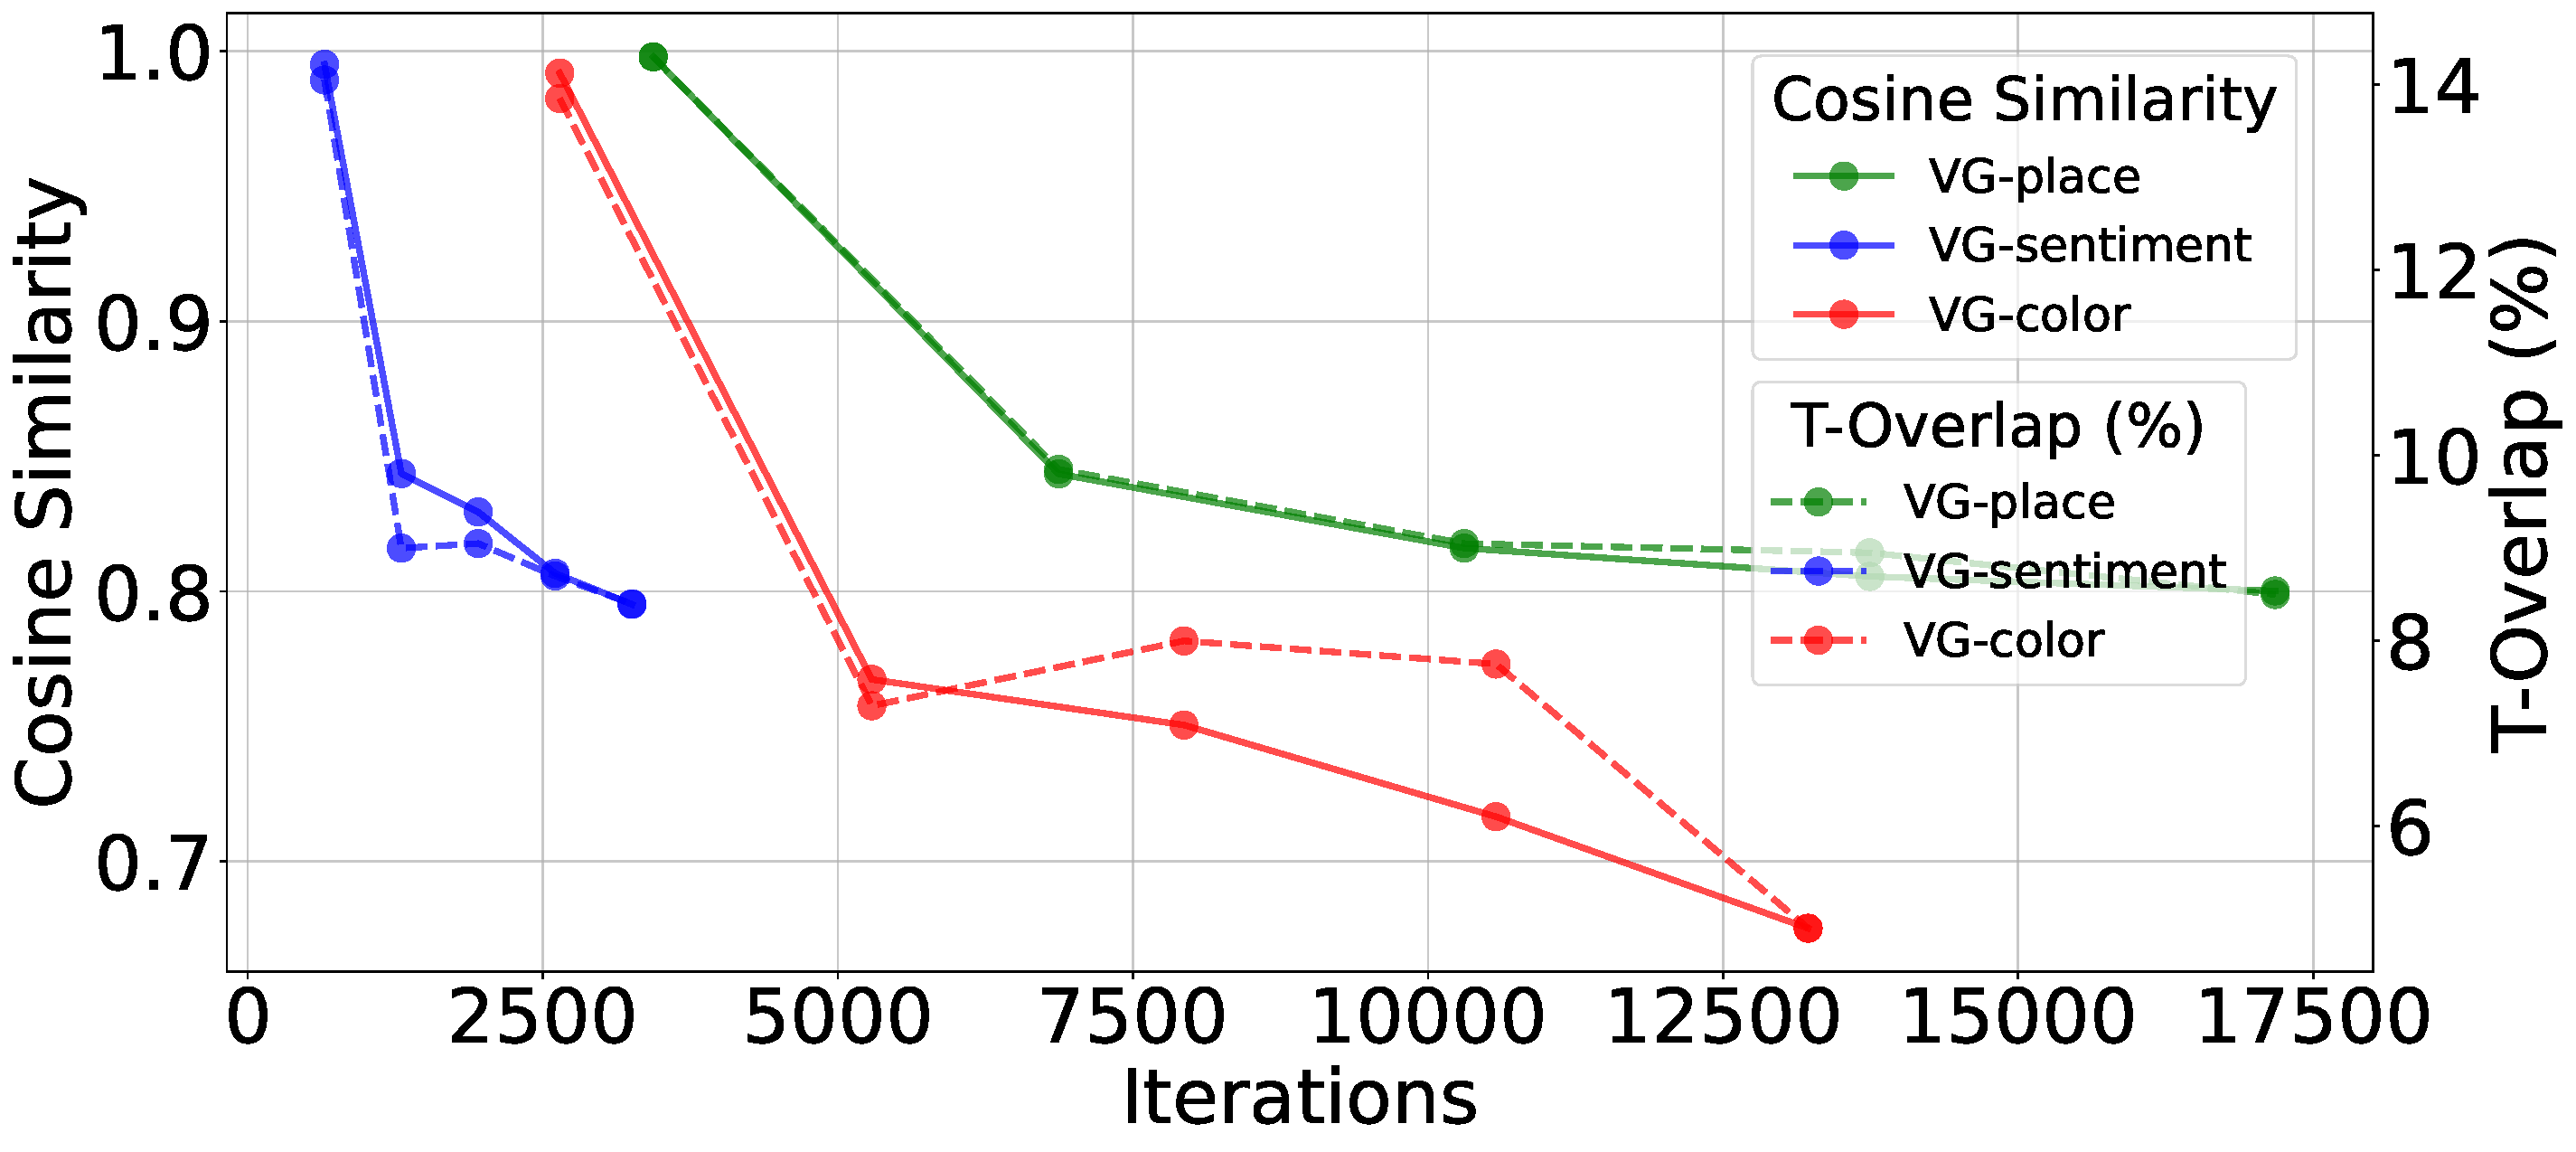
\includegraphics[width=\textwidth]{Figures/app/two_axes_cosine_words_intersection.pdf}}
        \label{fig:app_mean_cosine_sim_word_intersection_drift}
    \end{minipage}


    \caption{\textbf{Concepts change during training.} Illustration of the similarity between the original concepts the concepts during fine-tuning. Top: individual concepts change. Bottom: average concepts change.}
    \label{fig:concept_drift}
\end{figure}





\begin{figure*}[t]
    \centering
    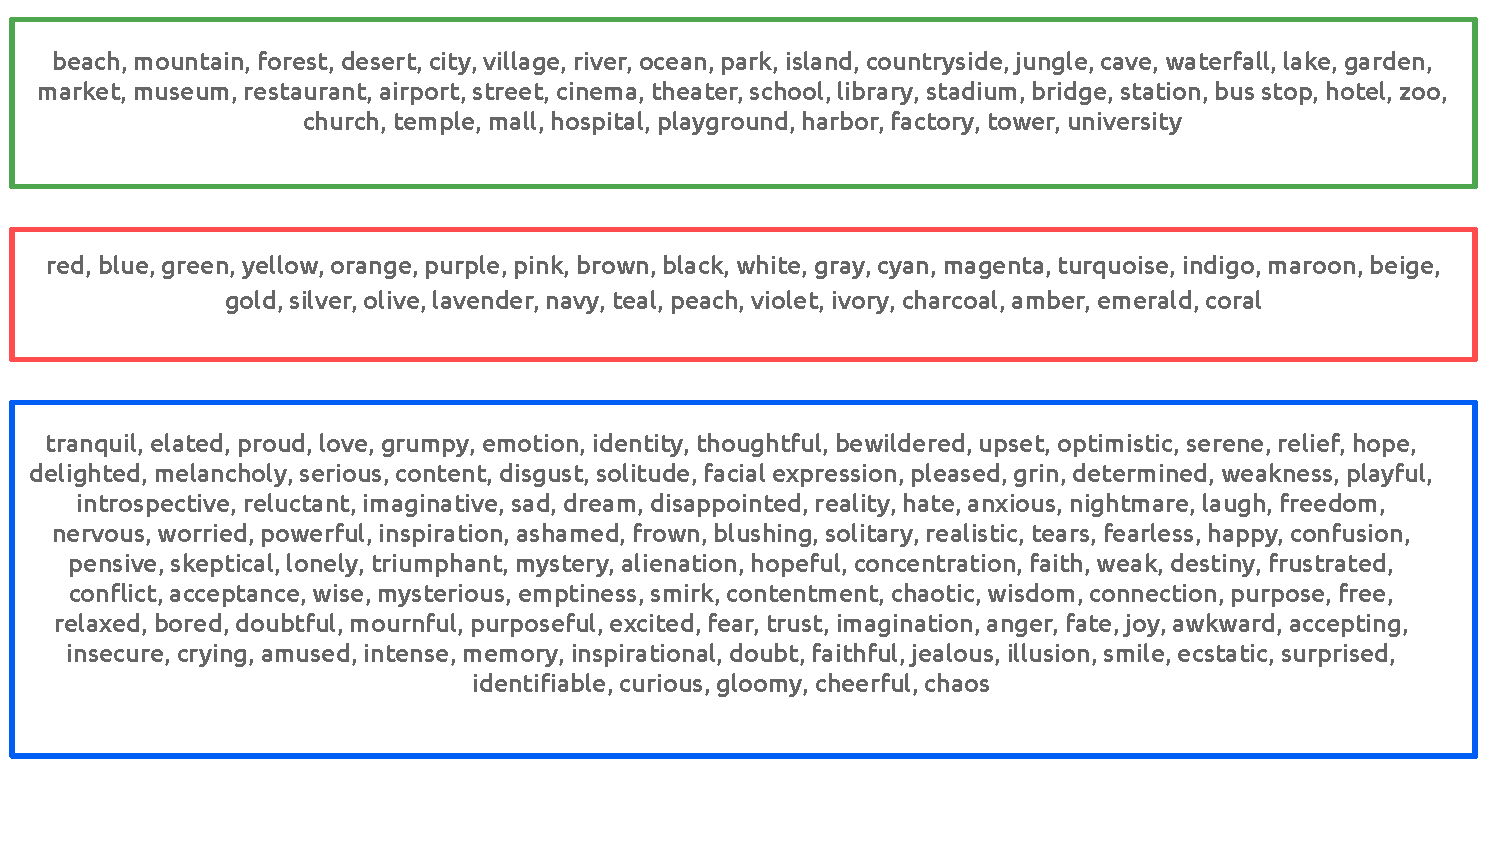
\includegraphics[width=1.0\linewidth]{Figures/app/training_words.pdf}
    \caption{\textbf{VG subsets.} Keywords used to extract VG subsets. Each subset is selected based on the presence of the corresponding words in the captions. From top to bottom, words related to: places, colors, and sentiments.}
    \label{fig:app_train_words}
\end{figure*}


\subsection{Concepts change during training}
\label{sec:app_4_concept_drift}

In this section, we show how fine-tuning deviates the fine-tuned concepts compared to the original ones.


To this end, we analyze the cosine similarity and text grounding overlap ($\text{T-Overlap}$) for each concept across training epochs and subsets. 
Specifically, we examine the cosine similarity and word overlap between an original concept $\bm{u}^a_{i}$ and its closest match $m(i)$ in the fine-tuned model at various stages of fine-tuning, where $m(i)$ is defined as:
\begin{align*}
& m(i) = \argmax_{\bm{u}^b_{j} \in \bm{U}^b} \text{cos}(\bm{u}^a_{i}, \bm{u}^b_{j})
\end{align*}


\Cref{fig:concept_drift} shows that both the cosine similarity and text overlap plots exhibit a consistent decreasing trend throughout fine-tuning, indicating that the model deviates further from the original concepts as training progresses. 

In the per-concept plot, we observe that the fine-tuning process affects each \textit{dog}-related concept differently, demonstrating various levels of change across concepts. Notably, concepts 0 and 10, which are related to \textit{hot dogs} rather than \textit{dogs}, exhibit a relatively smaller drift, suggesting that the fine-tuning process impacts different concepts with varying magnitudes. These results further support our observation that fine-tuning leads to a systematic deviation from the original model's representations, though the extent of this drift varies between concepts.















    


    
    



    












    



\begin{figure}[t]
    \centering
    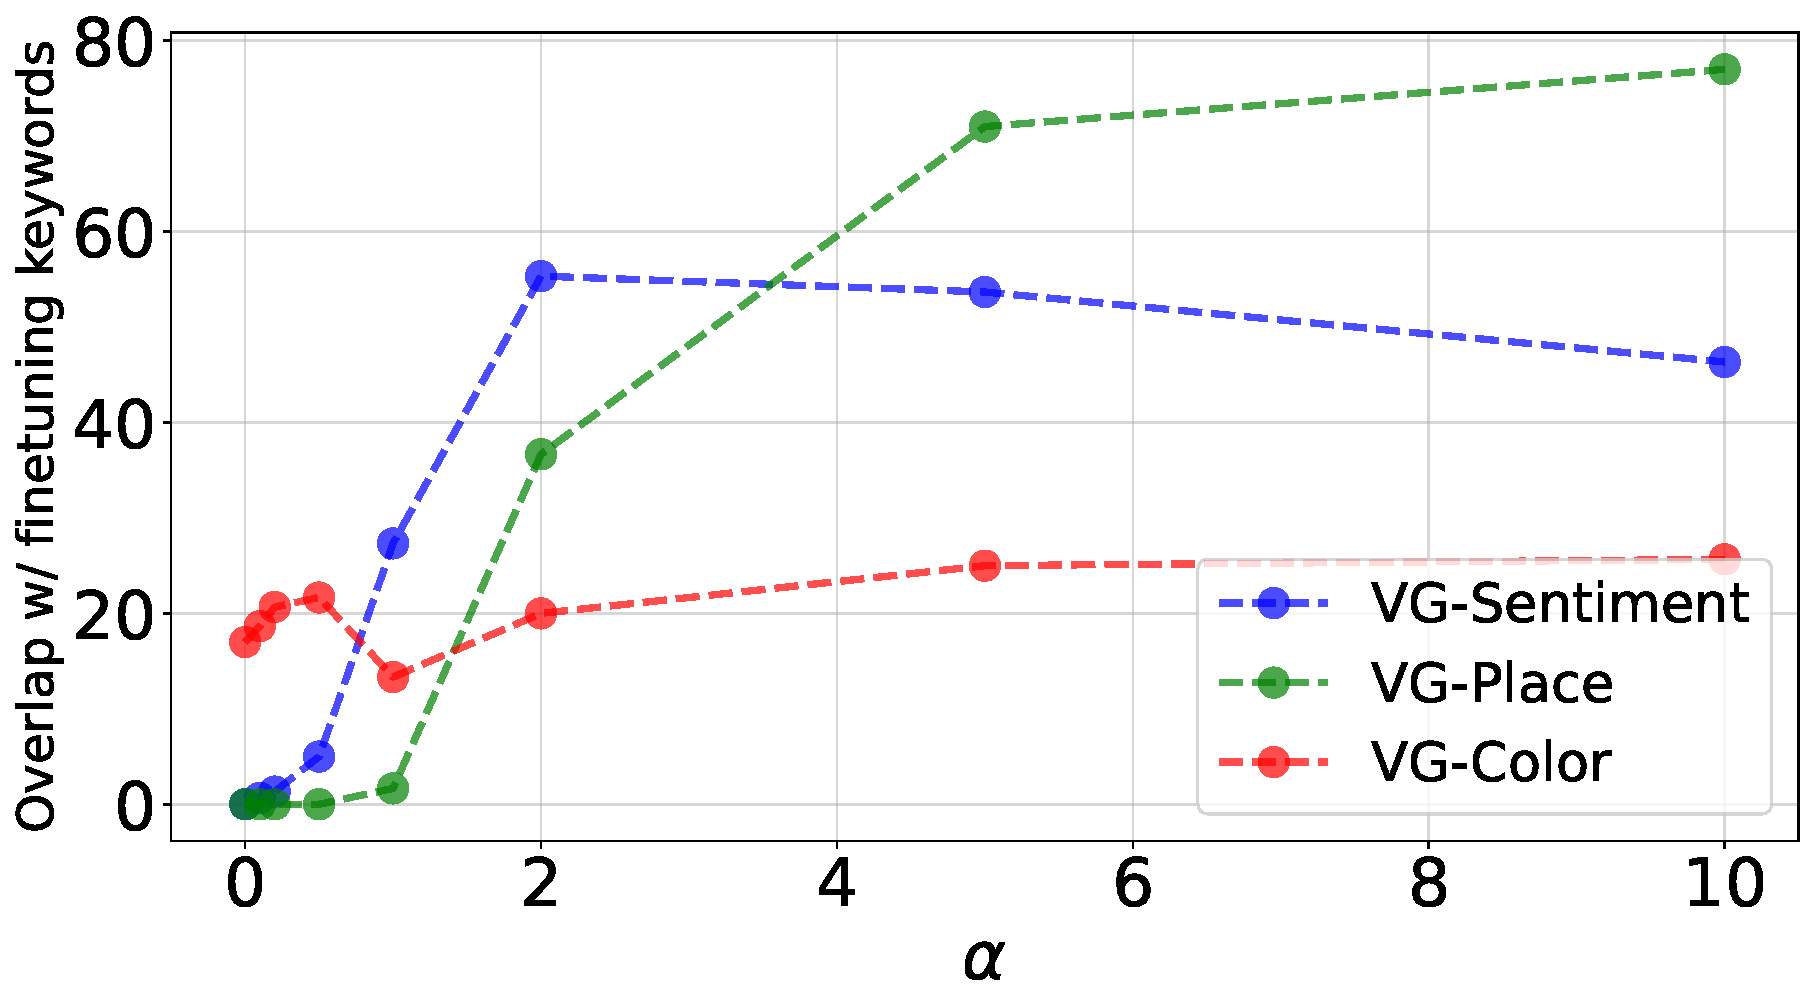
\includegraphics[width=0.99\linewidth]{Figures/intersection_keywords_mean.pdf}
    \caption{\textbf{Concepts specialization to the fine-tuning task.} Illustration of the mean intersection between the text grounding of shifted concepts (with magnitude $\alpha$) and the keywords associated with different fine-tuning datasets (with TOI `Dog'). $\alpha=0$ corresponds to the original model.}
    \label{fig:app_shift_keywords_intersection}
\end{figure}




\subsection{Concepts recovery and shift vectors}
\label{sec:app_4_concept_recovery}

\subsubsection{Concepts specialization to the fine-tuning task}
\label{sec:app_4_concept_shift_beyond}

We investigate the relationship between the shift vectors effect and the fine-tuning task. We vary $\alpha$ and report the average (average over $K=20$ concepts) overlap between the text grounding of the shifted concept $\bm{u}^s_k$ and the set of keywords $\{w_1, \ldots, w_m\} \subset \bmY$ associated with the fine-tuning task (Sec. 3). \Cref{fig:app_shift_keywords_intersection} shows that the shift vectors move the original clusters to be more related to the task keywords. 




\subsubsection{Ablation study}
\label{sec:app_recovery_ablation}

In the following, we present ablation studies to different design choices.


\paragraph{Number of concepts and recovery.}
We investigate the effect of varying the number of concepts $K$ on the recovery. We report the $\text{T-Overlap}$ between the fine-tuned model concepts and their match (matching is bijective as in \Cref{sec:app_bijective_matching_notation}), both in the shifted $\bm{u}^s_k$ and the original concepts $\bm{u}^a_k$. \Cref{fig:app_k_ablation_mas_words} shows that the number of concepts does not significantly influence the concept recovery.







\begin{figure}
    \centering
    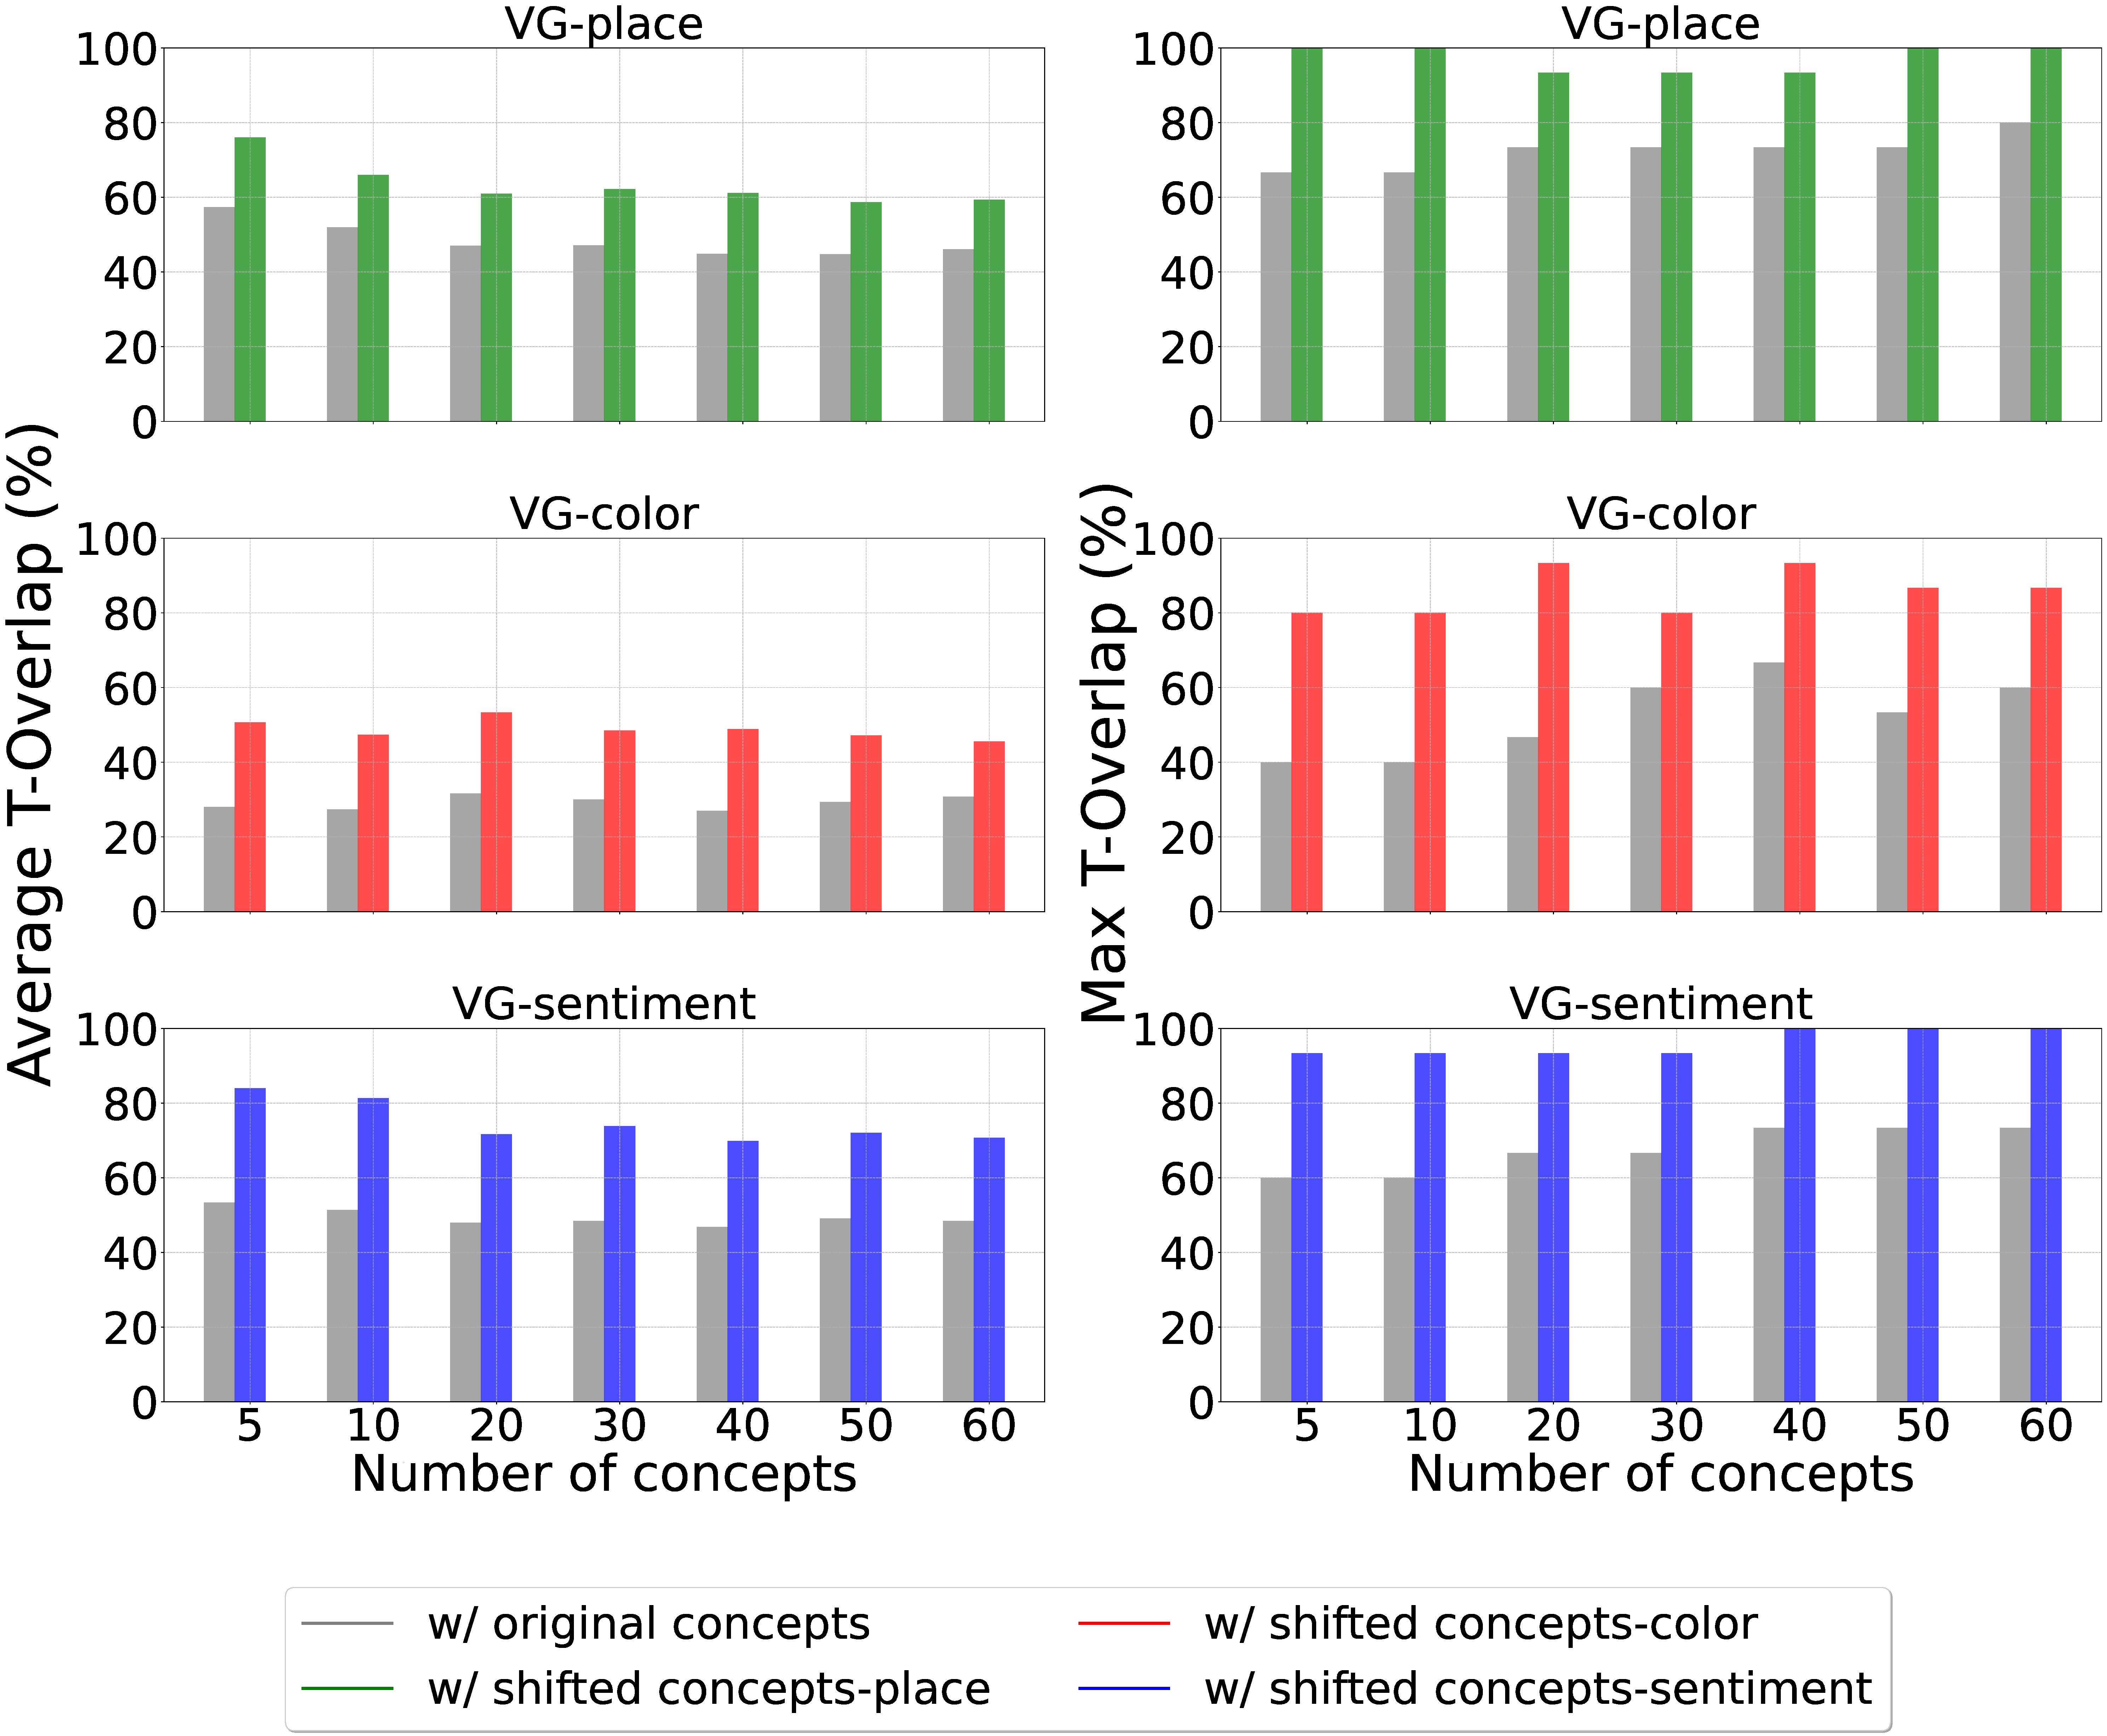
\includegraphics[width=1\linewidth]{Figures/app/VG_bars_coco_dog_grounding_recovery_words_k_ablation_average_and_max.pdf}
    \caption{\textbf{Concepts extraction layer and recovery.} We investigate the impact of shifting concepts extracted from different layers, and evaluate their recovery. The results show that the recovery improves with deeper layers, as the gap between the T-Overlap with original and with shifted concepts becomes larger.
    }
    \label{fig:app_k_ablation_mas_words}
\end{figure}






\paragraph{Concepts recovery across layers.} We investigate the effect of varying the layer from which we extract the concepts. We report the average and the maximum of $\text{T-Overlap}$. \Cref{fig:app_layer_ablation_mas_words} shows that the gap between the $\text{T-Overlap}$ with shifted and $\text{T-Overlap}$ with original concepts is higher in deeper layers, indicating better recovery. 

\begin{figure}[t]
    \centering
    \begin{minipage}{0.45\textwidth}
        \centering
        \subfloat[]{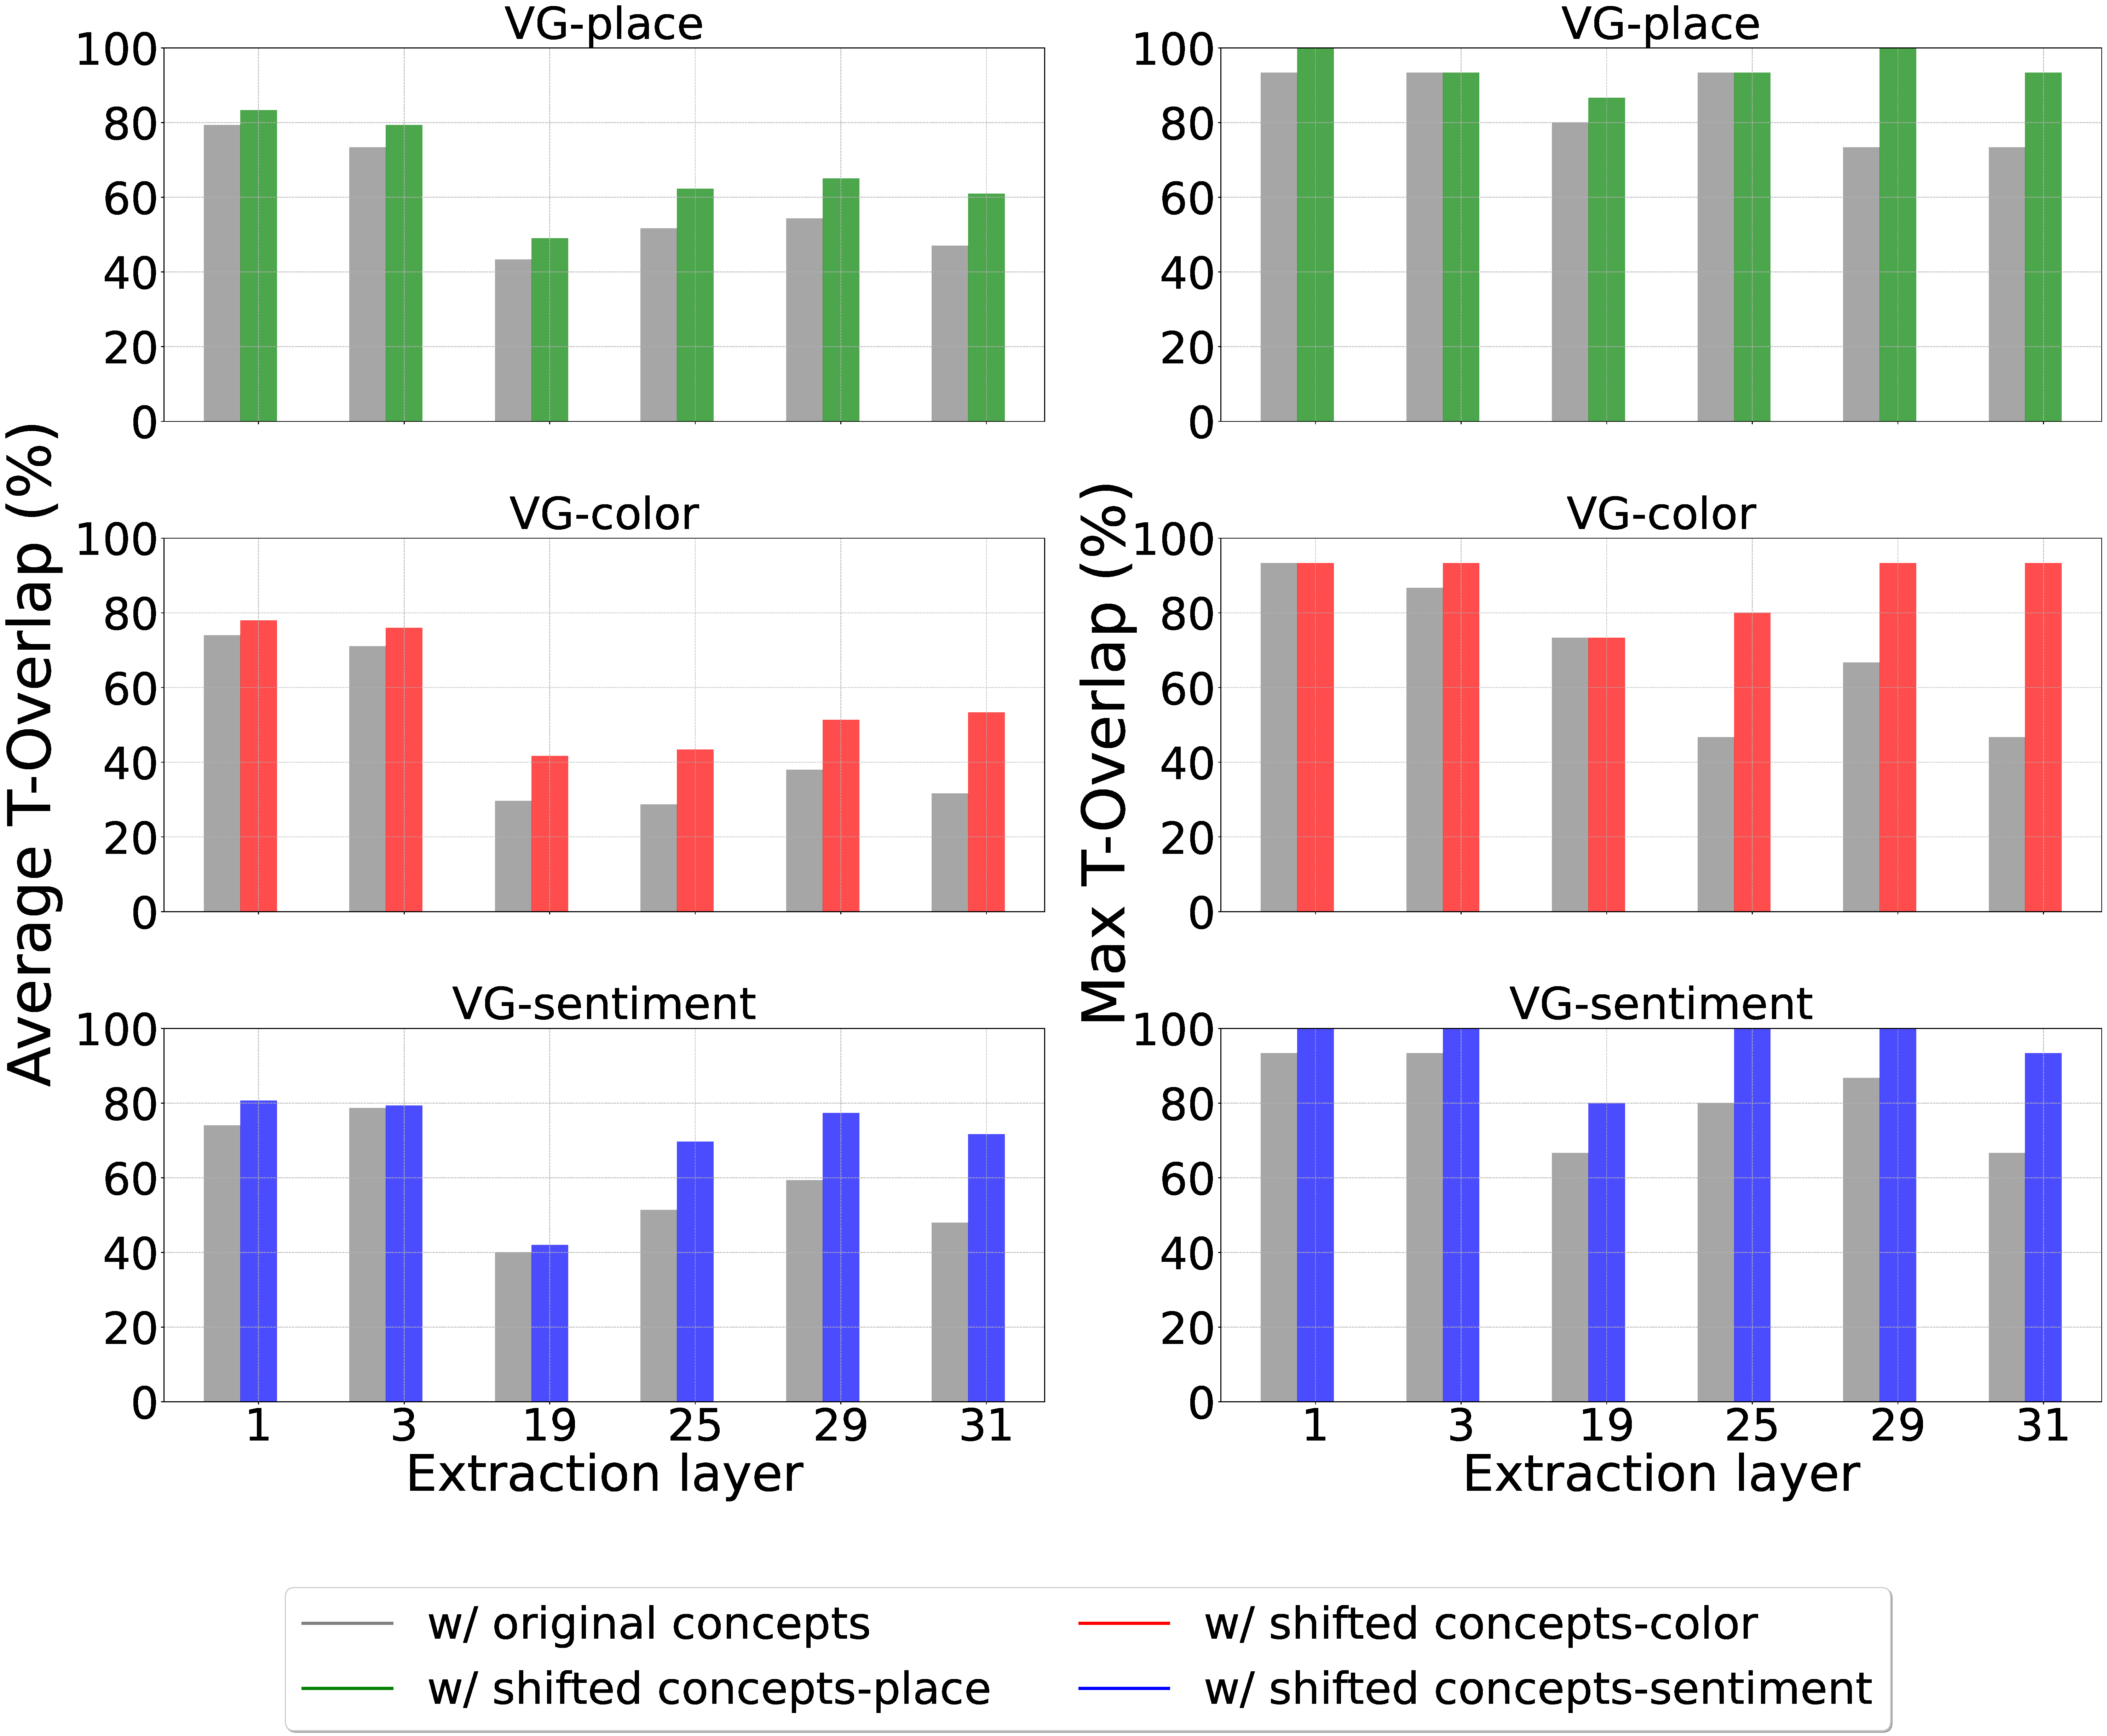
\includegraphics[width=\textwidth]{Figures/app/VG_bars_coco_dog_grounding_recovery_words_layer_ablation_average_and_max.pdf}}
        \label{fig:app_words_recovery_layer_ablation}
    \end{minipage}
    





    \caption{\textbf{Number of concepts and recovery.} Varying the number of concepts \(K\) has minimal impact on the recovery, as measured by the overlap metrics, indicating the robustness of the recovery process to the choice of \(K\).}
    \label{fig:app_layer_ablation_mas_words}
\end{figure}


















        
        
        
        








\subsection{Concepts shift consistency and magnitude}
\label{sec:app_consistency_correlation}





    
    







    


    











Each concept shift vector $\Delta^{a \to b}_k(\bm{u}^a_k)$ is computed from a set of individual sample representation shifts $\{\delta_m\}_{m \in \bm{A}_k}$. We hypothesize, that if the individual shifts are consistent (\emph{i.e.}, move in a single direction), the concept shift vector has a higher magnitude, which is highly correlated with the recovery of concepts. To this end, we quantify the consistency by computing the mean cosine similarity of individual representation shifts with the concept shift vector. This can be expressed using the cosine similarity between each vector \(\delta_m\) and the mean vector \(\bm{\Delta}_k^{a \to b}(\bm{u}^a_k)\):

    \[
    \text{Consistency}(\bm{u}_{k}^a) = \frac{1}{|\bm{A}_k|} \sum_{m \in \bm{A}_k} \text{cos}(\delta_m, \bm{\Delta}_k^{a \to b}(\bm{u}^a_k)),
    \]

We corroborate our hypothesis by plotting the variation of concept shift vector magnitudes with the consistency of their shifts for concepts related to animal dog in \Cref{fig:app_mag_mean_shift_shift_consistency}. Beyond the established correlation, the average magnitude of individual shifts $\delta_m$ remain similar across concepts ($48.06 \pm 3.887$, $57.6 \pm 1.796$, and $47.9 \pm 3.96$)— where the values represent the mean and standard deviation for animal dog concepts for different finetuning tasks. This suggests that a higher consistency is linked to a larger magnitude of the mean shift vector, indicating that individual shifts are more aligned and do not cancel each other out. \newline
We provide additional results using LLaVA model in \Cref{fig:app_llava_correlations}. 






    
    

    


    

    
    


















    



    



    



    








    

    

    
    












\begin{figure}[t]
    \centering
    \begin{minipage}{0.45\textwidth}
        \centering
        {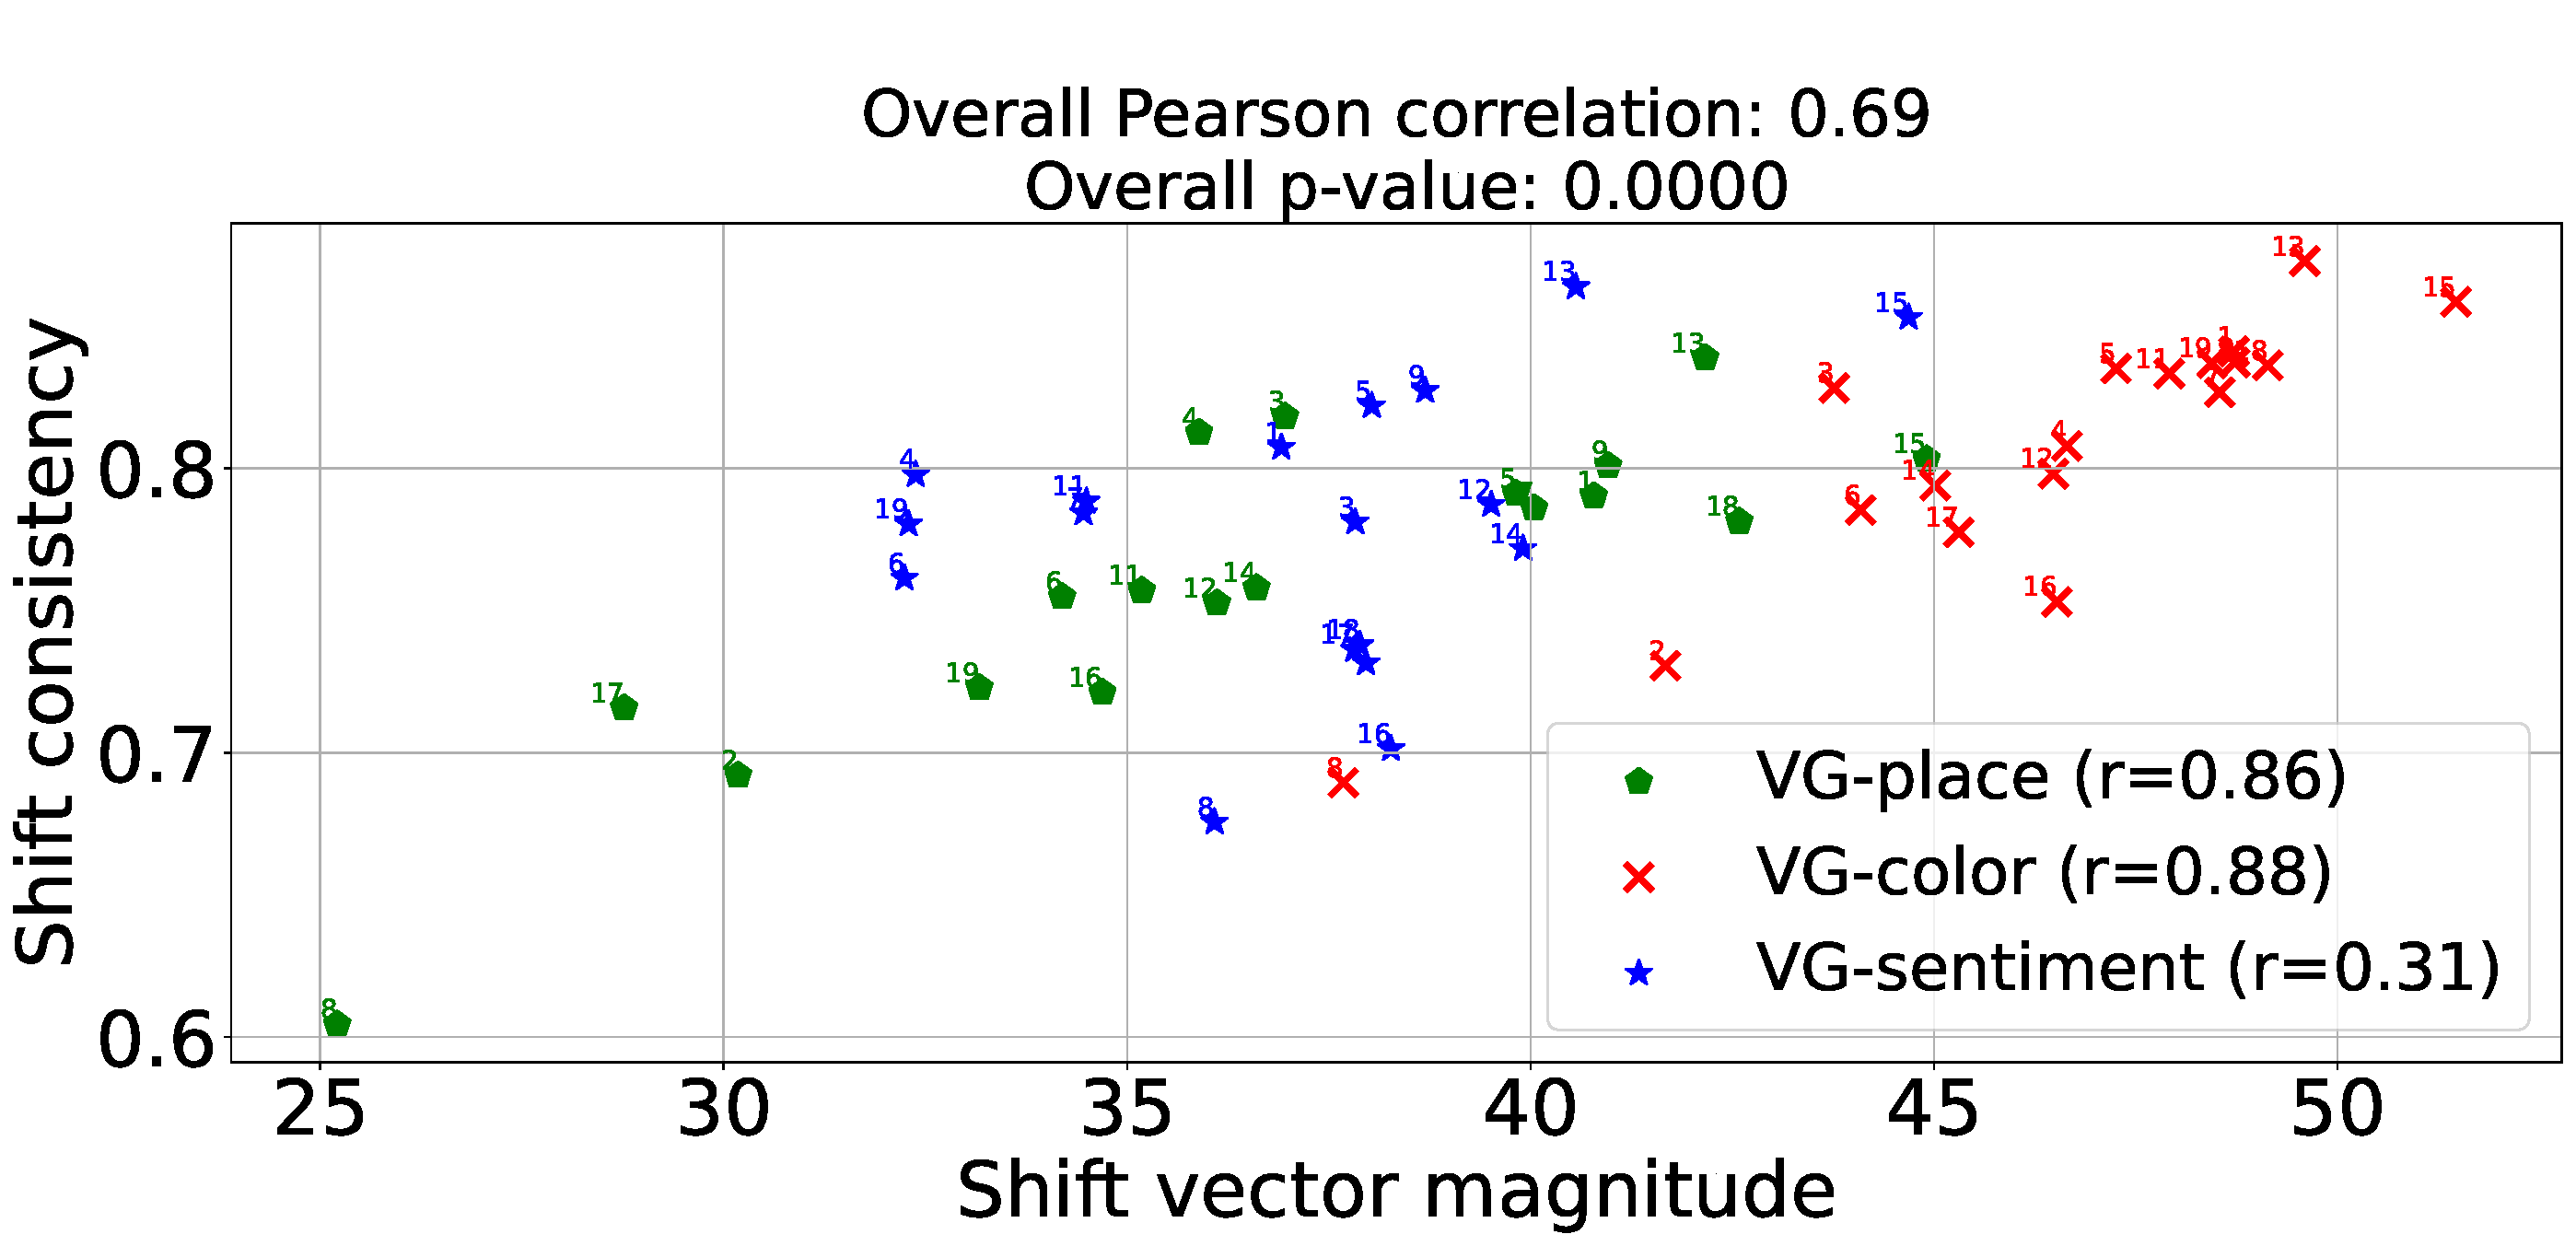
\includegraphics[width=\textwidth]{Figures/app/dog_mag_mean_shift_shift_consistency.pdf}}
        \label{fig:app_mag_mean_shift_shift_consistency}
    \end{minipage}

    \caption{\textbf{Correlation between the shift vector magnitude and the shift consistency.} Each point corresponds to a concept fine-tuned on 3 VG subsets. The higher the shift vector magnitude, the higher the shift consistency (as defined in \Cref{sec:app_consistency_correlation}) 
    }
    \label{fig:consistency_and_magnitude}
\end{figure}





















        

            

\subsection{Additional experiments with LLaVA model}
\label{sec:app_llava_experiments}
In this section, we extend our main experiments to the LLaVA model, adhering to the same experimental setup as described previously. We report the text grounding recovery evaluation in \Cref{fig:app_llava_word_recovery} and the relationship between shift metrics and the recovery in \Cref{fig:app_llava_correlations}, providing further insights into the consistency and generalizability of our findings across different models.
 








\begin{figure}
    \centering
    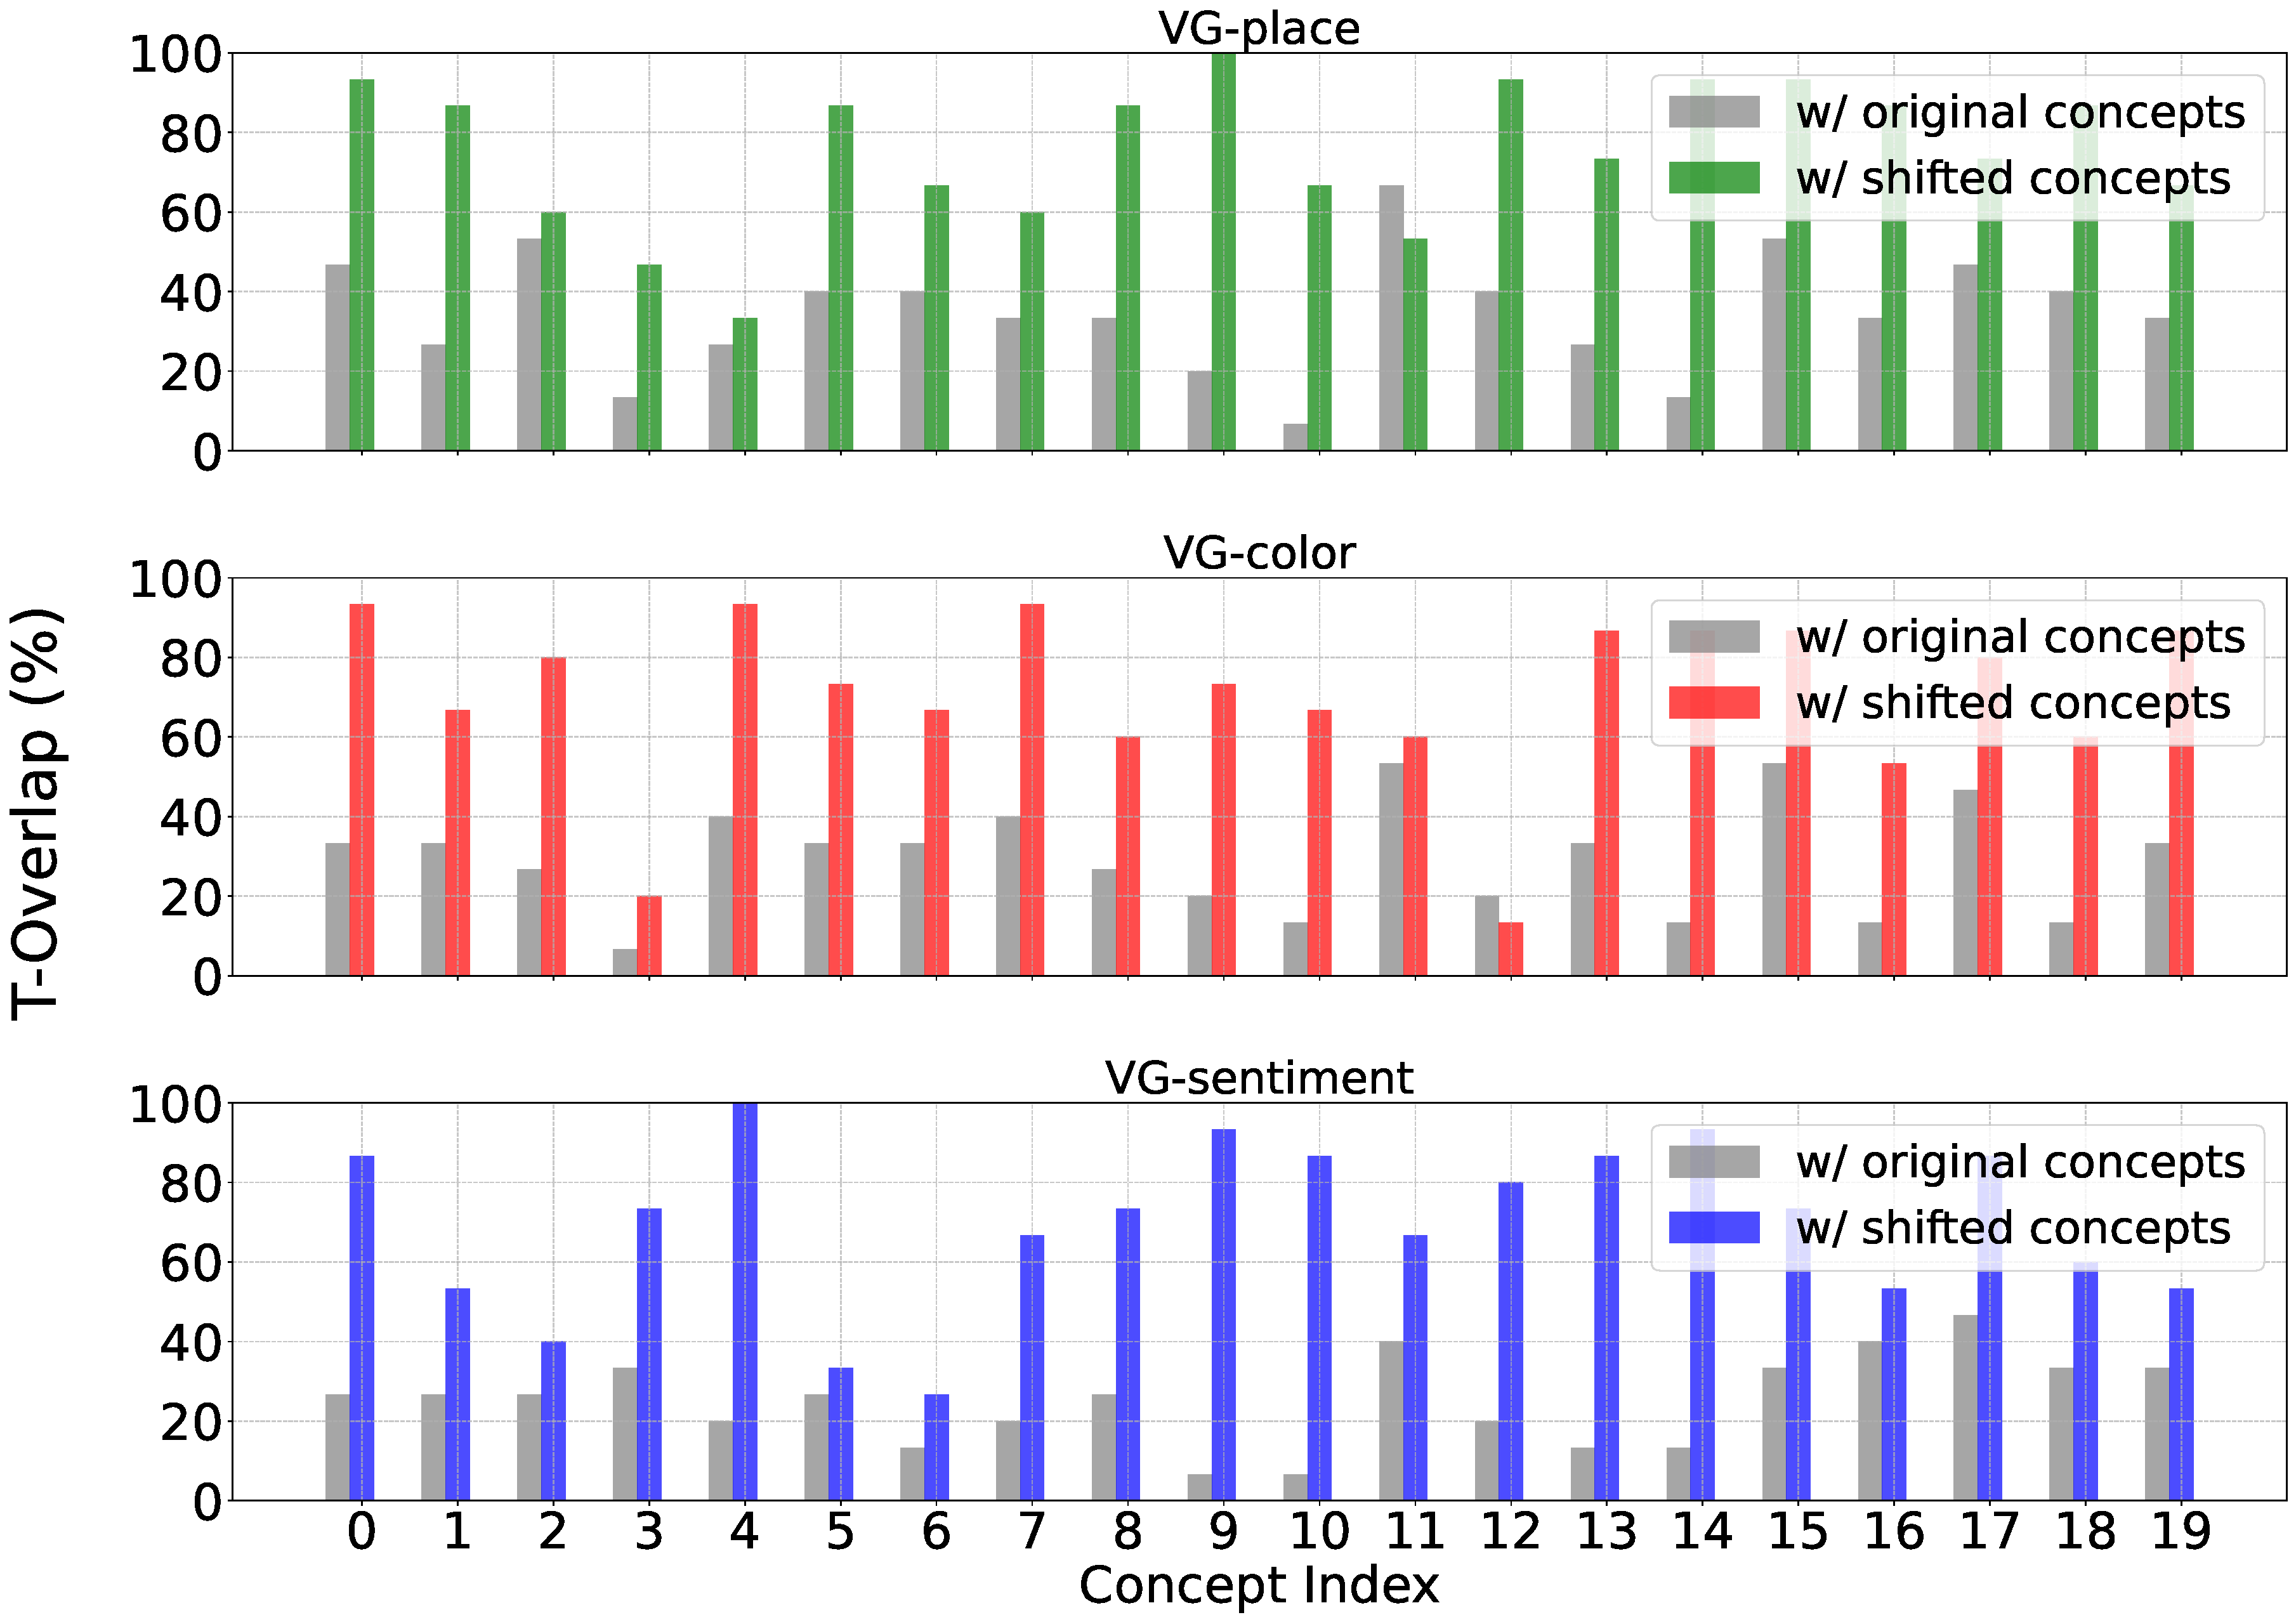
\includegraphics[width=1\linewidth]{Figures/app/VG_llava_bars_coco_dog_grounding_recovery_words.pdf}
    \caption{\textbf{Recovering fine-tuned LLaVA-1.5 model concepts.} For each matched fine-tuned concept we report its text grounding overlap with the original concept and the shifted concept. Model fine-tuned on: places (top), colors (middle) and sentiments (bottom).}
    \label{fig:app_llava_word_recovery}
\end{figure}


\begin{figure}[t]
    \centering
    \begin{minipage}{0.45\textwidth}
        \centering
        \subfloat[\textbf{Correlation between shift vector magnitudes and concept recovery for LLaVA-1.5 model.} The higher the shift vector magnitude the better the concept recovery.]{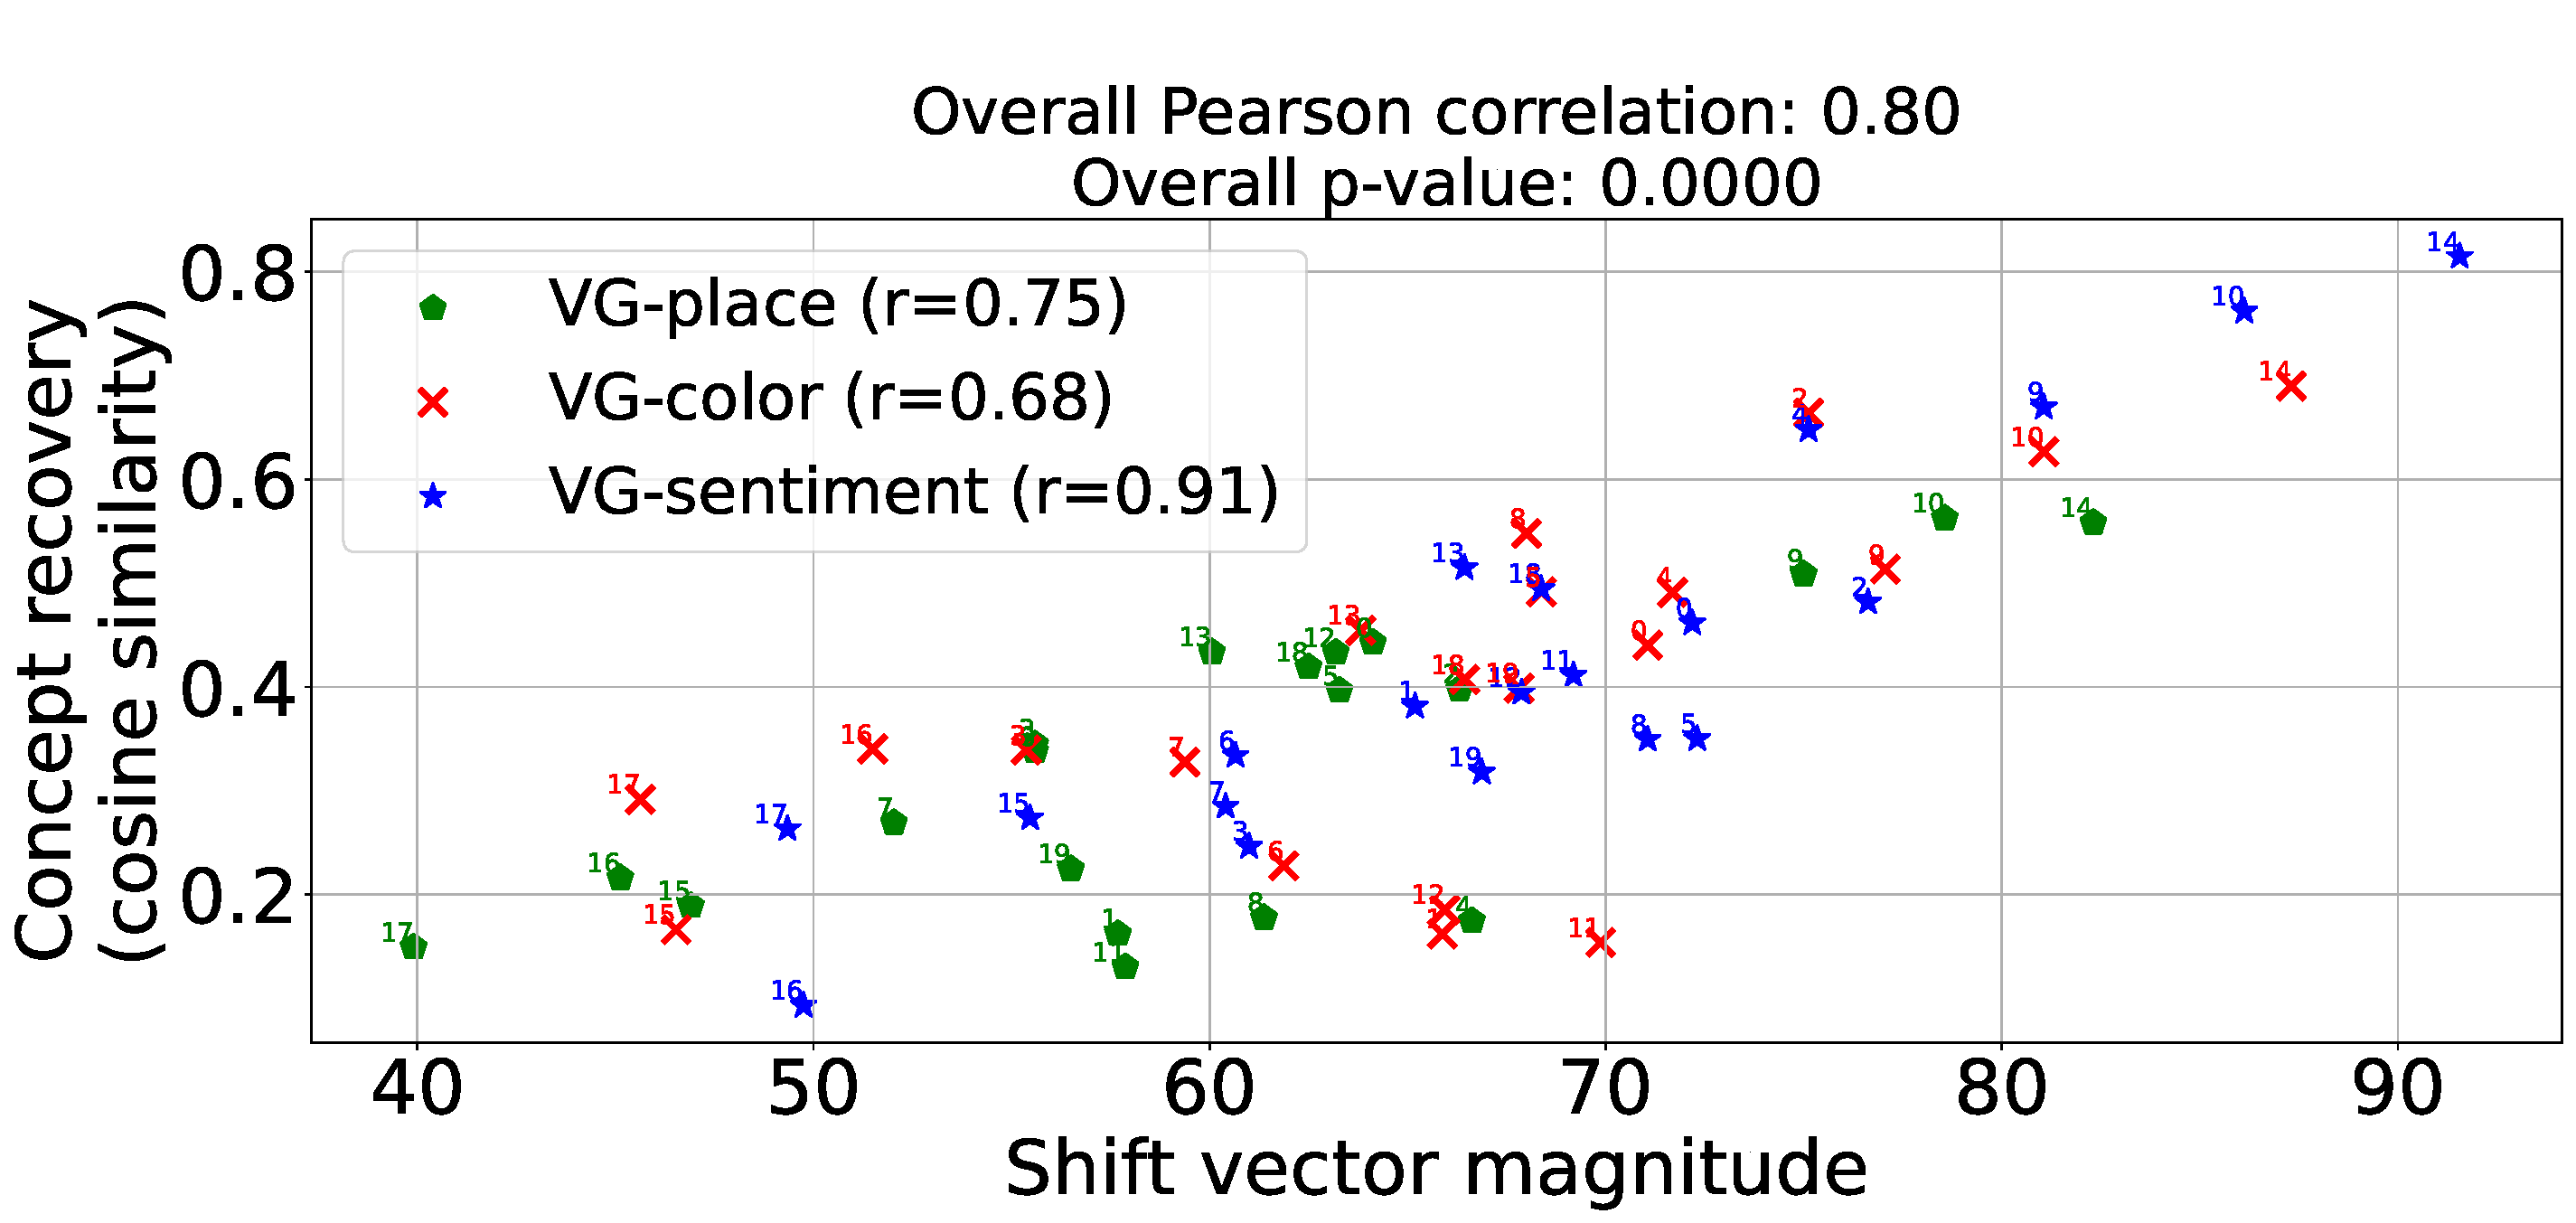
\includegraphics[width=\textwidth]{Figures/app/llava_dog_mag_mean_shift_cosine_improve_v2.pdf}}
        \label{fig:llava_mag_mean_shift_cosine_improve_v2}
    \end{minipage}

    \begin{minipage}{0.45\textwidth}
        \centering
        \subfloat[\textbf{Correlation between the shift vector magnitude and shift consistency.} The higher the shift vector magnitude, the higher the shift consistency.]{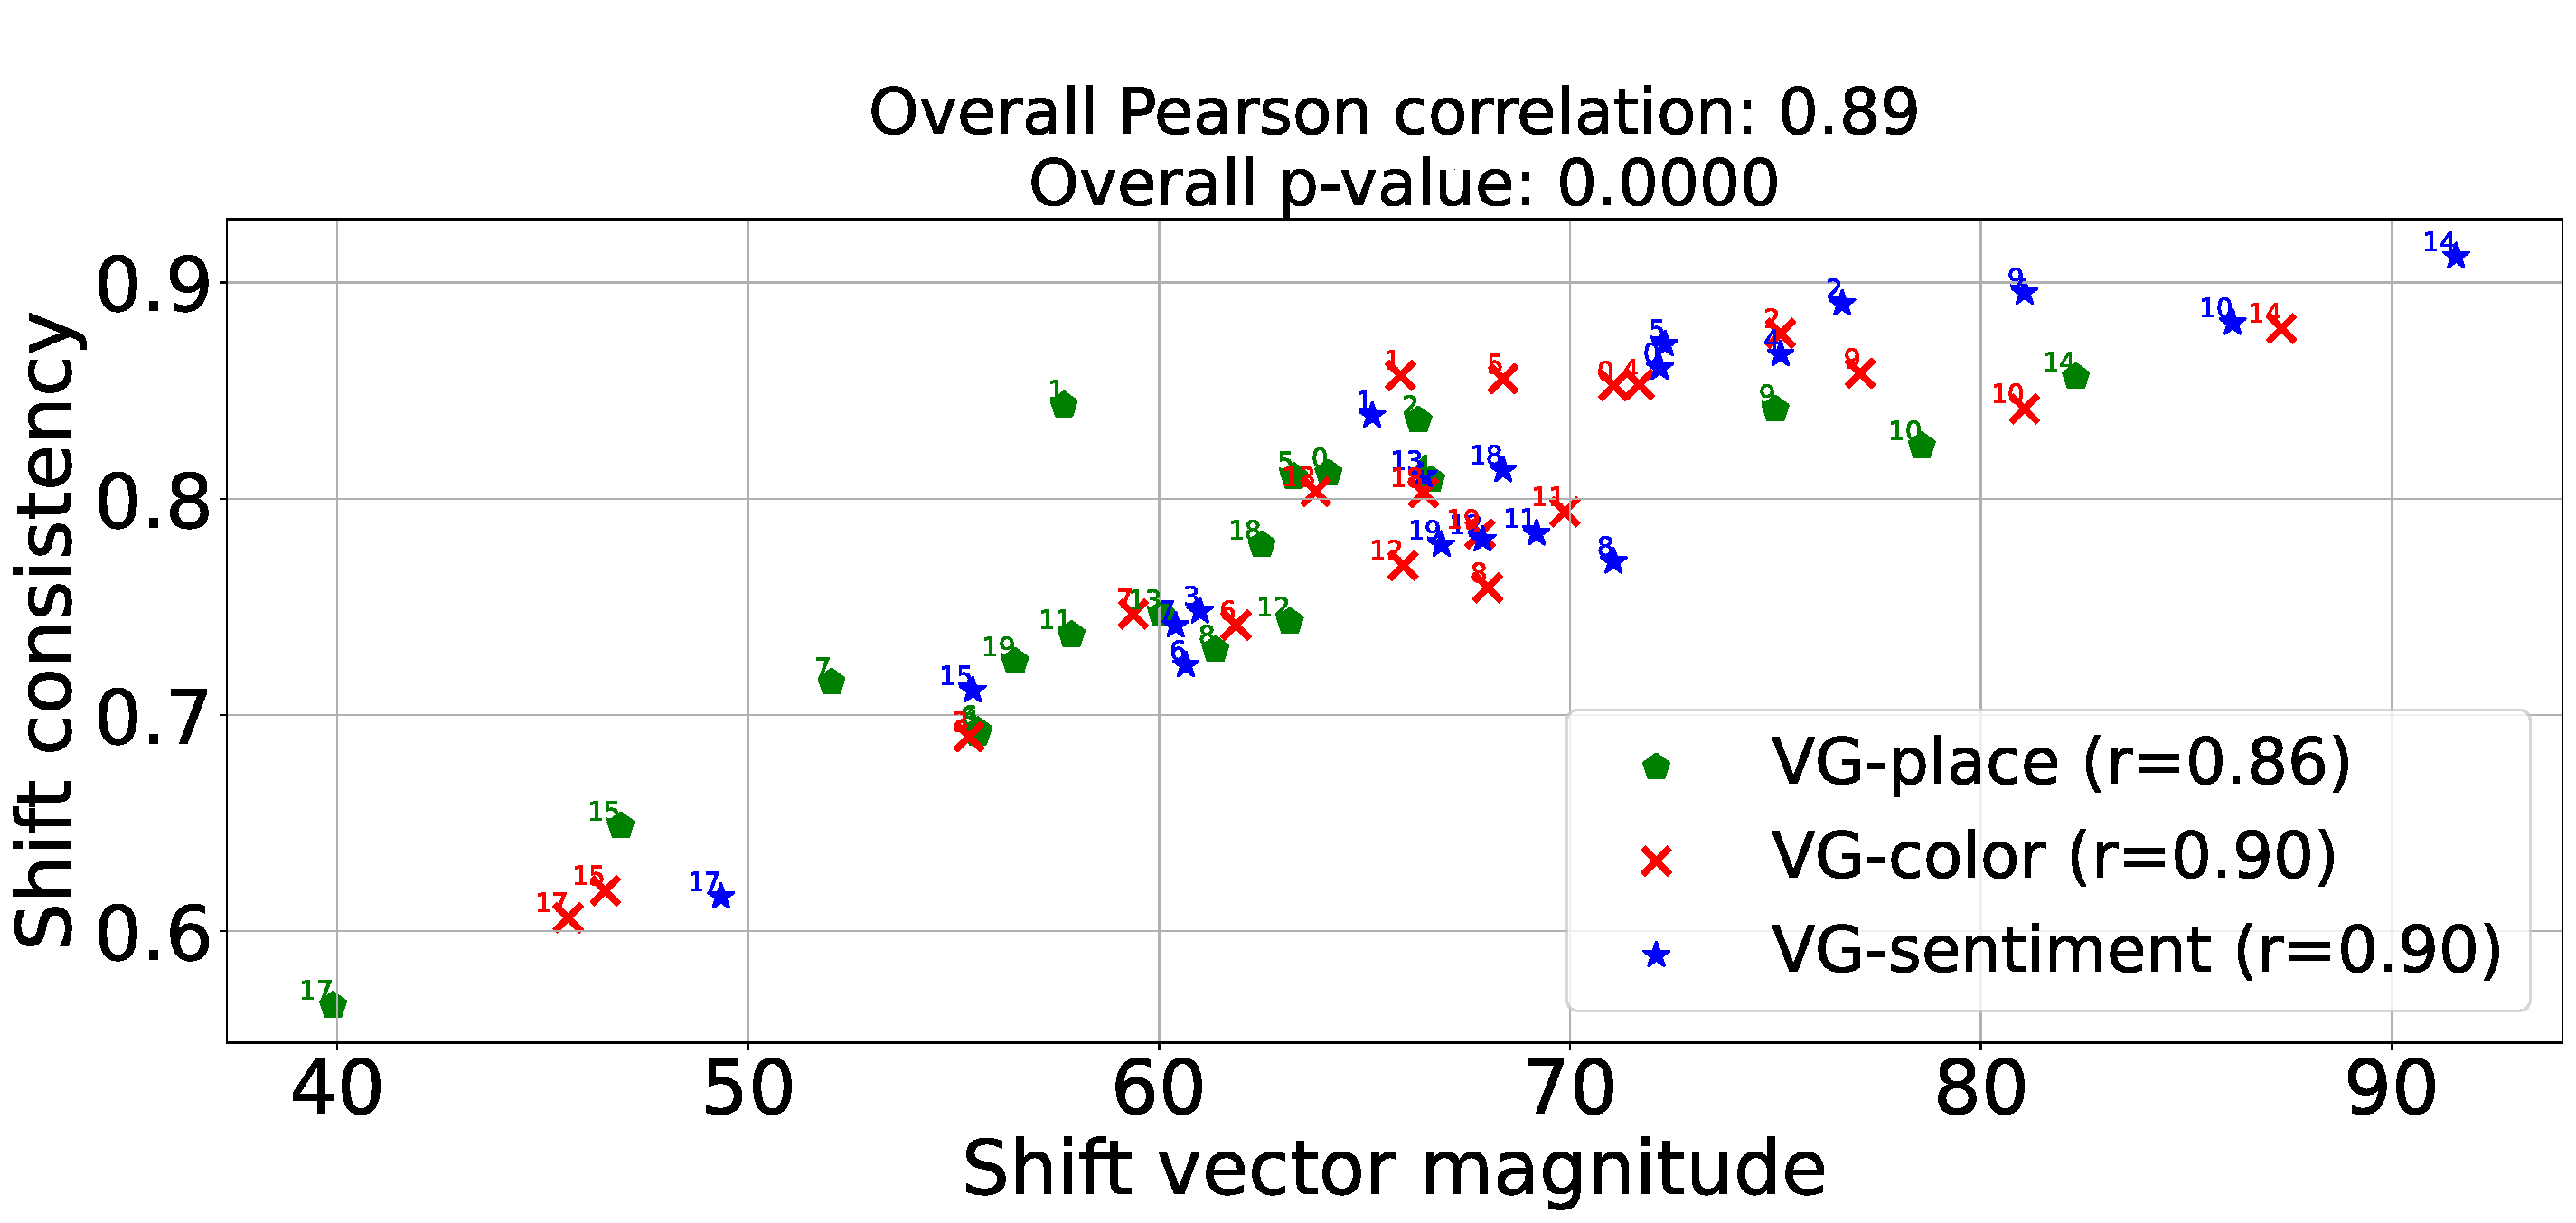
\includegraphics[width=\textwidth]{Figures/app/llava_dog_mag_mean_shift_shift_consistency.pdf}}
        \label{fig:app_llava_mag_mean_shift_shift_consistency}
    \end{minipage}


    \caption{\textbf{Concepts recovery and shift consistency with LLaVA-1.5.} Each point corresponds to a concept from LLaVA-1.5 fine-tuned on 3 VG subsets. Beyond the established correlation, the similar magnitude of individual shifts across concepts ($80.3 \pm 7.086$, $84.1 \pm 6.31$, and $85.6 \pm 5.95$)—where the values represent the mean and standard deviation of averaged individual shift magnitudes across animal dog concepts-suggests that a higher consistency is linked to a larger magnitude of the mean shift vector, indicating that individual shifts are more aligned and do not cancel each other out.}
    \label{fig:app_llava_correlations}
\end{figure}








\section{Fine-grained multimodal LLM steering}
\label{sec:app_model_steering}


This section provides additional results and details about model steering. Specifically, implementation details \Cref{sec:app_model_steering_implem_detail}, discovering steering directions towards single or multiple concepts \Cref{sec:app_model_steering_discover_concepts}, steering image captions \Cref{sec:app_image_captions}, ablation study for the steering layer, number of samples and the steering strength \Cref{sec:app_model_steering_ablation_study}, more visualization related to the linear separability of concepts \Cref{sec:app_linear_sep}, and finally, some qualitative results \Cref{sec:app_model_steering_qual}. 

\subsection{Implementation details}
\label{sec:app_model_steering_implem_detail}



Experiments are conducted on the widely-used LLaVA model \cite{liu2024improvedllava}, comprising a CLIP image encoder, a two-layer MLP connector, and a 7B Vicuna-1.5 LLM. In the main paper, we focus on VQAv2 dataset \cite{goyal2017makingvqav2}, a visual question-answering corpus with image-question-answer triplets and annotated answer types ("yes/no", "number", and "other"). We provide also experiments on COCO captioning \cite{lin2014microsoft}, that contains images and captions describing them. Because COCO does not contain style annotations, we automatically annotate the dataset. Specifically, for each style (\emph{e.g.}, colors, places, sentiments) if any of the descriptive keywords (\emph{e.g.} red, blue, white ... for colors) is present in the caption, we consider it belonging to the corresponding style.
Steering vectors are derived from a subset of the training set, with model performance evaluated on the validation set. We only use few hundred examples to compute the steering vectors, as we find this design choice does not have a significant effect on the final results (\Cref{sec:app_model_steering_ablate_num_samples}). We did an ablation over the which layer to apply the steering and select the best layer based on an evaluation on a validation set (\Cref{sec:app_ablate_layers}). Specifically, for VQAv2 we find the last layer works best, while for COCO the 20th layer is best. We report the evaluation metrics (\emph{e.g.} accuracy, CIDEr) on 5k and 3k random samples for VQAv2 and COCO respectively.




\begin{figure}[!h]
    \centering
    \begin{minipage}{1\linewidth}
    \centering
        \begin{minipage}{\linewidth}
            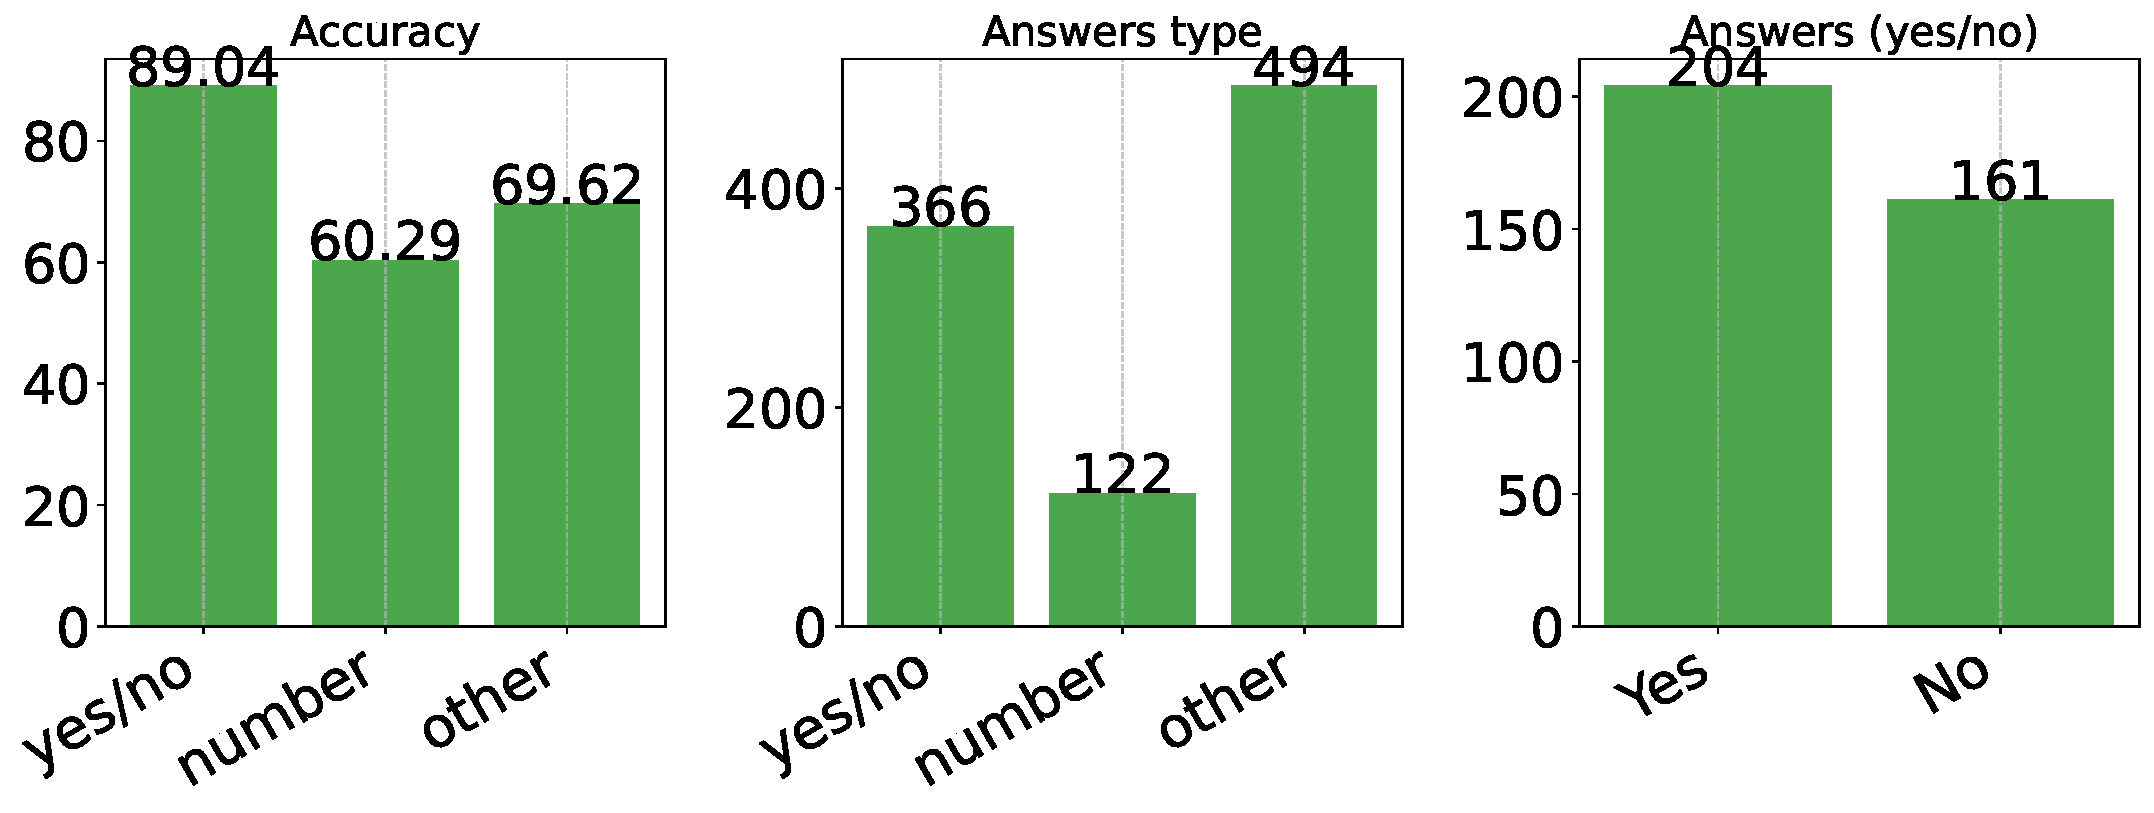
\includegraphics[width=1\textwidth]{Figures/model_steering/intra/steering_vector_vqav2_accuracy_llava_baseline_only_target_answers.pdf}
        \end{minipage}%
        
        \begin{minipage}{\linewidth}
            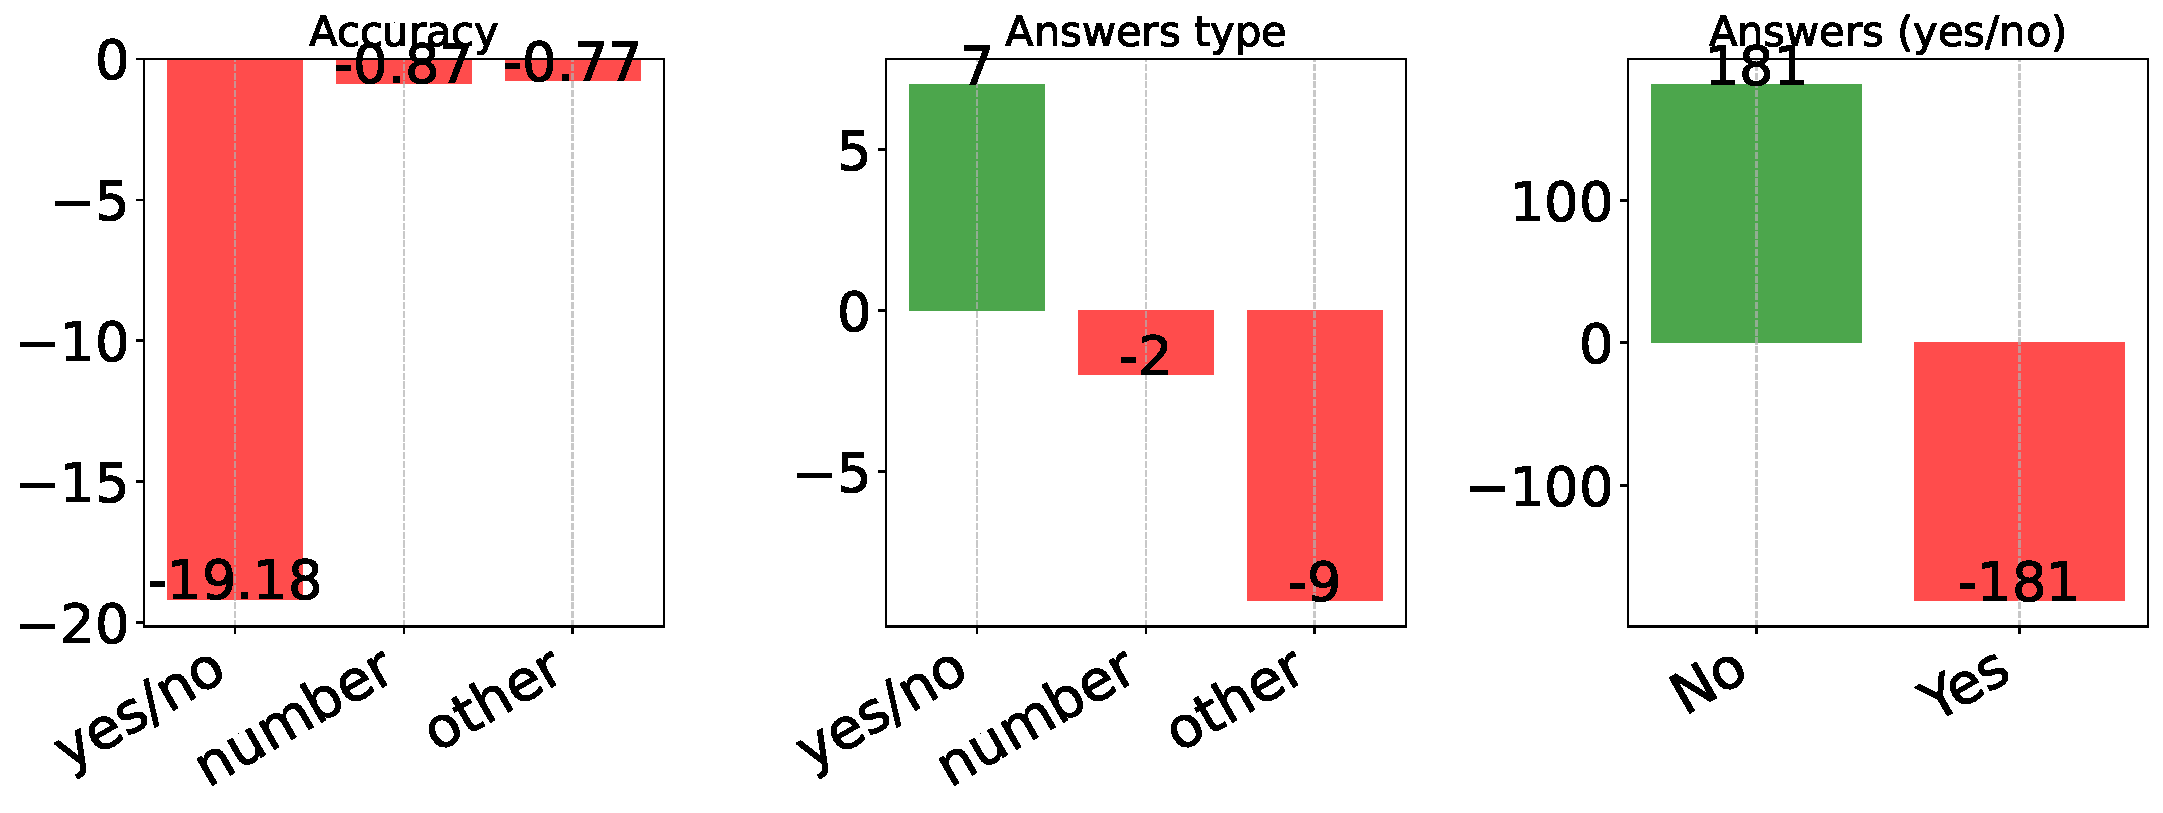
\includegraphics[width=1.0\textwidth]{Figures/model_steering/intra/steering_vector_vqav2_accuracy_llava_type_yes_no_steering_vector_concept_0_to_1_only_target_answers.pdf}
        \end{minipage}%
        
        \begin{minipage}{\linewidth}
            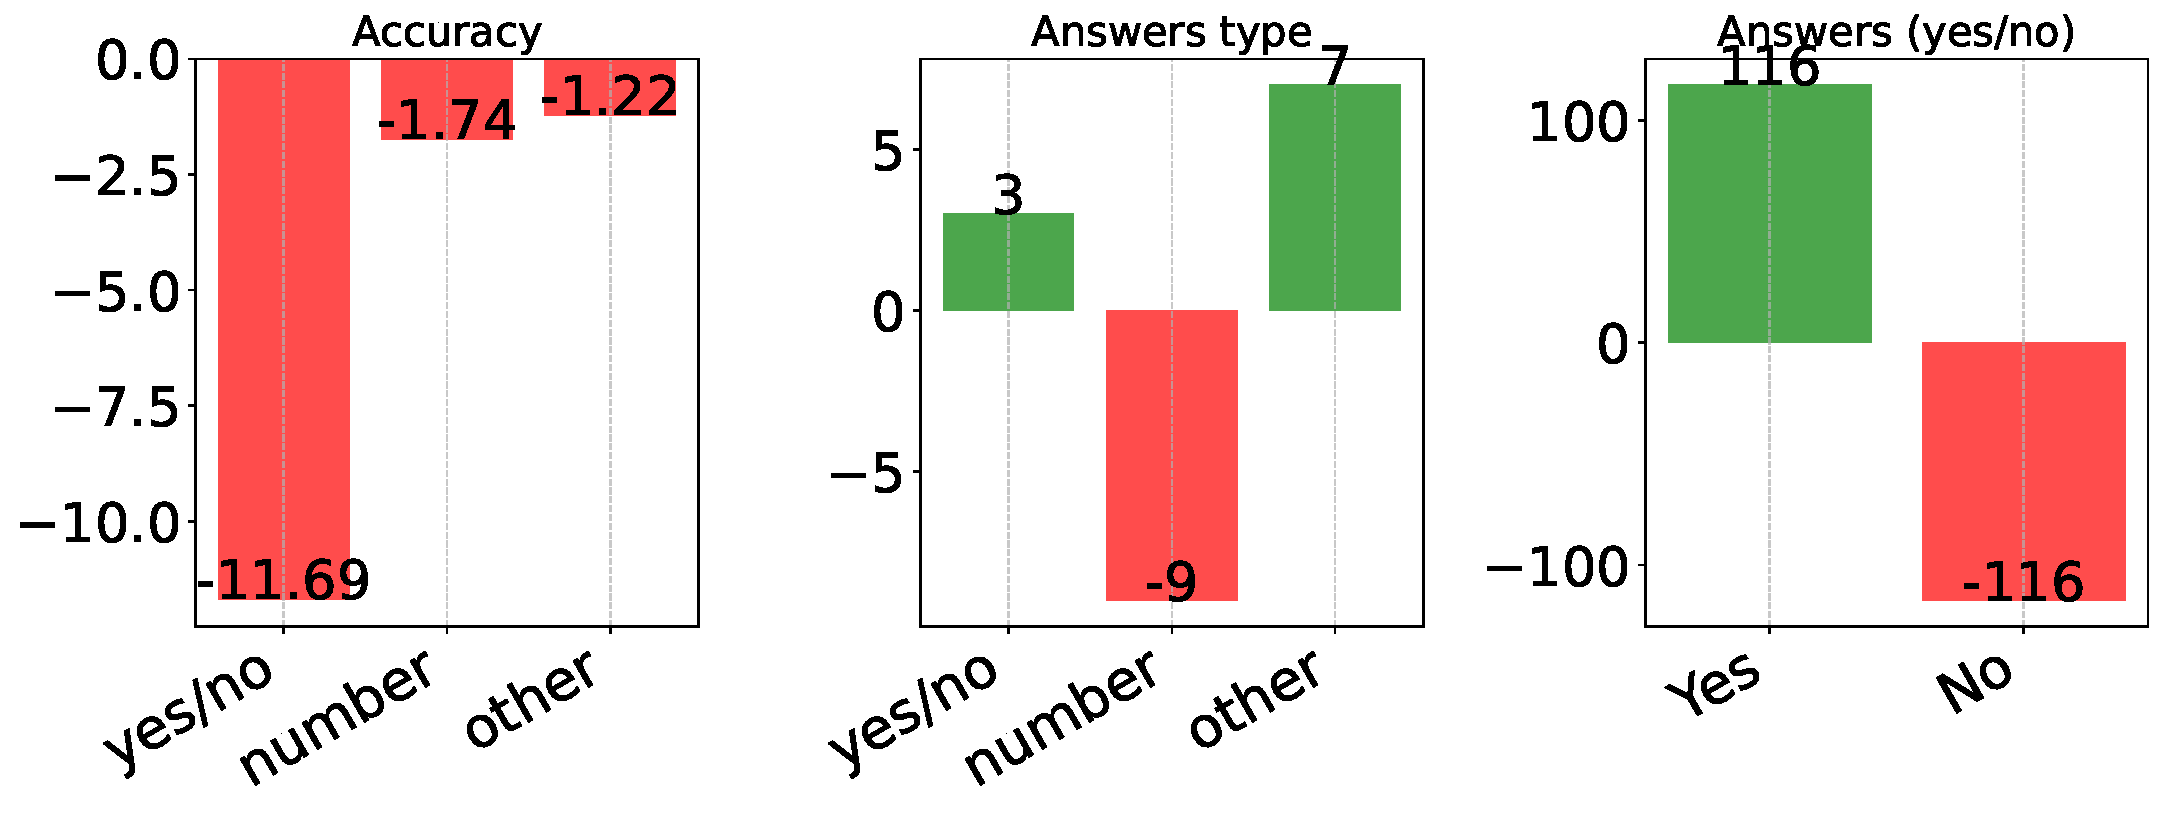
\includegraphics[width=1.0\textwidth]{Figures/model_steering/intra/steering_vector_vqav2_accuracy_llava_type_yes_no_steering_vector_concept_1_to_2_only_target_answers.pdf}
        \end{minipage}%
        
        \begin{minipage}{\linewidth}
            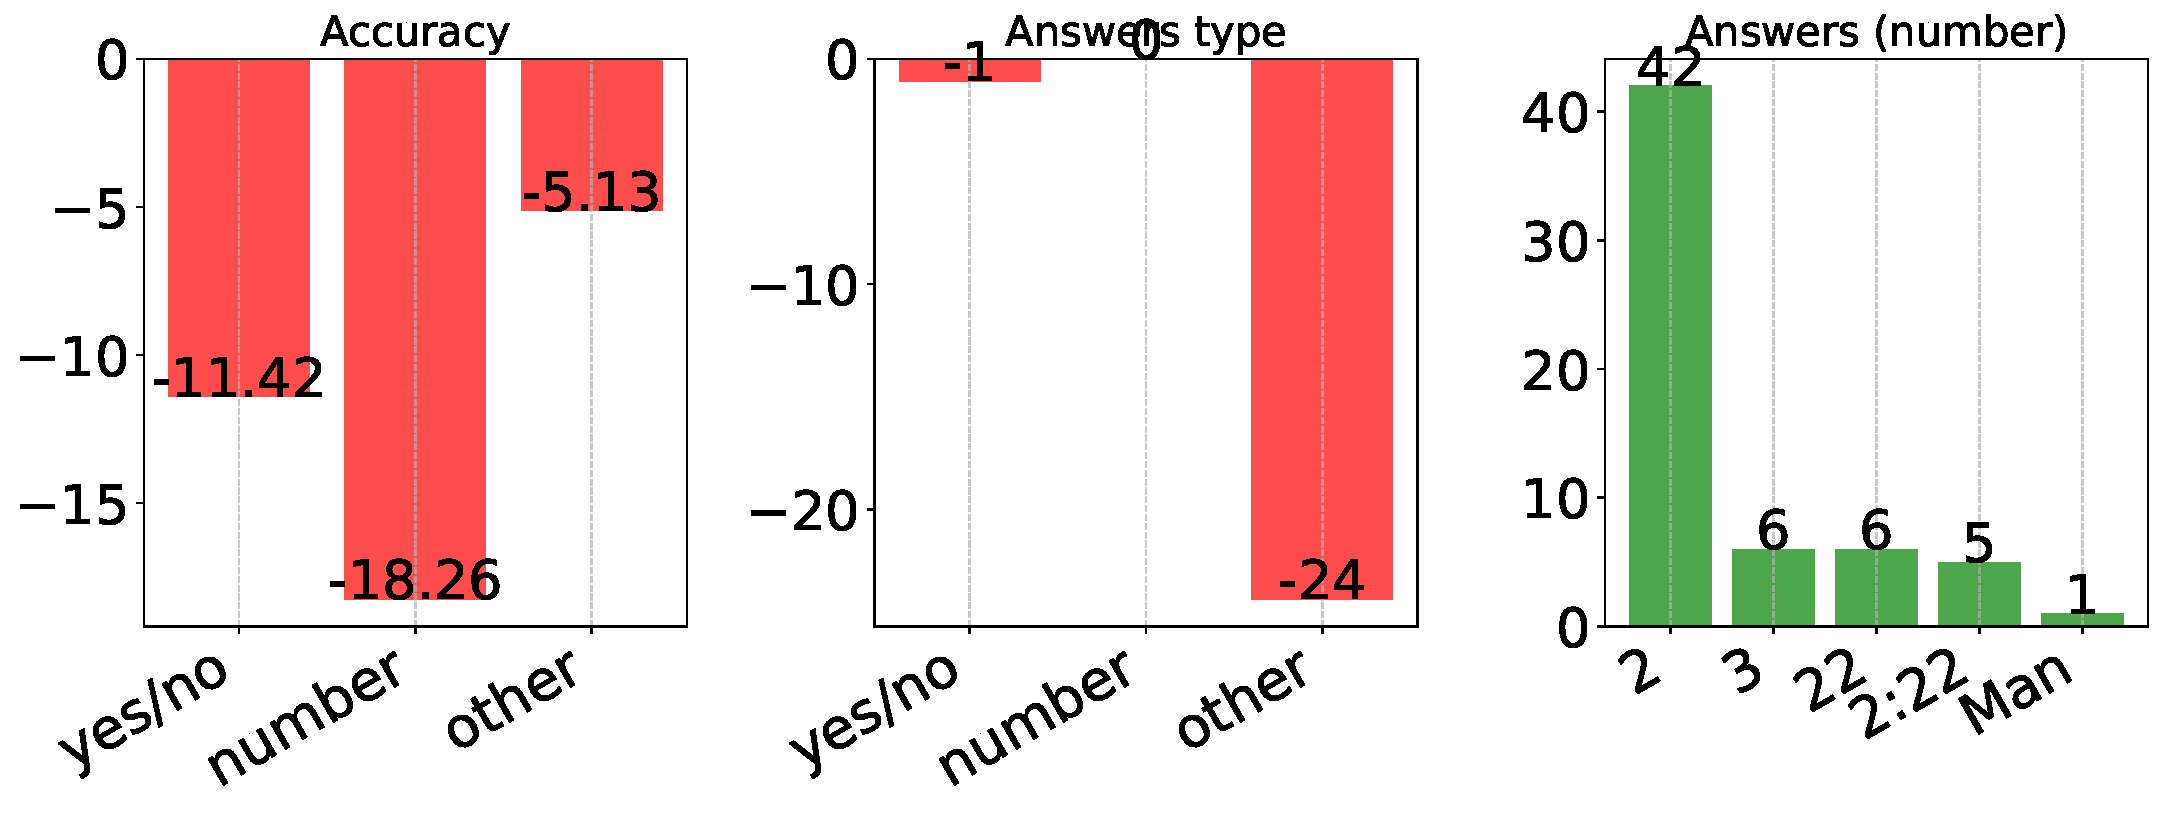
\includegraphics[width=1.0\textwidth]{Figures/model_steering/intra/steering_vector_vqav2_accuracy_llava_type_number_steering_vector_concept_3_to_5_only_target_answers.pdf}
        \end{minipage}%
        
        \begin{minipage}{\linewidth}
            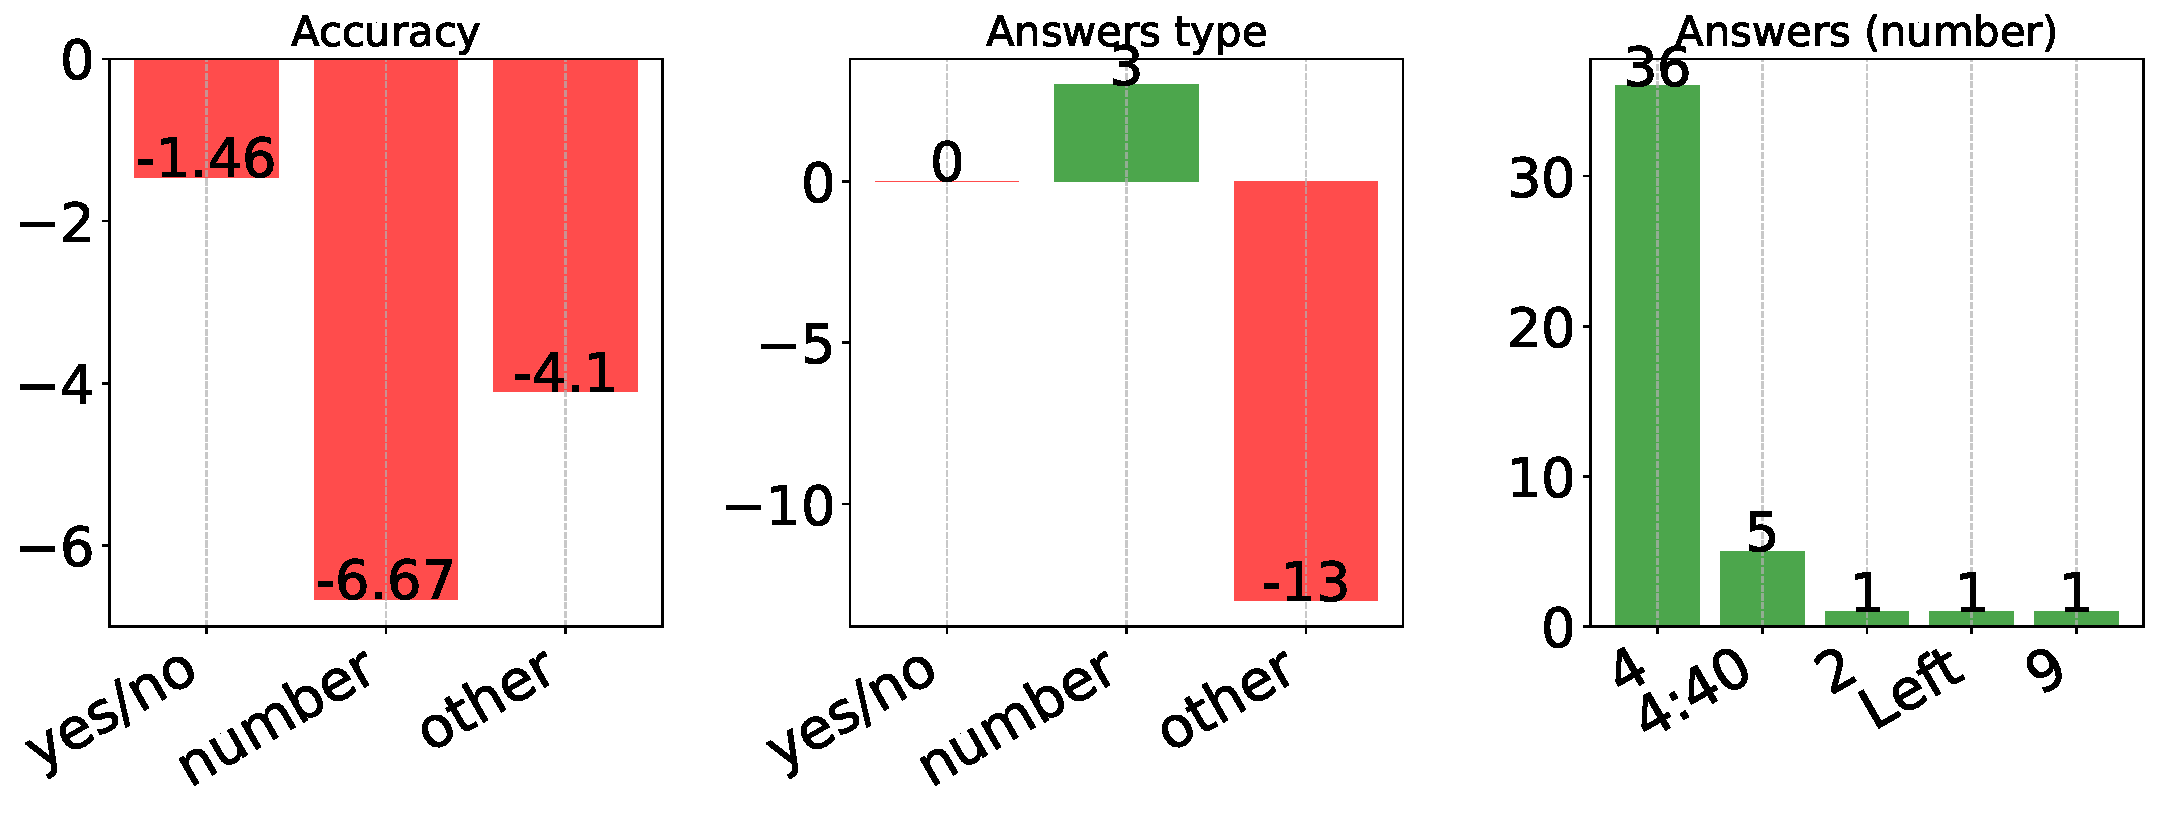
\includegraphics[width=1.0\textwidth]{Figures/model_steering/intra/steering_vector_vqav2_accuracy_llava_type_number_steering_vector_concept_0_to_2_only_target_answers.pdf}
        \end{minipage}%
        
    \end{minipage}%
\caption{\textbf{Discovering meaningful steering directions.} Each line corresponds to a finegrained steering direction to steer the model answer to (from top to bottom): "No" (yes/no), "Yes" (yes/no), "2" (number) and "4" (number). First line corresponds to the original model without steering. Some steering directions are targeted (\emph{e.g.}, "No") as there is slight change in both the accuracy on other types (\emph{e.g.}, number, other) and the number of answers type.}
\label{fig:app_model_steering_intra}
\end{figure}

\begin{figure}[!h]
    \centering
    \begin{minipage}{1\linewidth}
    \centering
        \begin{minipage}{\linewidth}
            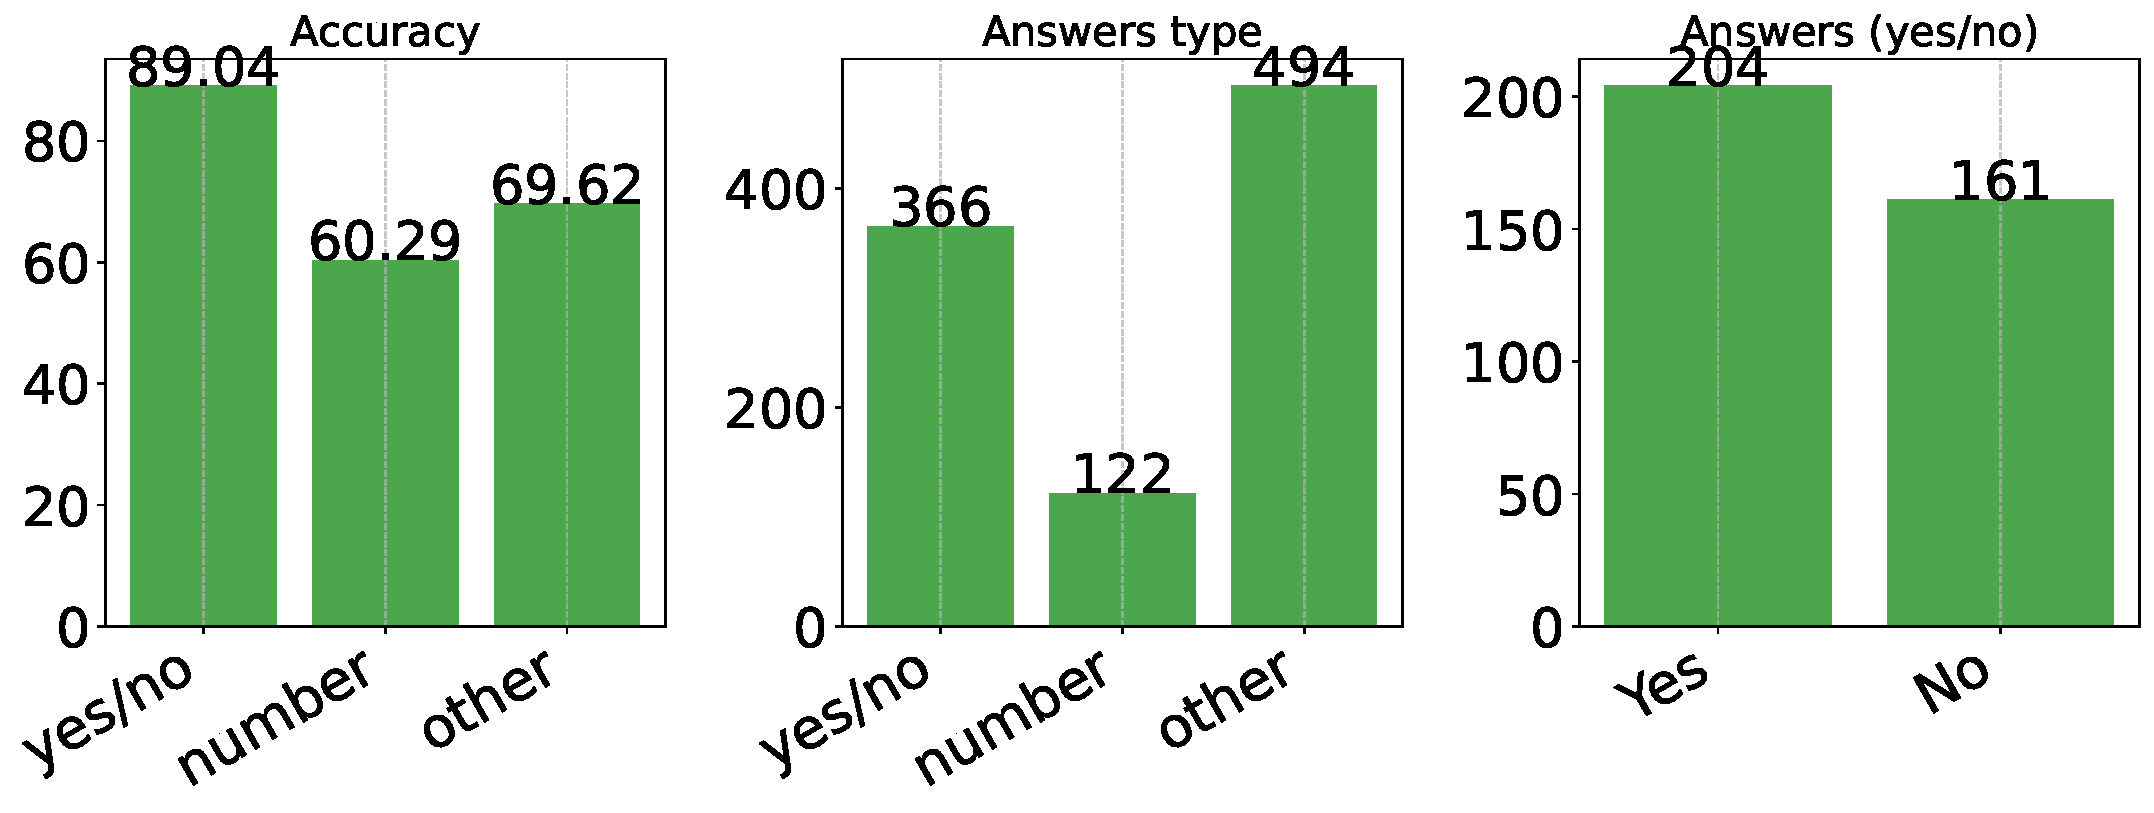
\includegraphics[width=1\textwidth]{Figures/model_steering/intra/steering_vector_vqav2_accuracy_llava_baseline_only_target_answers.pdf}
        \end{minipage}%
        
        \begin{minipage}{\linewidth}
            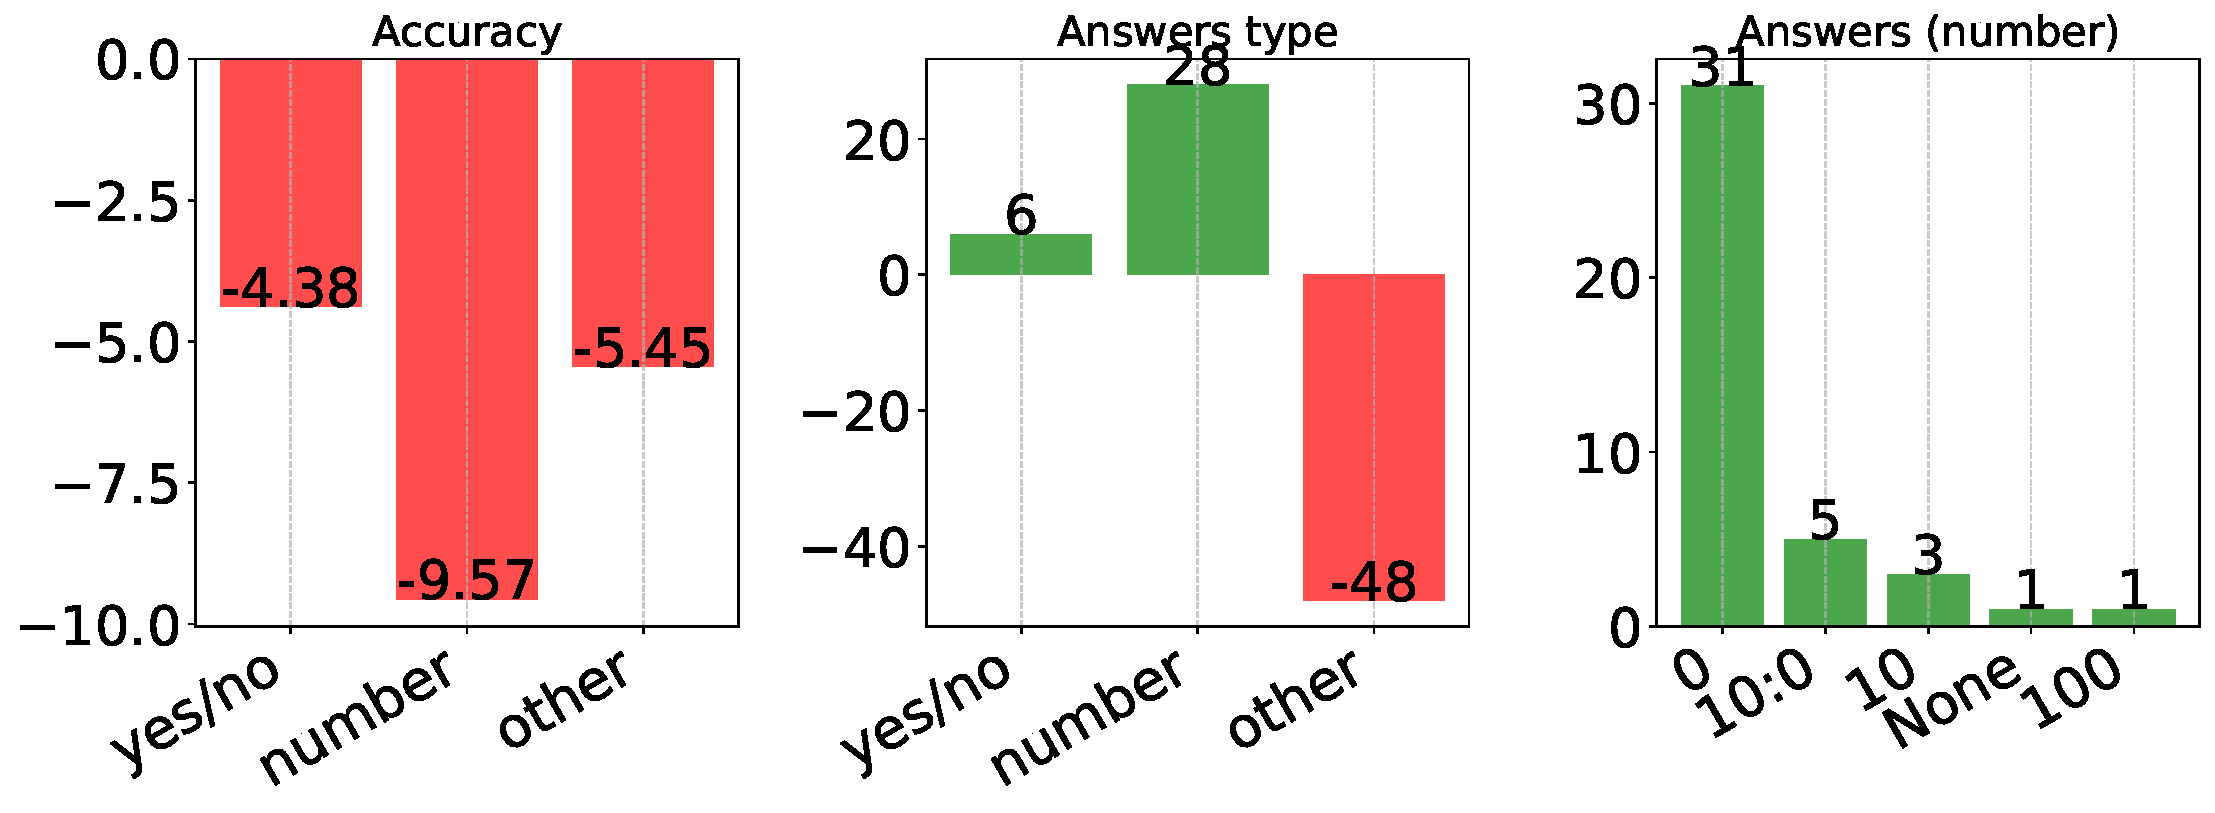
\includegraphics[width=1.0\textwidth]{Figures/model_steering/intra/steering_vector_vqav2_accuracy_llava_type_number_steering_vector_concept_7_to_8_only_target_answers.pdf}
        \end{minipage}%
        
        \begin{minipage}{\linewidth}
            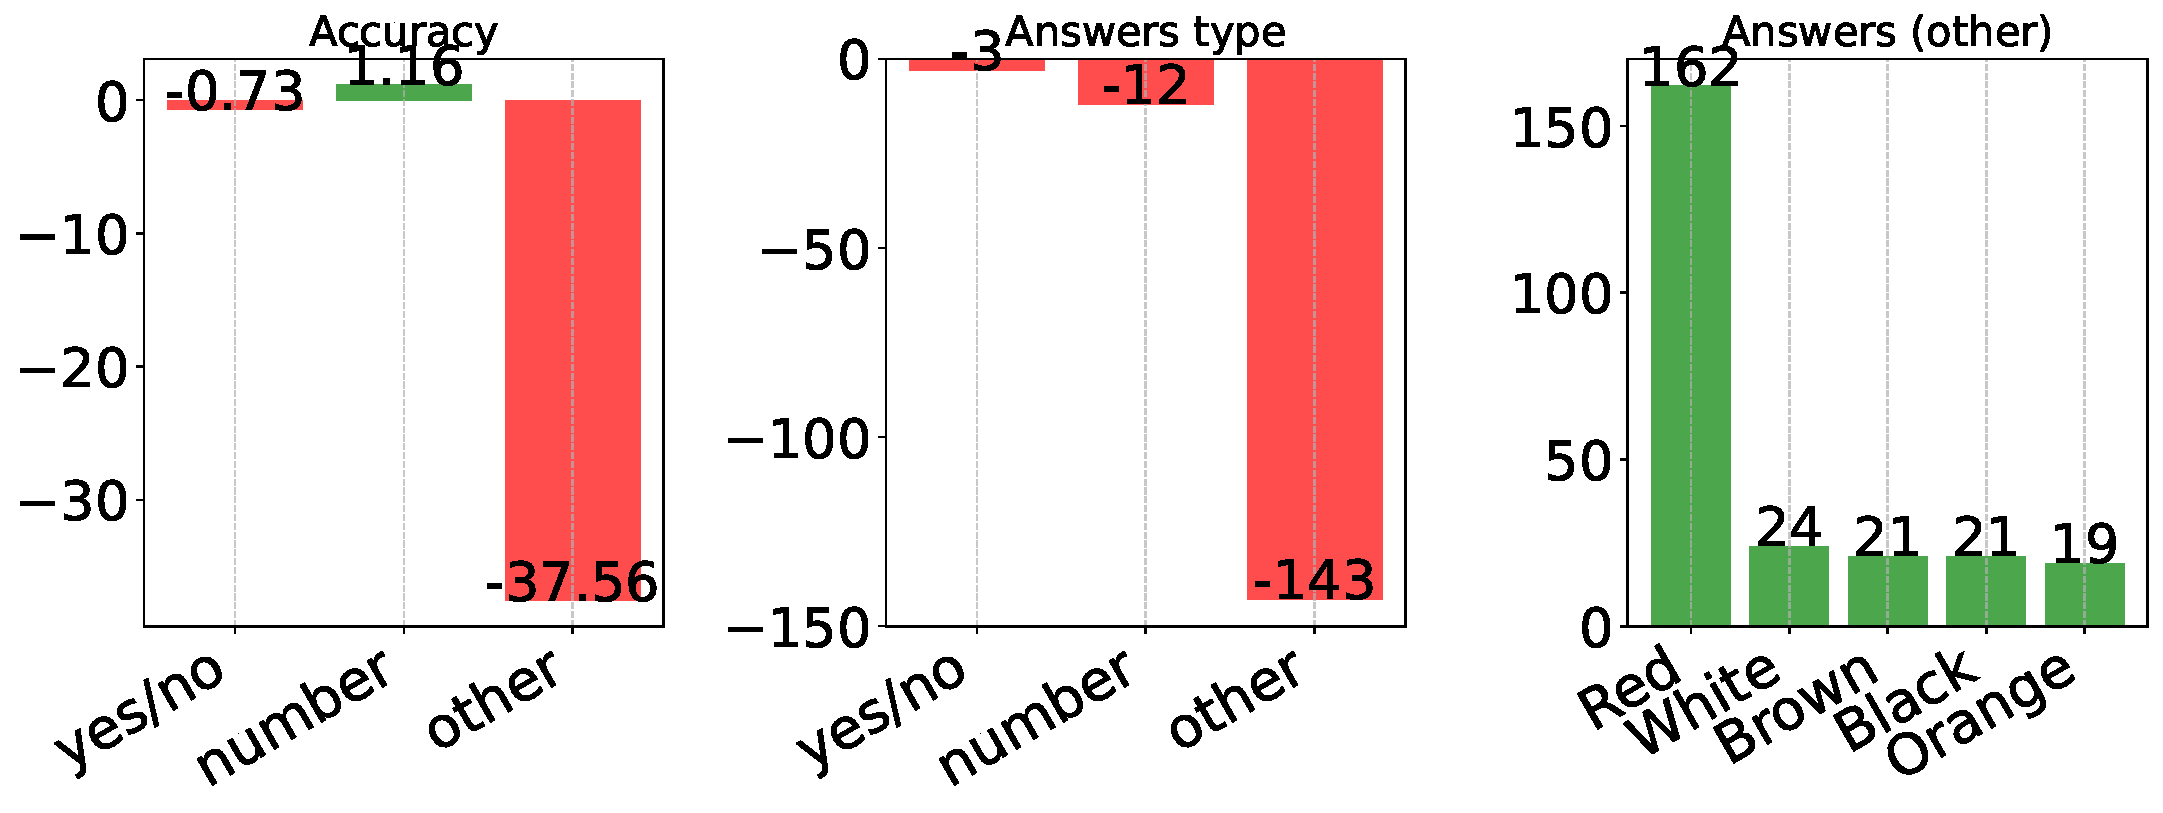
\includegraphics[width=1.0\textwidth]{Figures/model_steering/intra/steering_vector_vqav2_accuracy_llava_type_other_steering_vector_concept_4_to_9_only_target_answers.pdf}
        \end{minipage}%
        
        \begin{minipage}{\linewidth}
            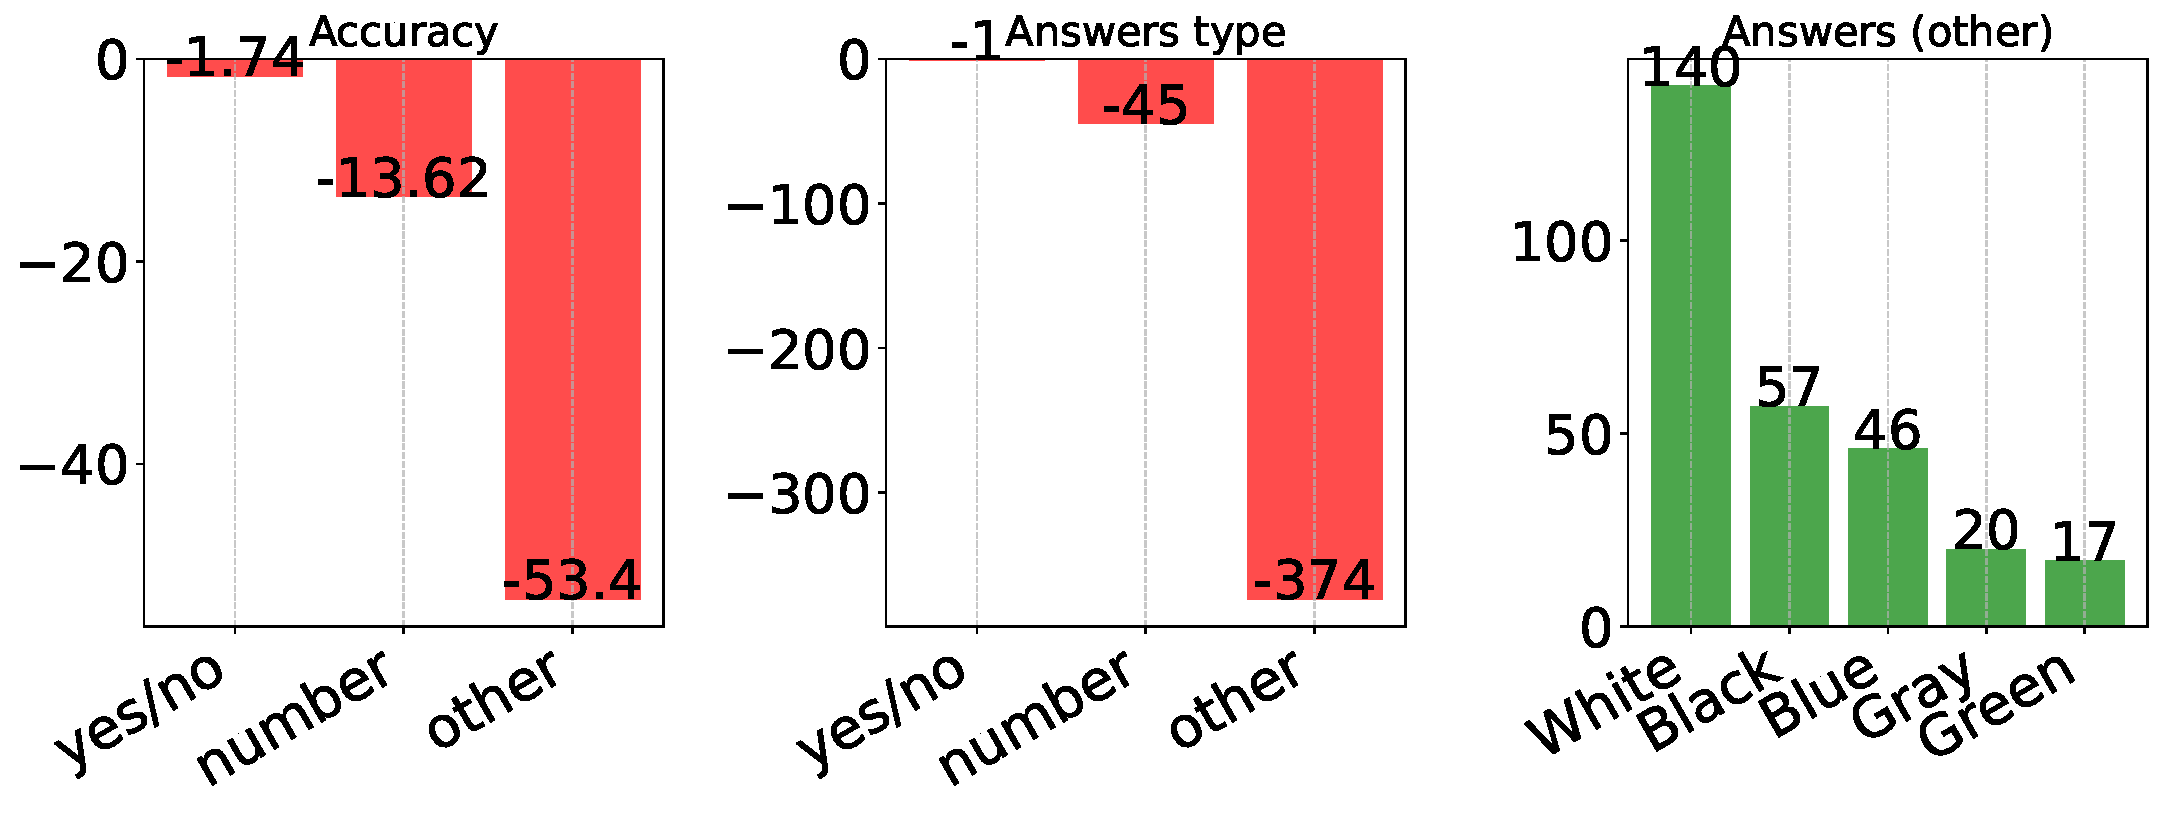
\includegraphics[width=1.0\textwidth]{Figures/model_steering/intra/steering_vector_vqav2_accuracy_llava_type_other_steering_vector_concept_0_to_2_only_target_answers.pdf}
        \end{minipage}%
        
        \begin{minipage}{\linewidth}
            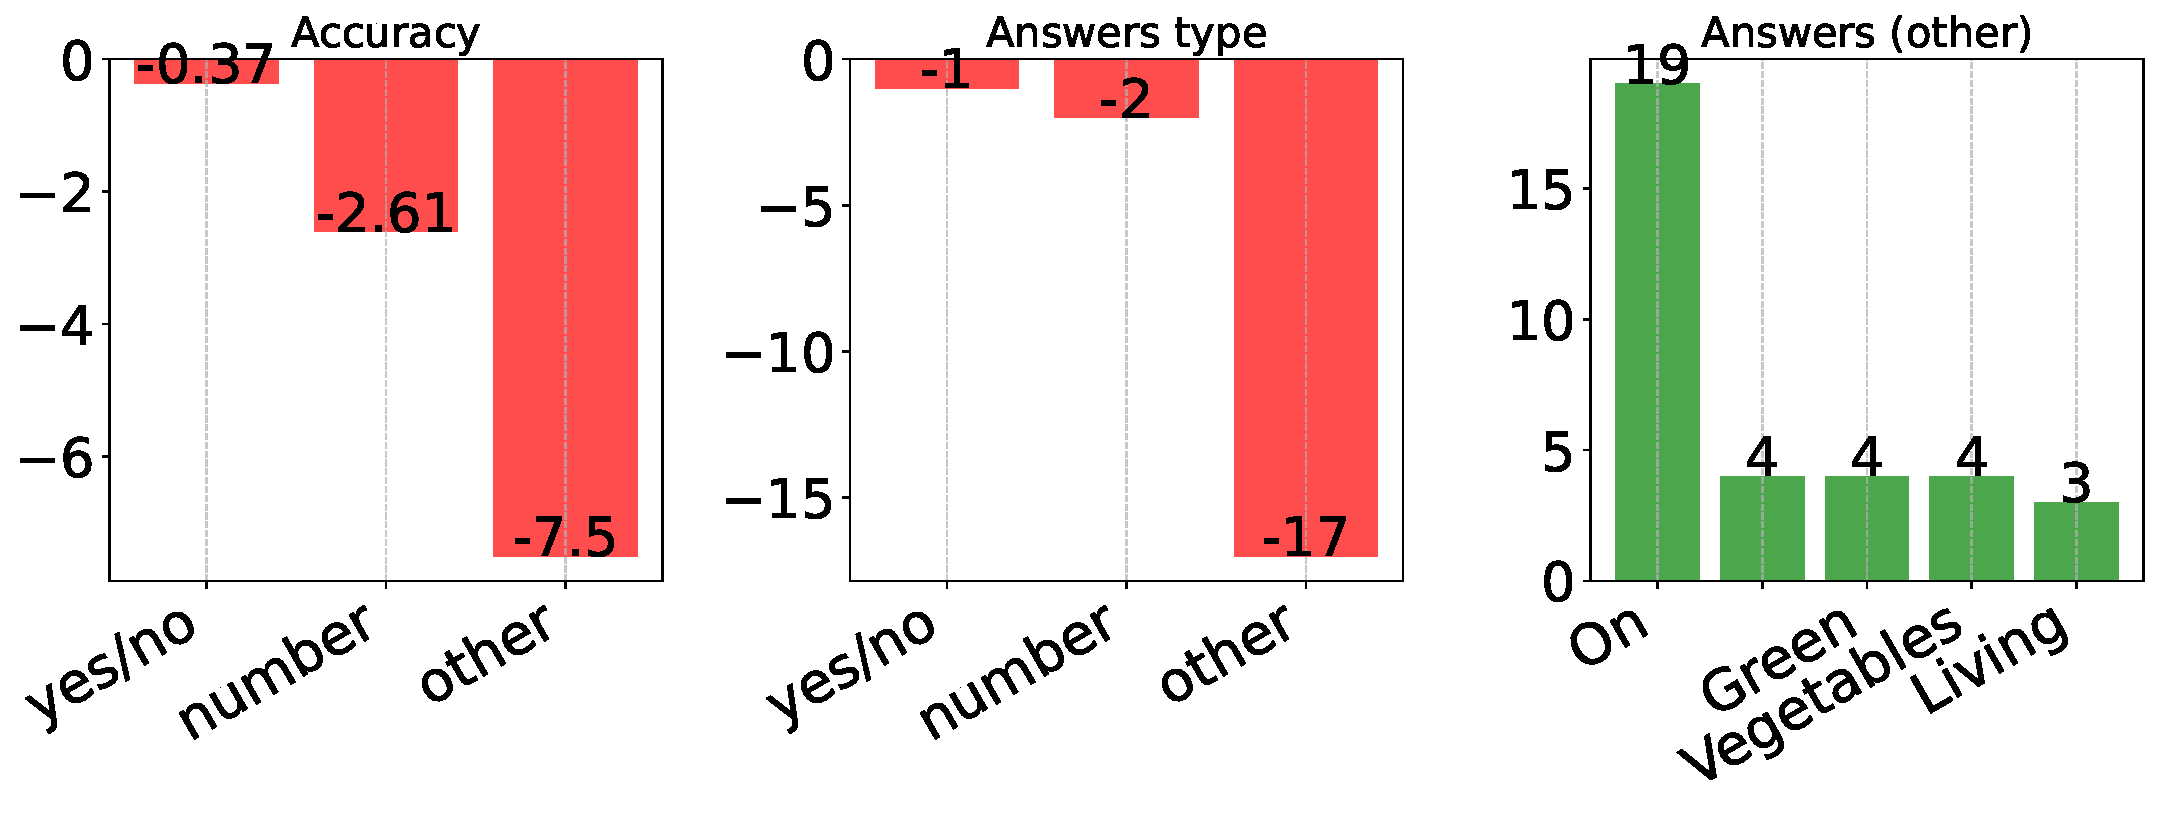
\includegraphics[width=1.0\textwidth]{Figures/model_steering/intra/steering_vector_vqav2_accuracy_llava_type_other_steering_vector_concept_1_to_9_only_target_answers.pdf}
        \end{minipage}%
    \end{minipage}%
\caption{\textbf{Discovering meaningful steering directions.} Each line corresponds to a finegrained steering direction to steer the model answer to: "0" (number), "Red" (other), "White" (other) and "On" (other). First line corresponds to the original model without steering.}
\label{fig:app_model_steering_intra2}
\end{figure}




\begin{figure}[!h]
    \centering
    \begin{minipage}{1\linewidth}
    \centering
        
        \begin{minipage}{\linewidth}
            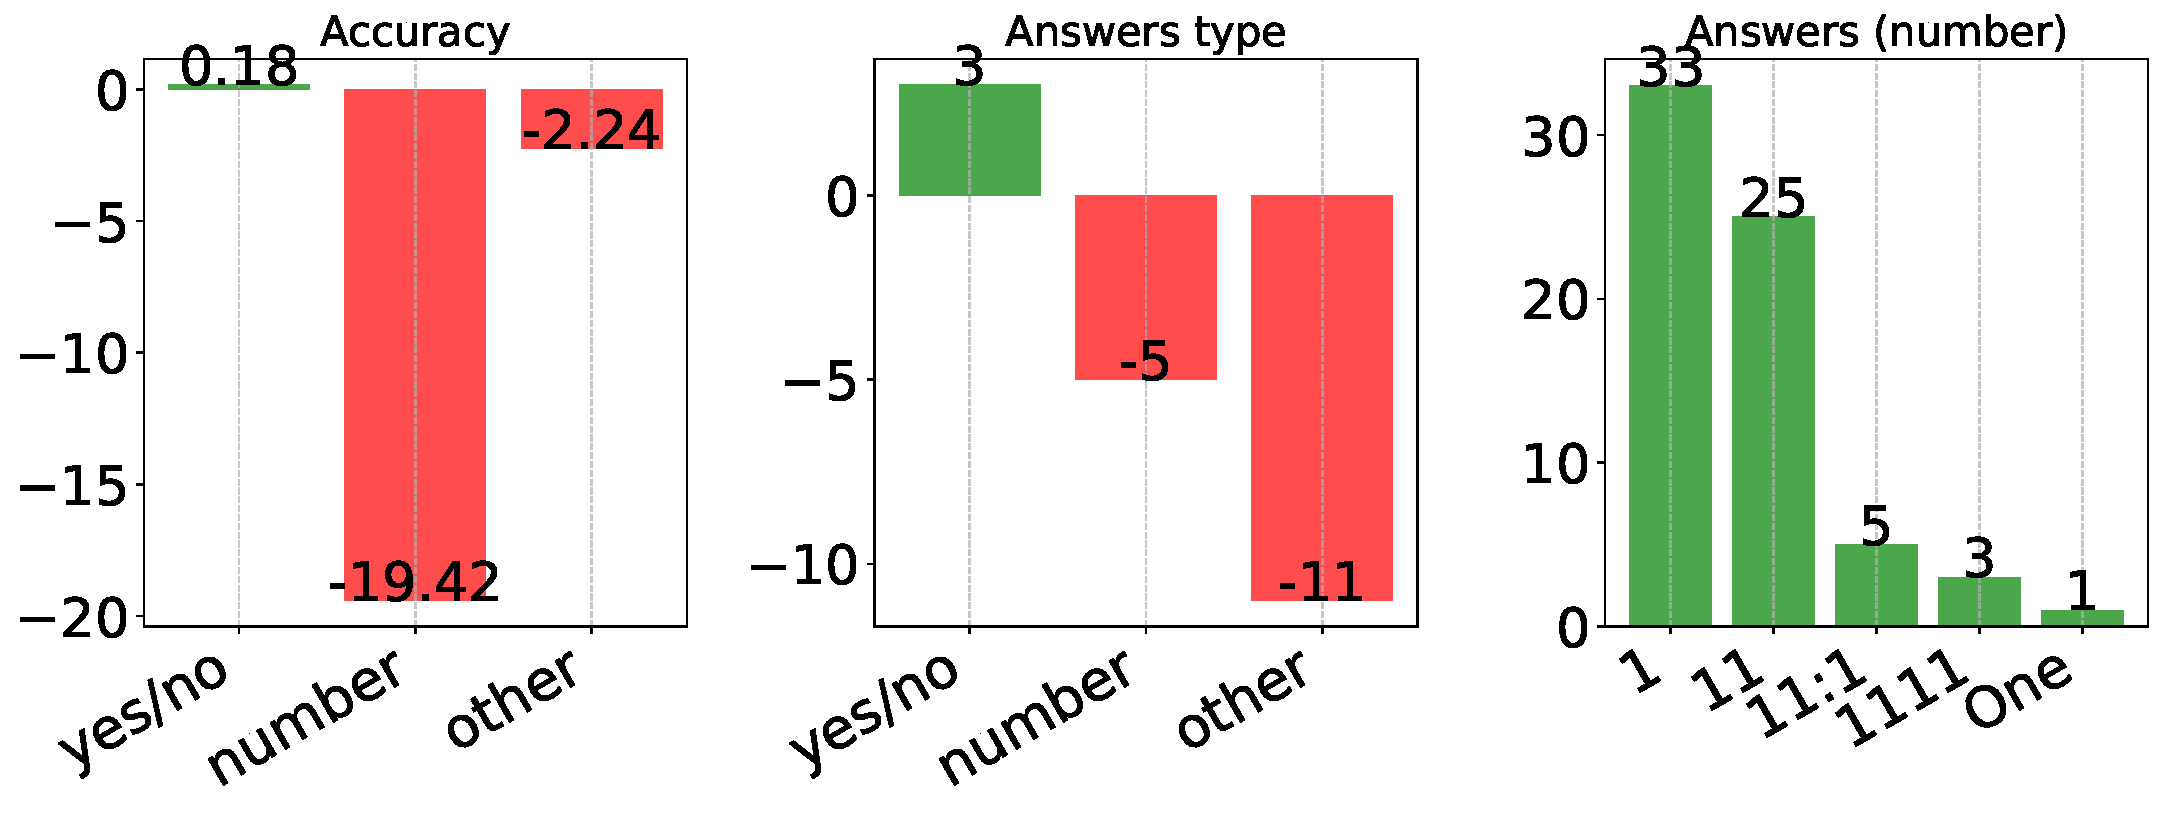
\includegraphics[width=1.0\textwidth]{Figures/model_steering/intra/steering_vector_vqav2_accuracy_llava_type_number_steering_vector_concept_2_to_3_only_target_answers_ntargetconcept_3.pdf}
        \end{minipage}%
        
        \begin{minipage}{\linewidth}
            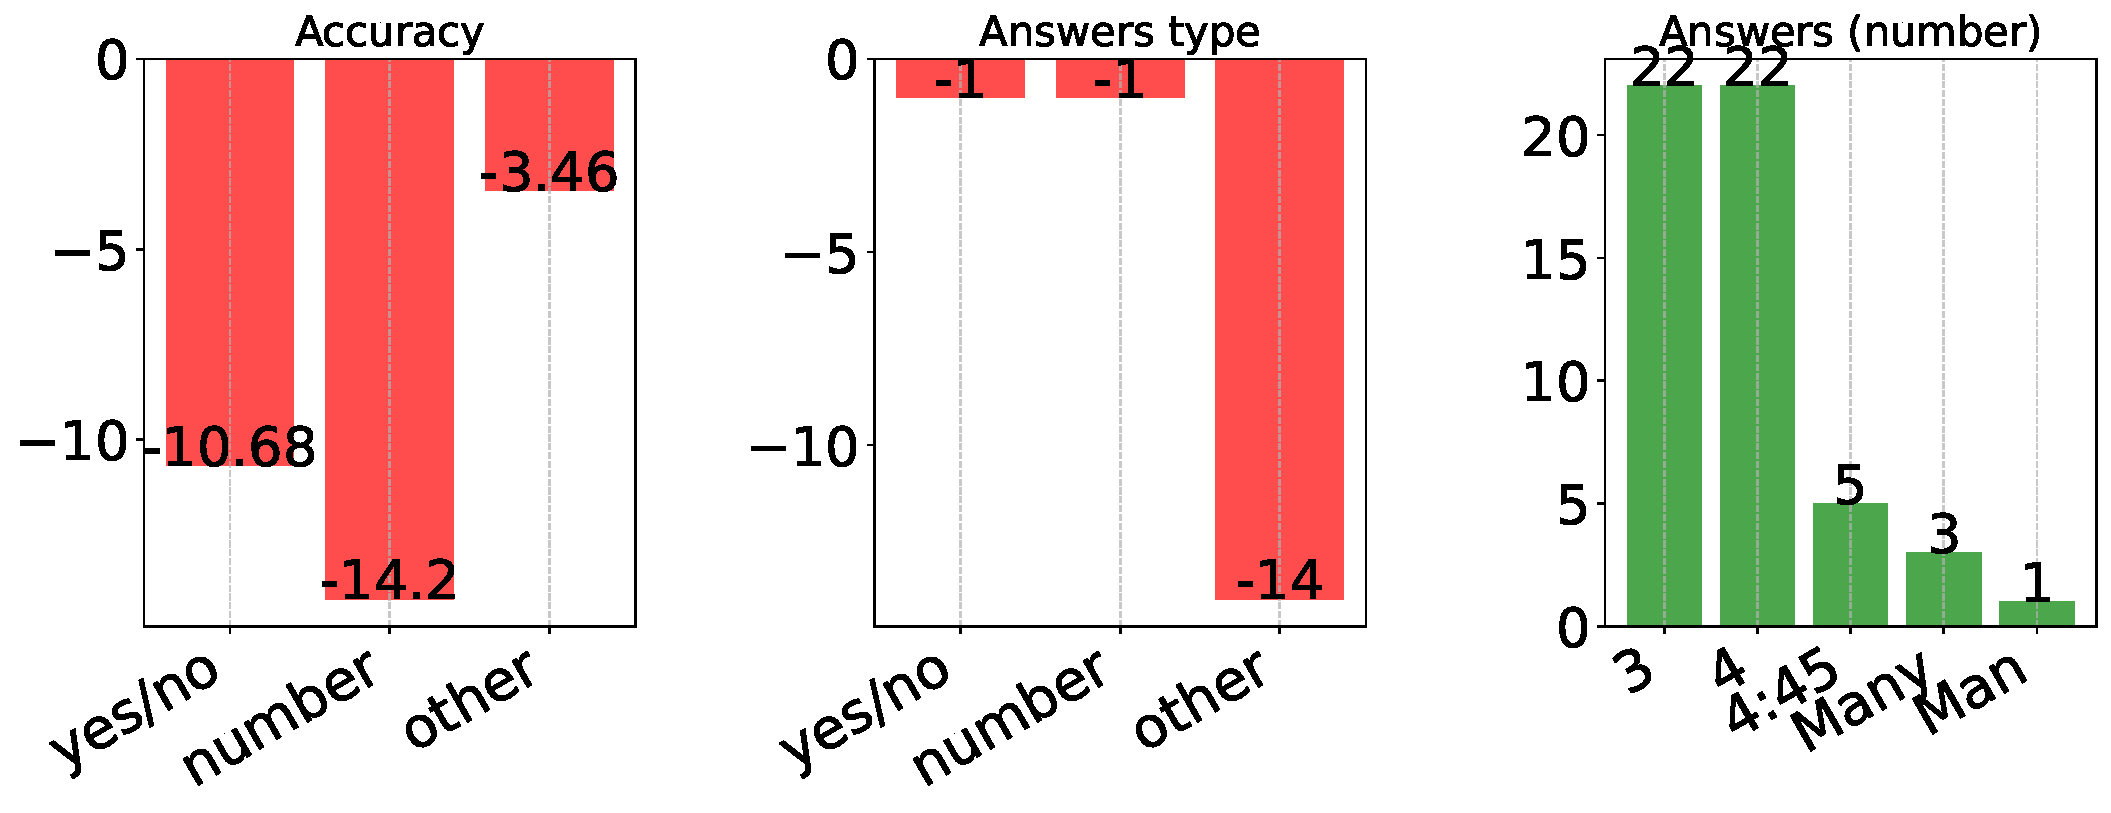
\includegraphics[width=1.0\textwidth]{Figures/model_steering/intra/steering_vector_vqav2_accuracy_llava_type_number_steering_vector_concept_1_to_5_only_target_answers_ntargetconcept_3.pdf}
        \end{minipage}%
        
        \begin{minipage}{\linewidth}
            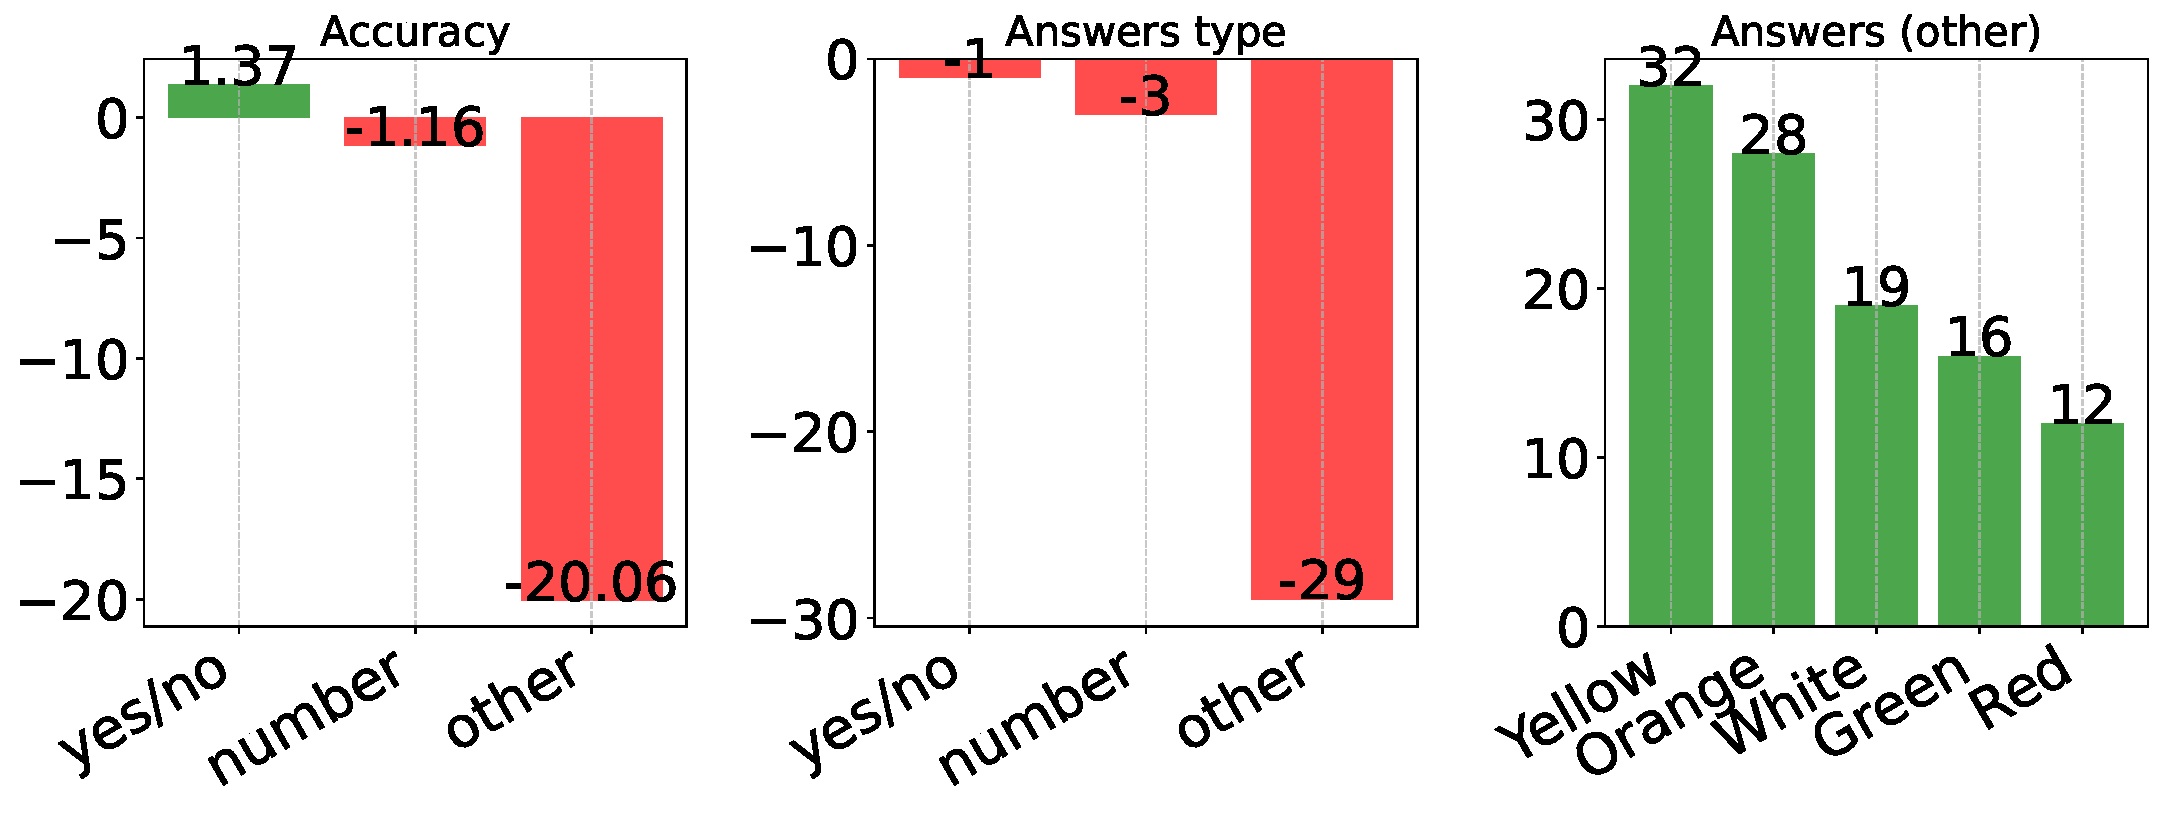
\includegraphics[width=1.0\textwidth]{Figures/model_steering/intra/steering_vector_vqav2_accuracy_llava_type_other_steering_vector_concept_6_to_9_only_target_answers_ntargetconcept_3.pdf}
        \end{minipage}%
        
        \begin{minipage}{\linewidth}
            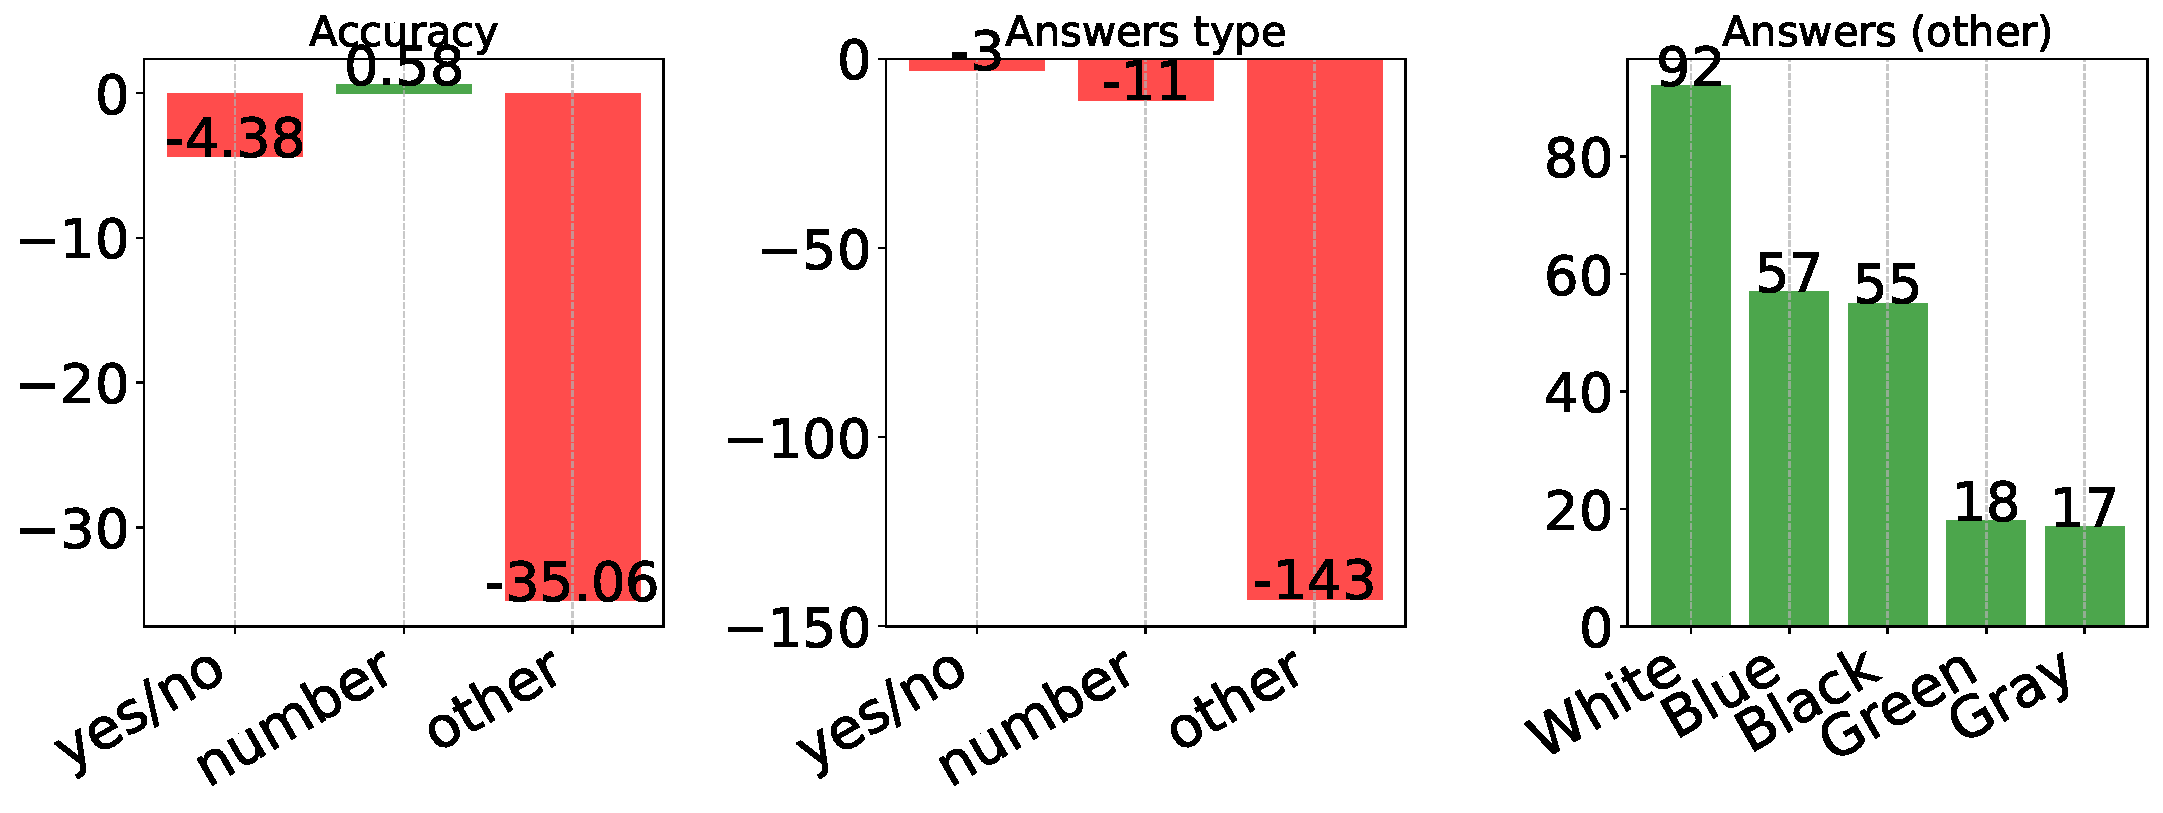
\includegraphics[width=1.0\textwidth]{Figures/model_steering/intra/steering_vector_vqav2_accuracy_llava_type_other_steering_vector_concept_0_to_7_only_target_answers_ntargetconcept_3.pdf}
        \end{minipage}%

        \begin{minipage}{\linewidth}
            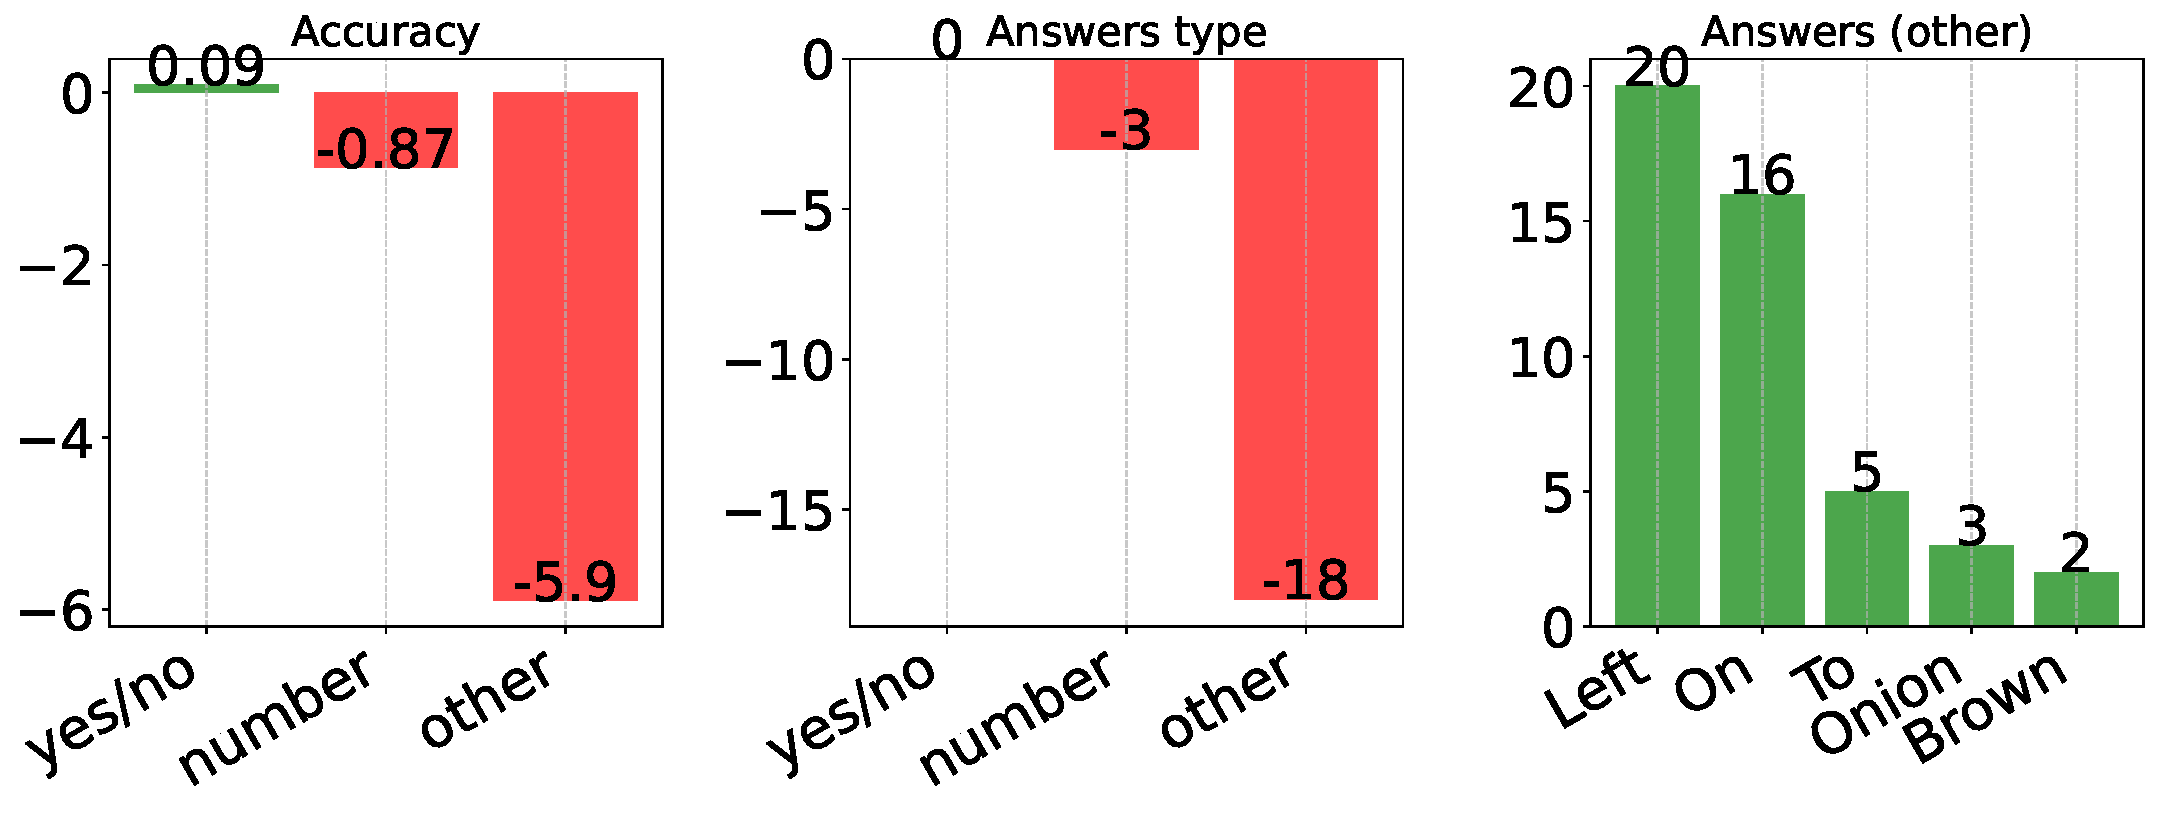
\includegraphics[width=1.0\textwidth]{Figures/model_steering/intra/steering_vector_vqav2_accuracy_llava_type_other_steering_vector_concept_7_to_8_only_target_answers_ntargetconcept_3.pdf}
        \end{minipage}%
        
    \end{minipage}%
\caption{\textbf{Discovering meaningful steering directions towards multiple concepts.} Each line corresponds to a finegrained steering direction to steer the model answer to (from top to bottom): "1" and "11" (number), "3" and "4" (number), "Yellow" and "Orange" (other), "White" and "Blue" (other) and "Left" and "On" (other).}
\label{fig:app_model_steering_intra_multiple}
\end{figure}

\subsection{Steering other MLLMs}
\label{sec:steering_other_models}


            





\begin{table*}[h]
    \centering
    \small
    \resizebox{0.8\linewidth}{!}{
        \begin{tabular}{lccccccccc}
        \toprule	 	
            \multirow{2}{*}{Model} 
            & \multirow{2}{*}{Steering} 
            & \multicolumn{3}{c}{Accuracy (\%)} 
            & \multicolumn{3}{c}{Answer Types} 
            & \multicolumn{2}{c}{Answers} \\
            \cmidrule(lr{8pt}){3-5}  
            \cmidrule(lr{8pt}){6-8} 
            \cmidrule(lr{8pt}){9-10}
            & 
            & Yes/No 
            & Number 
            & Other 
            & Yes/No 
            & Number 
            & Other 
            & Original 
            & Target \\
        \midrule
            \multirow{4}{*}{LLaVA-1.5} 
            & N/A 
            & 90.82 
            & 58.47 
            & 71.10 
            & 1861 
            & 687 
            & 2349 
            & 0 
            & 0 \\
            & Yes $\rightarrow$ No 
            & 69.03 
            & 56.82 
            & 68.99 
            & 1884 
            & 695 
            & 2294 
            & -828 
            & +828 \\
            & 1 $\rightarrow$ 3 
            & 90.71 
            & 54.52 
            & 71.12 
            & 1861 
            & 670 
            & 2350 
            & -215 
            & +144 \\
            & White $\rightarrow$ Black 
            & 90.40 
            & 58.42 
            & 58.36 
            & 1861 
            & 671 
            & 2312 
            & -98 
            & +441 \\
        \midrule
            \multirow{4}{*}{Qwen2-VL-Instruct} 
            & N/A 
            & 95.20 
            & 77.31 
            & 74.67 
            & 1861 
            & 676 
            & 2343 
            & 0 
            & 0 \\
            & Yes $\rightarrow$ No 
            & 64.96 
            & 58.37 
            & 40.83 
            & 3034 
            & 608 
            & 1176 
            & -900 
            & +901 \\
            & 1 $\rightarrow$ 3 
            & 95.33 
            & 41.68 
            & 74.15 
            & 1859 
            & 671 
            & 2346 
            & -187 
            & +291 \\
            & White $\rightarrow$ Black 
            & 95.28 
            & 76.41 
            & 68.27 
            & 1863 
            & 683 
            & 2334 
            & -92 
            & +176 \\
        \midrule
            \multirow{4}{*}{Idefics2} 
            & N/A 
            & 93.77 
            & 62.57 
            & 73.77 
            & 1851 
            & 657 
            & 2342 
            & 0 
            & 0 \\
            & Yes $\rightarrow$ No 
            & 64.96 
            & 61.47 
            & 62.24 
            & 2362 
            & 654 
            & 1807 
            & -906 
            & +907 \\
            & 1 $\rightarrow$ 3 
            & 94.11 
            & 39.23 
            & 72.94 
            & 1850 
            & 668 
            & 2323 
            & -104 
            & +118 \\
            & White $\rightarrow$ Black 
            & 93.77 
            & 62.82 
            & 64.33 
            & 1855 
            & 659 
            & 2322 
            & -95 
            & +396 \\
        \bottomrule
        \end{tabular}
    }
    \caption{\textbf{Steering MLLMs answers.} Steering answers from "Yes" (yes/no), "1" (number), "White" (other) to "No", "3", "Black" respectively. The number of original/target answer counts decrease/increase significantly, while the accuracy on other answer types changes slightly, and the number of answer type counts remains almost constant. Steering at layer: last (LLaVA-1.5), 23 (Qwen2-VL), 25 (Idefics2).}
    \label{tab:model_steering_answers_other_models}
\end{table*}



\subsection{Discovering meaningful steering directions.}
\label{sec:app_model_steering_discover_concepts}

\paragraph{Steering vectors selection metric.} Not all computed vectors are necessarily meaningful steering vectors. We identify those that are meaningful, as those with the strongest impact on guiding the model towards generating specific answers or concepts. The selection process follows these steps:

\begin{itemize} 
    \item For each steering vector in a set, apply it to steer the model's behavior. 
    \item Measure the change in the answers number of occurrence between the steered model and the original model, producing the count of relative occurrences for each answer. 
    \item For each vector, keep the top N answers with the highest relative occurrence counts. 
    \item Use k-means (k=2) to cluster the top N answers. 
    \item Assign each answer to one of the two clusters. The primary answers are those belonging to the cluster with the highest total occurrences. These answers are considered the target answers for the steering vector.
    \item Calculate the difference in relative occurrence between primary answers and those in the secondary cluster. 
    \item Select the steering directions that exhibit the highest differences in relative occurrence between clusters. This is considered our selection score.
\end{itemize}
    
We use clustering to accommodate the possibility of steering multiple concepts at a time.


\paragraph{Steering directions towards a single concept.} Following our selection process discussed previously, we illustrate some of the steering vectors that have the highest selection score. We decompose the clusters from 3 answers type: colors, numbers and other. \Cref{fig:app_model_steering_intra} and \Cref{fig:app_model_steering_intra2} shows that the vectors corresponds to steering the model towards very specific answer, such as No, Red and 4.


\paragraph{Steering directions towards multiple concepts.} We can also find vectors that steer the model towards more than one answer, this is because some concepts might encompass different answers. \Cref{fig:app_model_steering_intra_multiple} shows that some steering vectors corresponds to "3" and "4" or "Yellow" and "Orange".



\begin{figure*}[!h]
    \centering
    \begin{minipage}{0.9\linewidth}
    \centering
        \begin{minipage}{0.24\linewidth}
            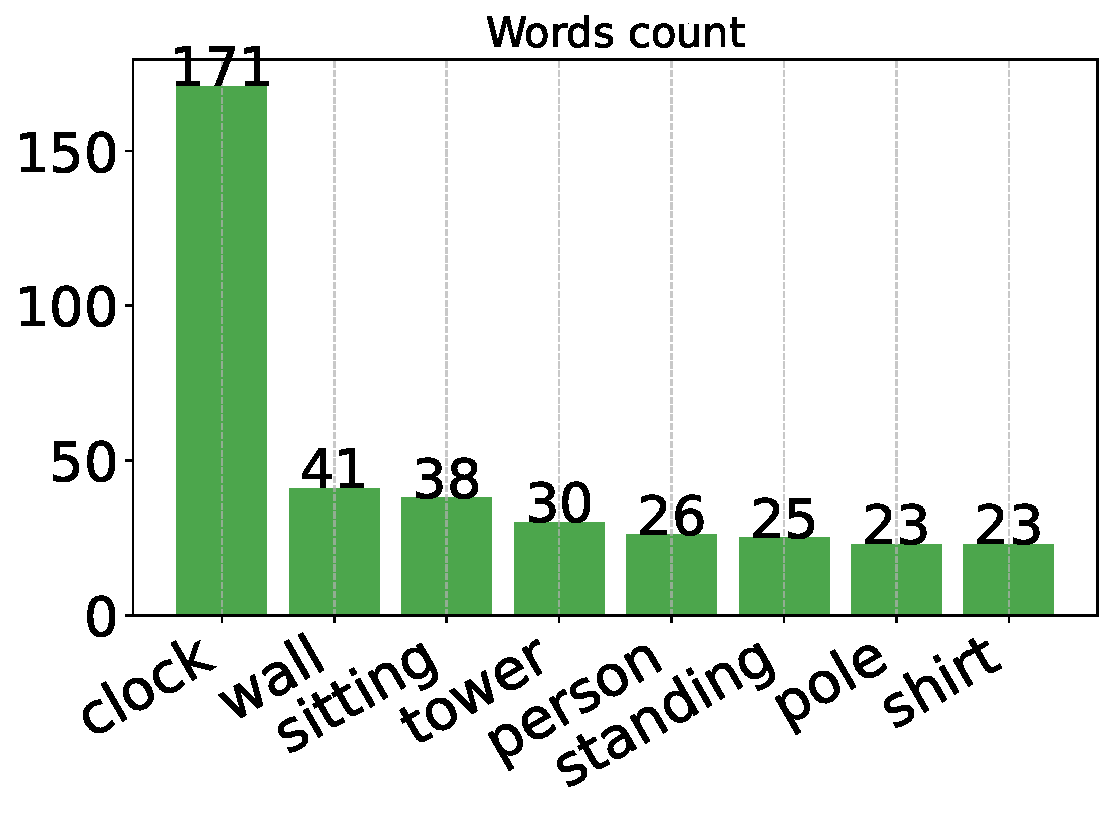
\includegraphics[width=1.0\textwidth]{Figures/model_steering/intra/coco/captioning_metrics_intra_llava_19_places_onlytoi_steering_vector_concept_0_to_1_d_1000_ntcon_1.pdf}
        \end{minipage}%
        \begin{minipage}{0.24\linewidth}
            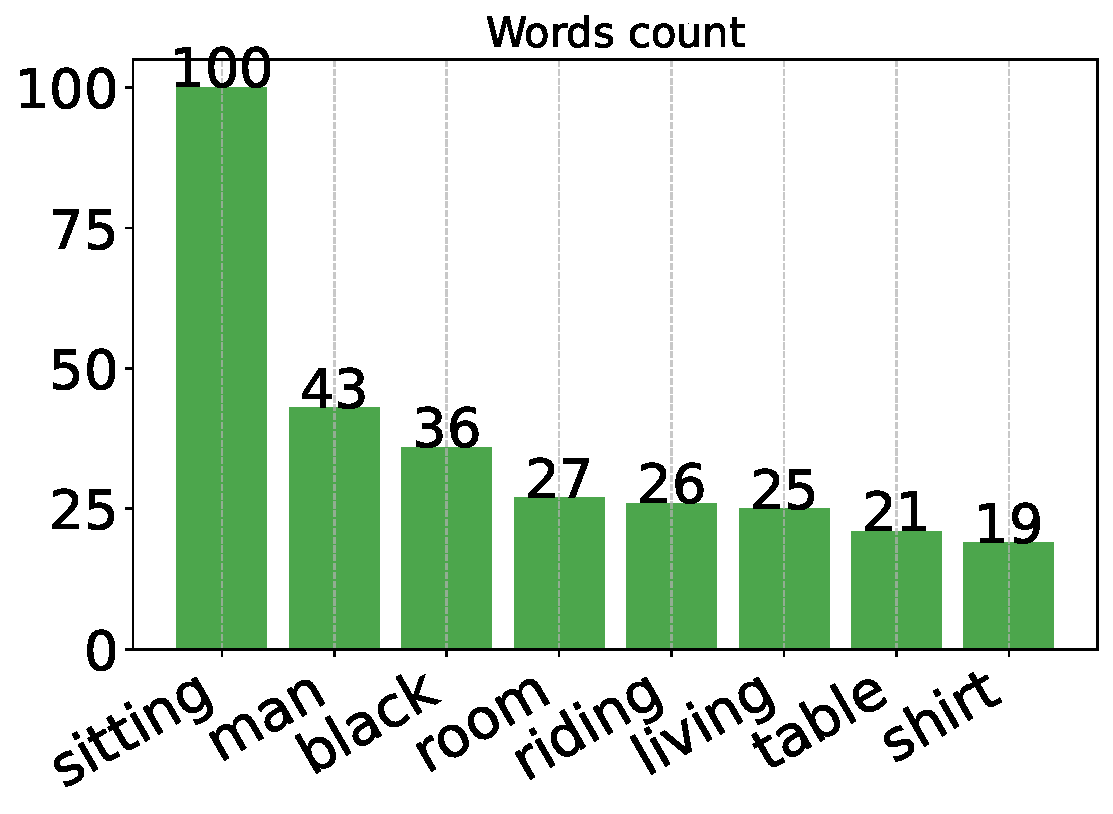
\includegraphics[width=1.0\textwidth]{Figures/model_steering/intra/coco/captioning_metrics_intra_llava_19_places_onlytoi_steering_vector_concept_0_to_2_d_1000_ntcon_1.pdf}
        \end{minipage}%
        \begin{minipage}{0.24\linewidth}
            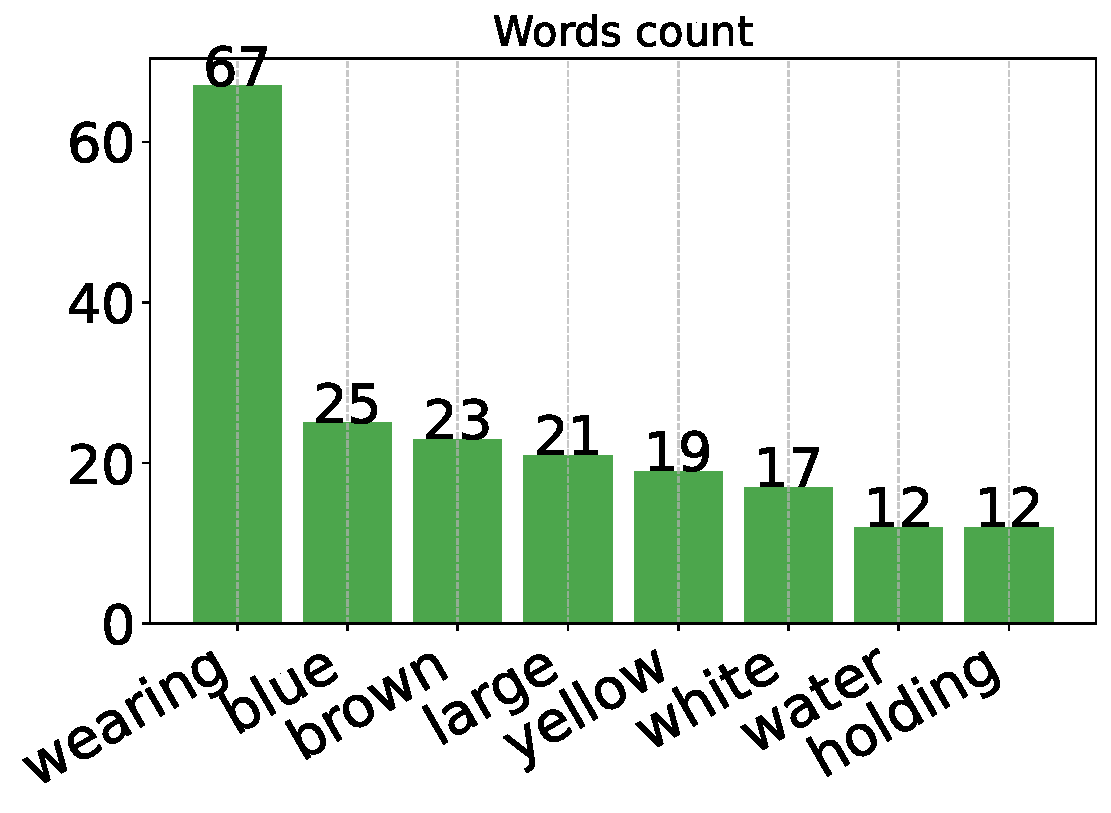
\includegraphics[width=1.0\textwidth]{Figures/model_steering/intra/coco/captioning_metrics_intra_llava_19_places_onlytoi_steering_vector_concept_0_to_3_d_1000_ntcon_1.pdf}
        \end{minipage}%
        \begin{minipage}{0.24\linewidth}
            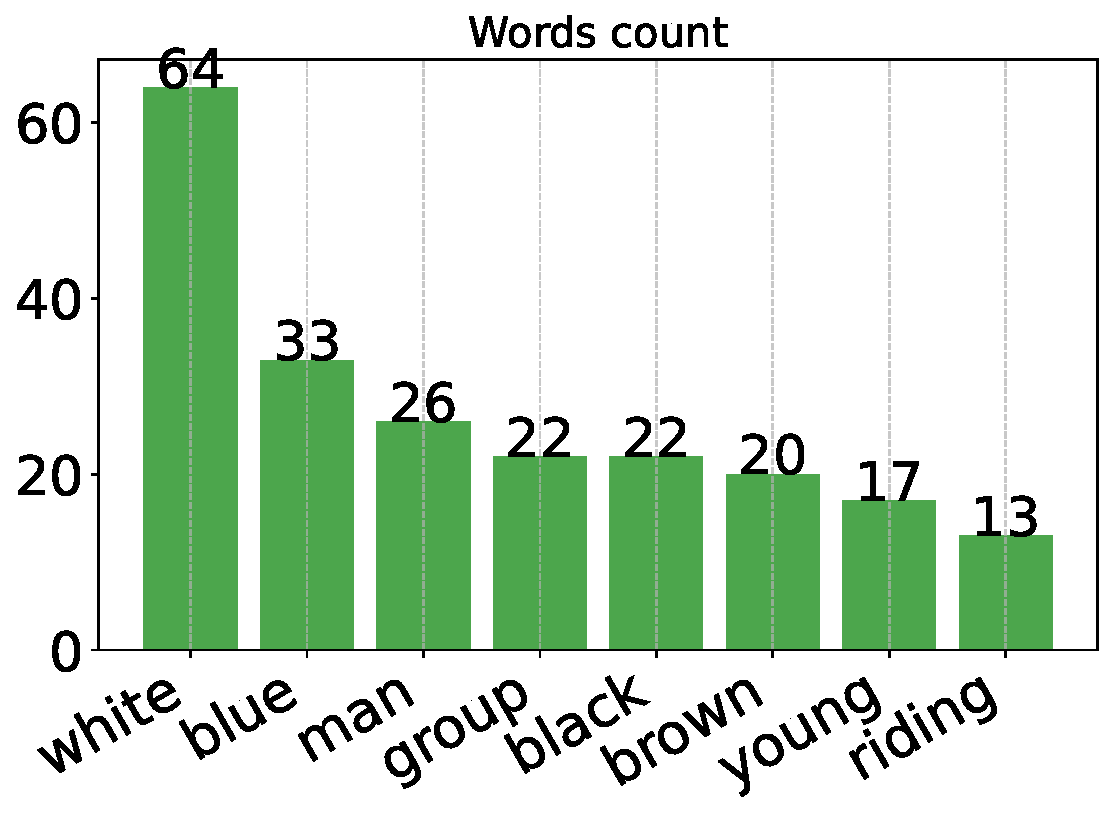
\includegraphics[width=1.0\textwidth]{Figures/model_steering/intra/coco/captioning_metrics_intra_llava_19_places_onlytoi_steering_vector_concept_0_to_4_d_1000_ntcon_1.pdf}
        \end{minipage}%
        
        \begin{minipage}{0.24\linewidth}
            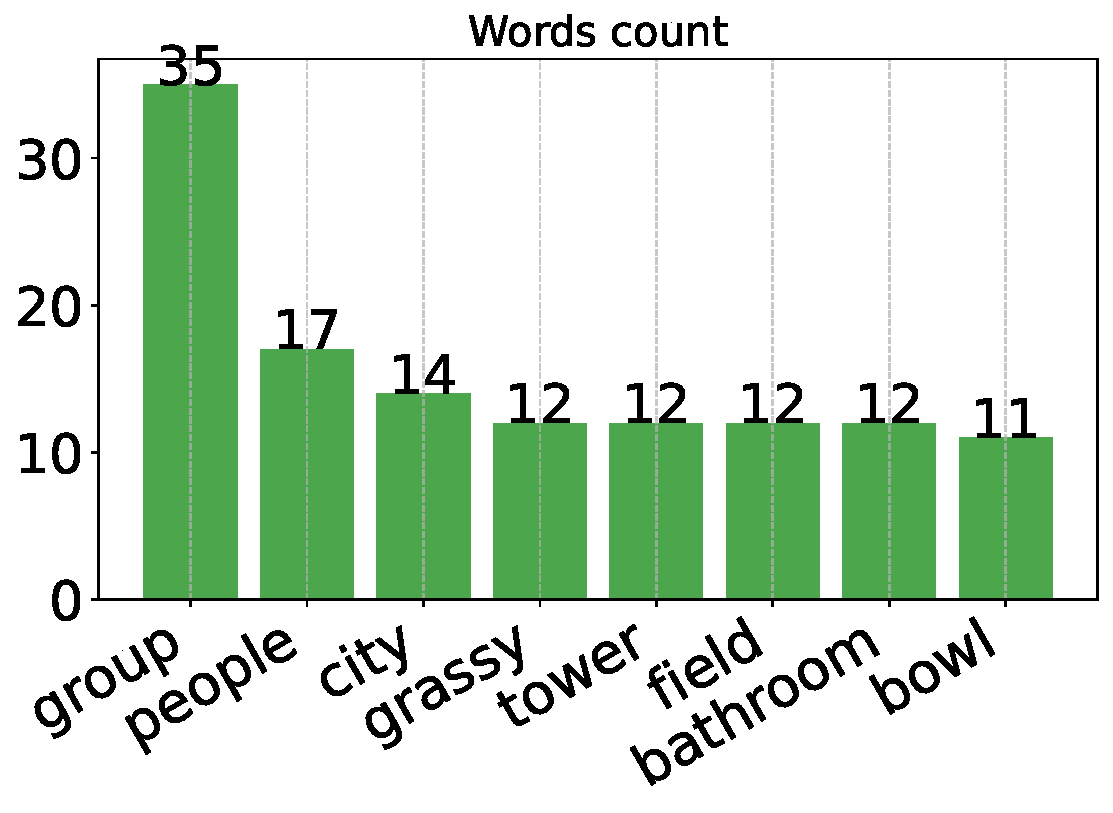
\includegraphics[width=1.0\textwidth]{Figures/model_steering/intra/coco/captioning_metrics_intra_llava_19_places_onlytoi_steering_vector_concept_0_to_5_d_1000_ntcon_1.pdf}
        \end{minipage}%
        \begin{minipage}{0.24\linewidth}
            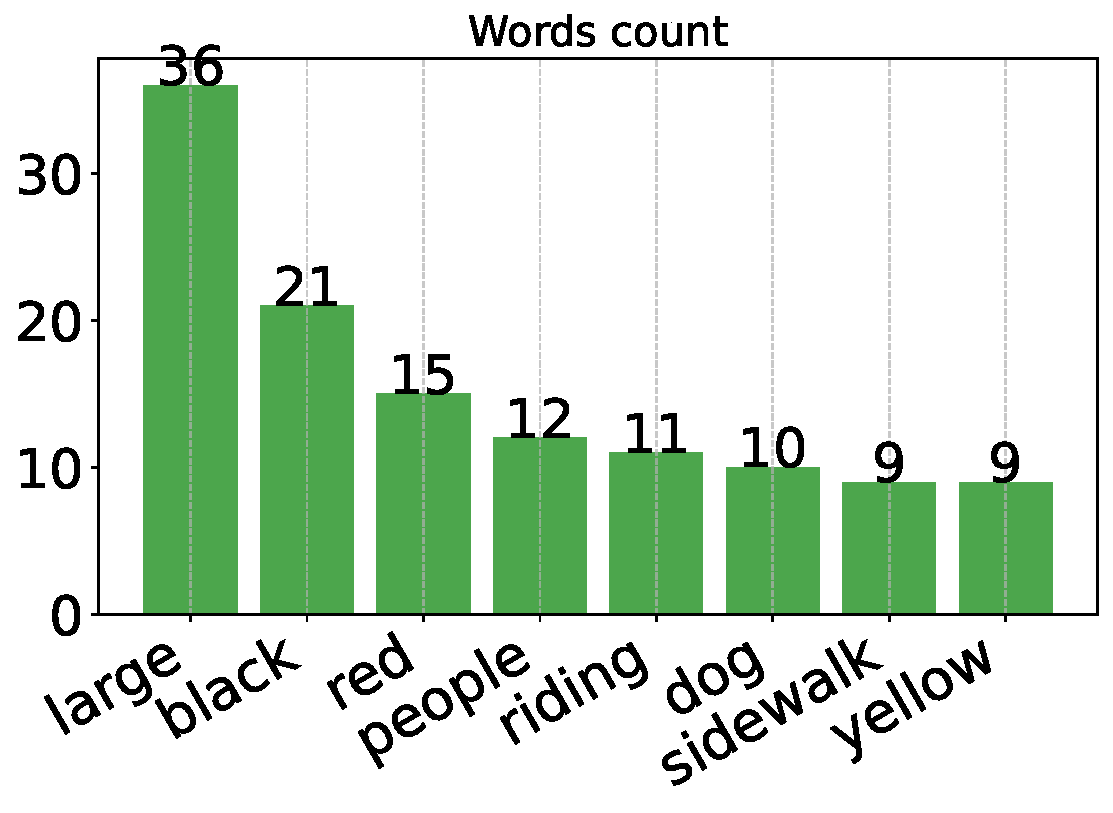
\includegraphics[width=1.0\textwidth]{Figures/model_steering/intra/coco/captioning_metrics_intra_llava_19_places_onlytoi_steering_vector_concept_0_to_6_d_1000_ntcon_1.pdf}
        \end{minipage}%
        \begin{minipage}{0.24\linewidth}
            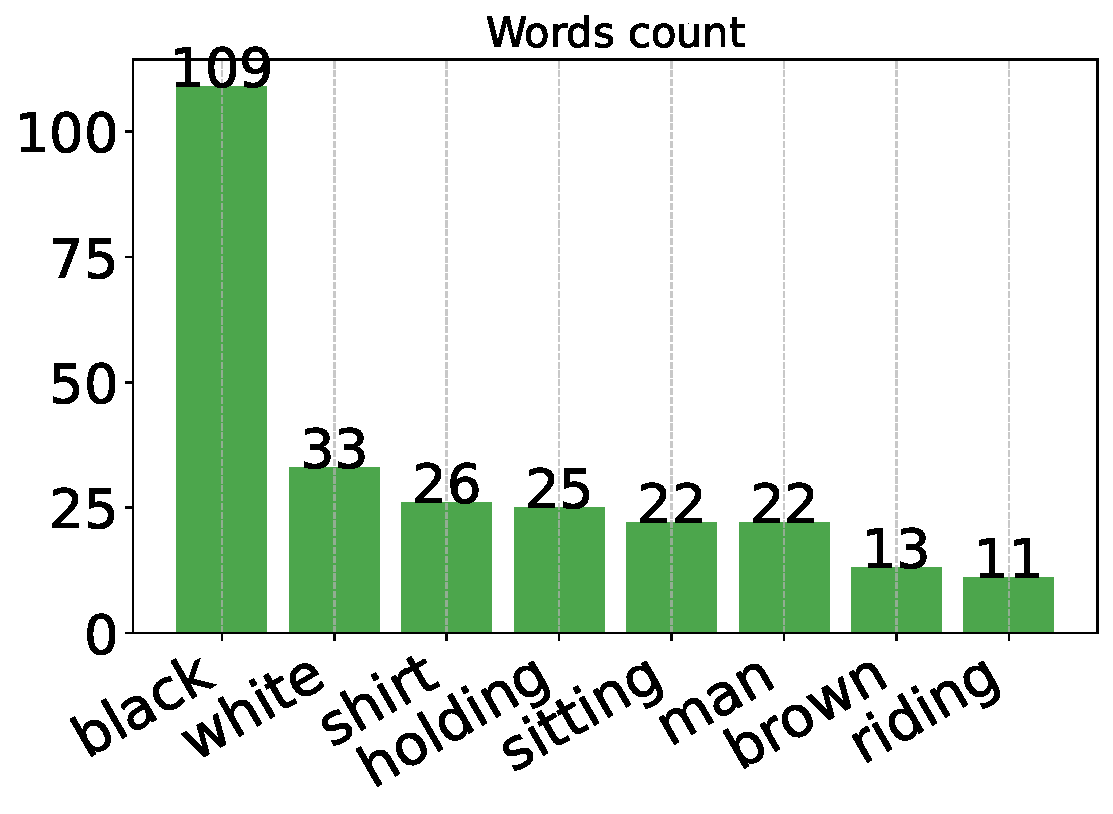
\includegraphics[width=1.0\textwidth]{Figures/model_steering/intra/coco/captioning_metrics_intra_llava_19_colors_onlytoi_steering_vector_concept_0_to_2_d_1000_ntcon_1.pdf}
        \end{minipage}%
        \begin{minipage}{0.24\linewidth}
            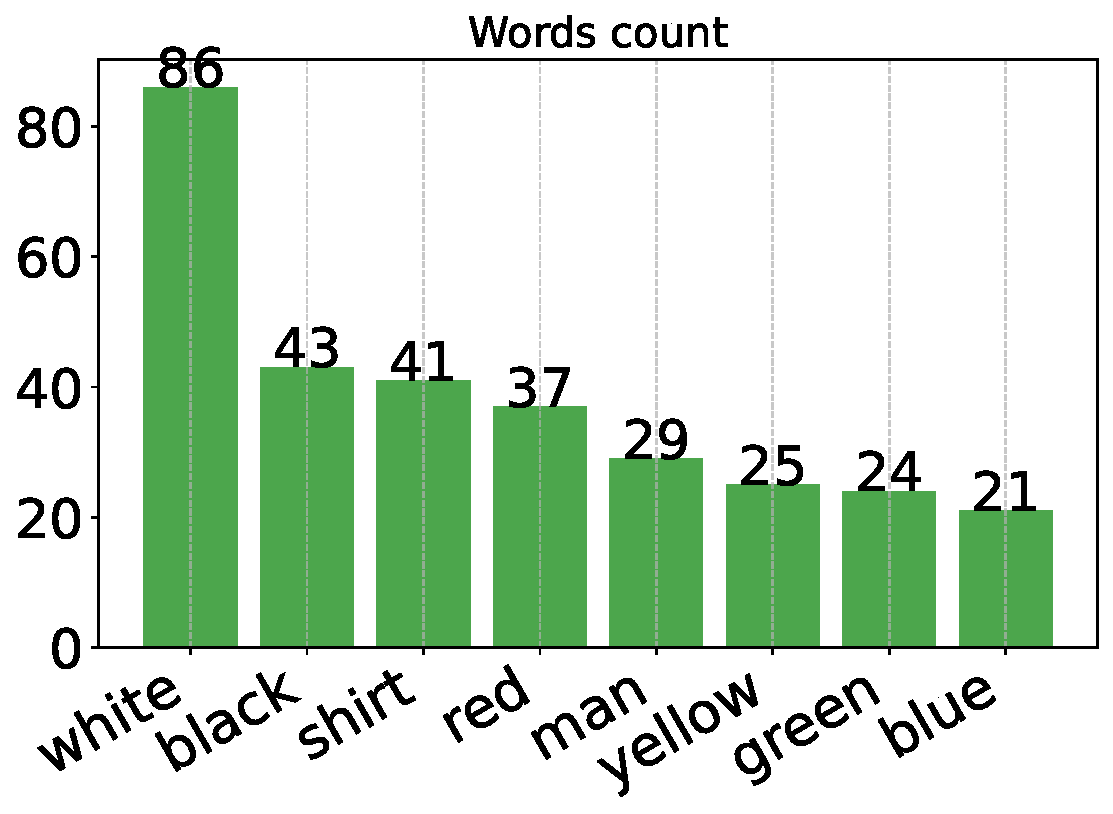
\includegraphics[width=1.0\textwidth]{Figures/model_steering/intra/coco/captioning_metrics_intra_llava_19_colors_onlytoi_steering_vector_concept_0_to_3_d_1000_ntcon_1.pdf}
        \end{minipage}%
        
        \begin{minipage}{0.24\linewidth}
            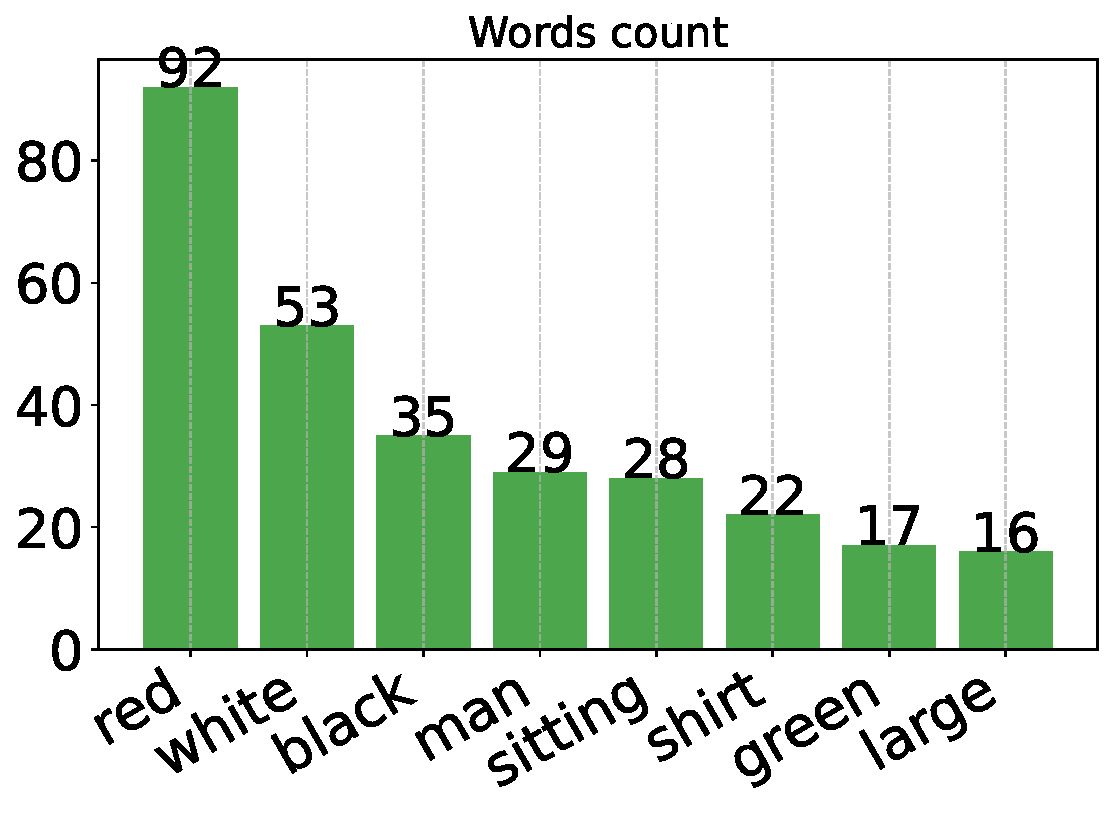
\includegraphics[width=1.0\textwidth]{Figures/model_steering/intra/coco/captioning_metrics_intra_llava_19_colors_onlytoi_steering_vector_concept_0_to_4_d_1000_ntcon_1.pdf}
        \end{minipage}%
        \begin{minipage}{0.24\linewidth}
            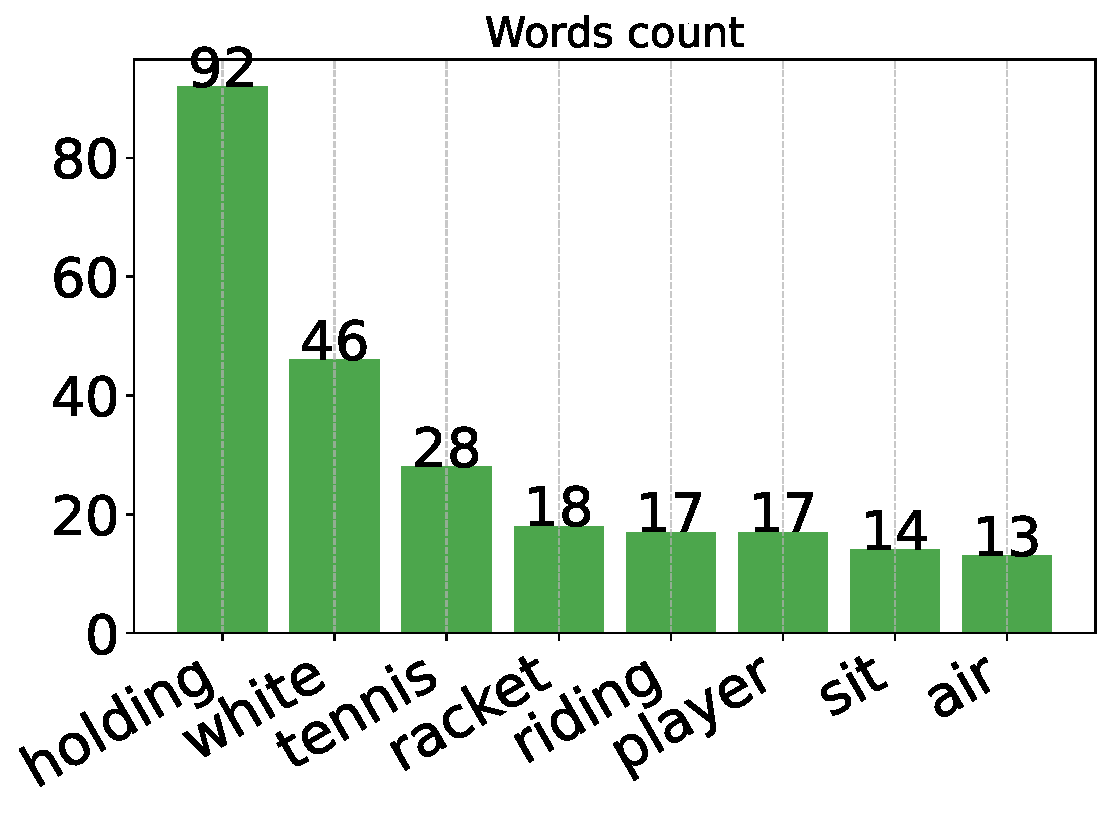
\includegraphics[width=1.0\textwidth]{Figures/model_steering/intra/coco/captioning_metrics_intra_llava_19_positive_sentiments_onlytoi_steering_vector_concept_0_to_2_d_1000_ntcon_1.pdf}
        \end{minipage}%
        \begin{minipage}{0.24\linewidth}
            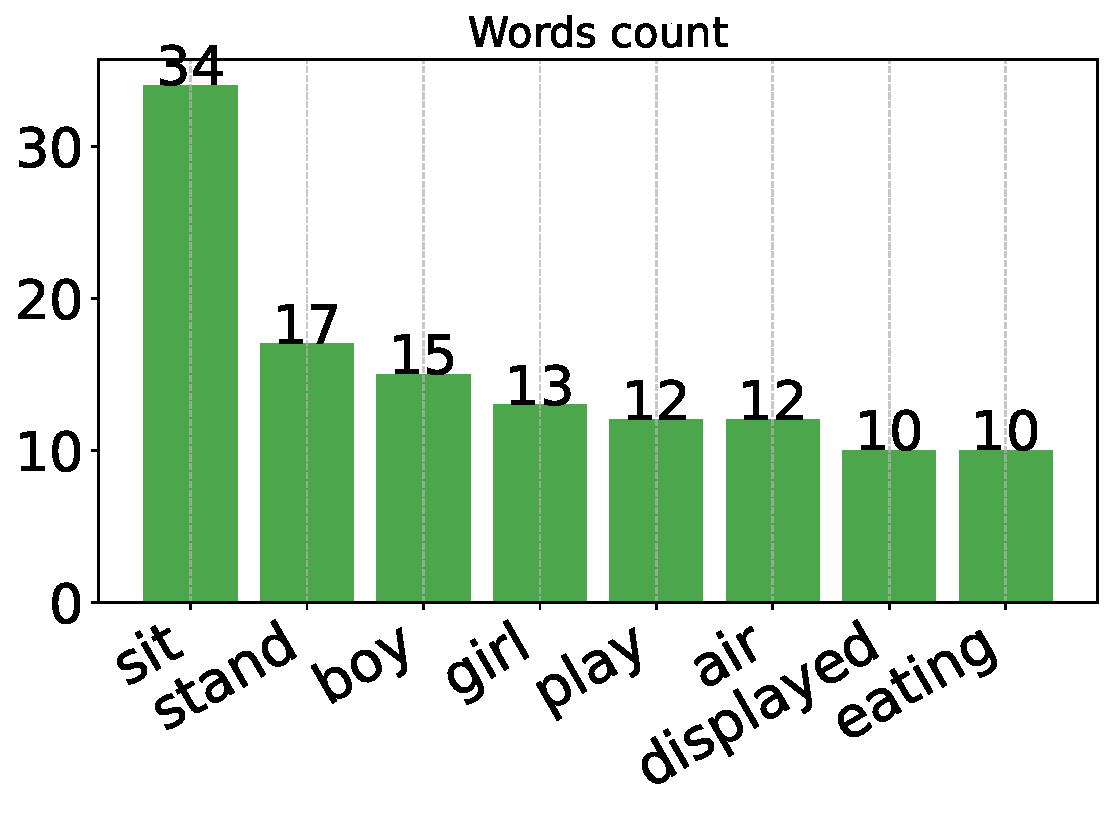
\includegraphics[width=1.0\textwidth]{Figures/model_steering/intra/coco/captioning_metrics_intra_llava_19_positive_sentiments_onlytoi_steering_vector_concept_0_to_5_d_1000_ntcon_1.pdf}
        \end{minipage}%
        \begin{minipage}{0.24\linewidth}
            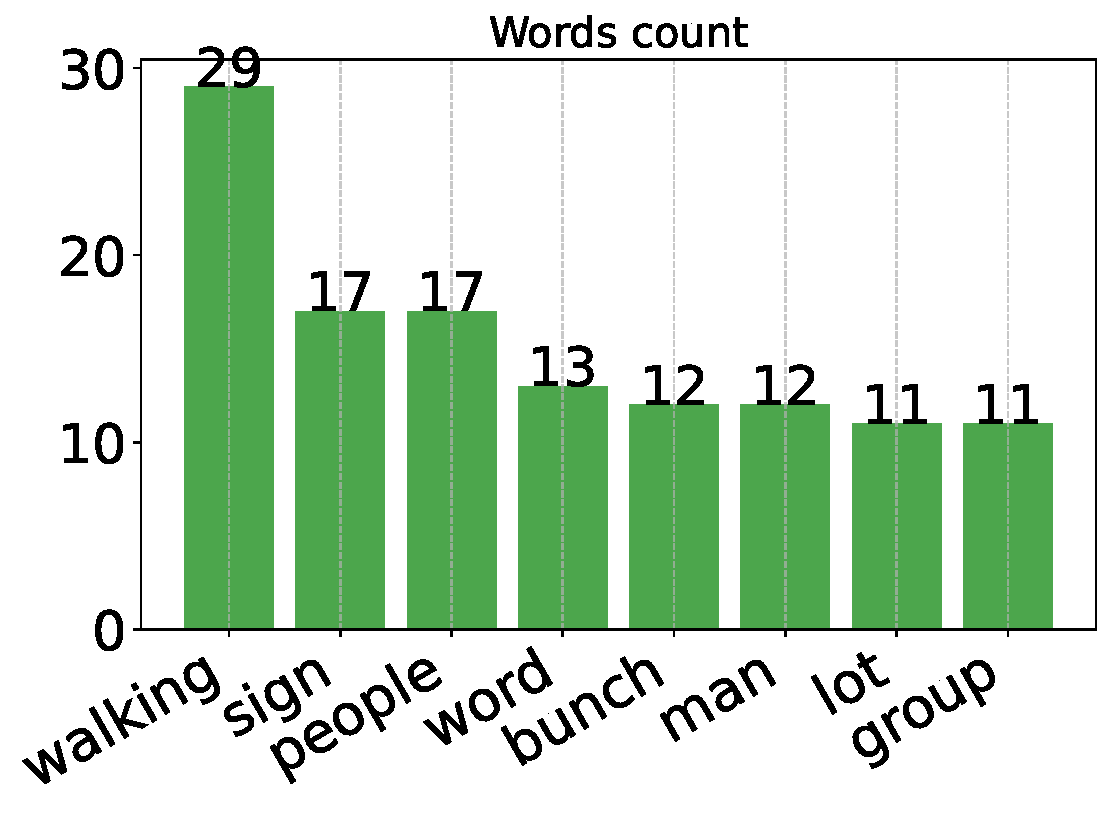
\includegraphics[width=1.0\textwidth]{Figures/model_steering/intra/coco/captioning_metrics_intra_llava_19_positive_sentiments_onlytoi_steering_vector_concept_0_to_6_d_1000_ntcon_1.pdf}
        \end{minipage}%
        
    \end{minipage}%
\caption{\textbf{Discovering meaningful steering directions with image captioning.} We report the relative increase in number of words counts. Each figure corresponds to different fine-grained steering direction.}
\label{fig:app_model_steering_intra_coco}
\end{figure*}





\begin{figure*}[!h]
    \centering
    \begin{minipage}{0.9\linewidth}
    \centering
        \begin{minipage}{0.24\linewidth}
            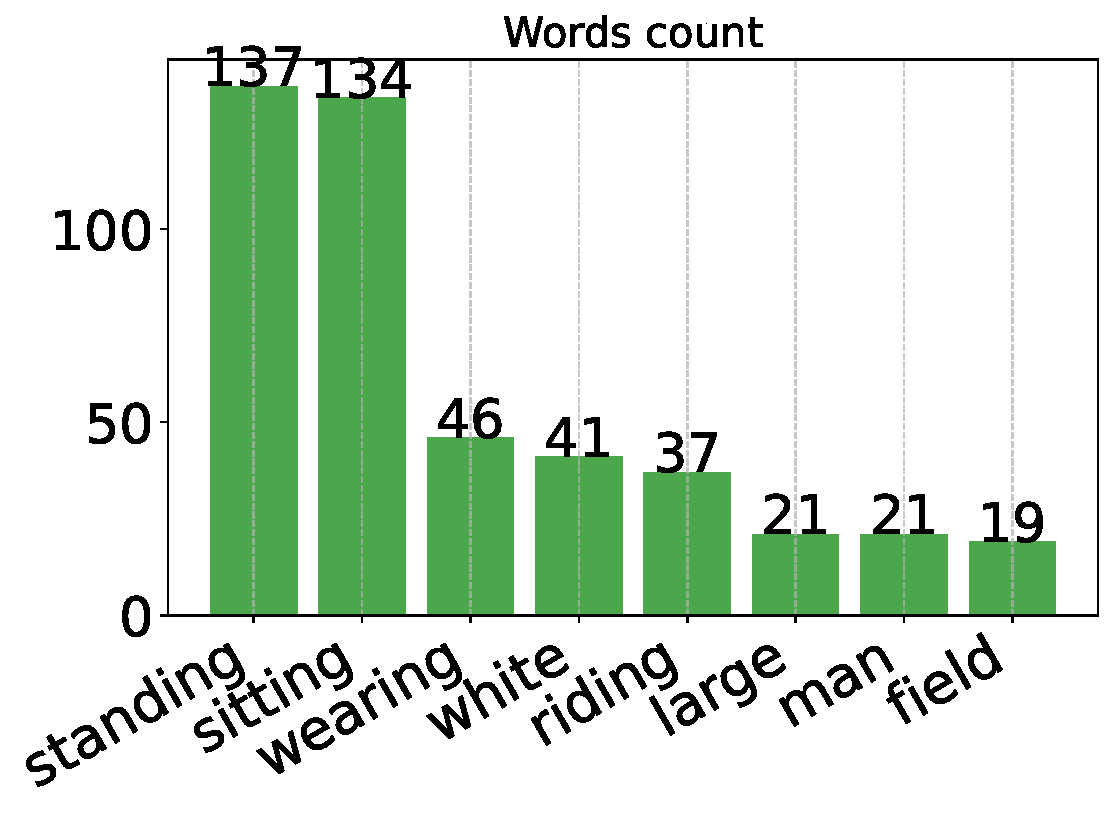
\includegraphics[width=1.0\textwidth]{Figures/model_steering/intra/coco/captioning_metrics_intra_llava_19_places_onlytoi_steering_vector_concept_0_to_2_d_1000_ntcon_3.pdf}
        \end{minipage}%
        \begin{minipage}{0.24\linewidth}
            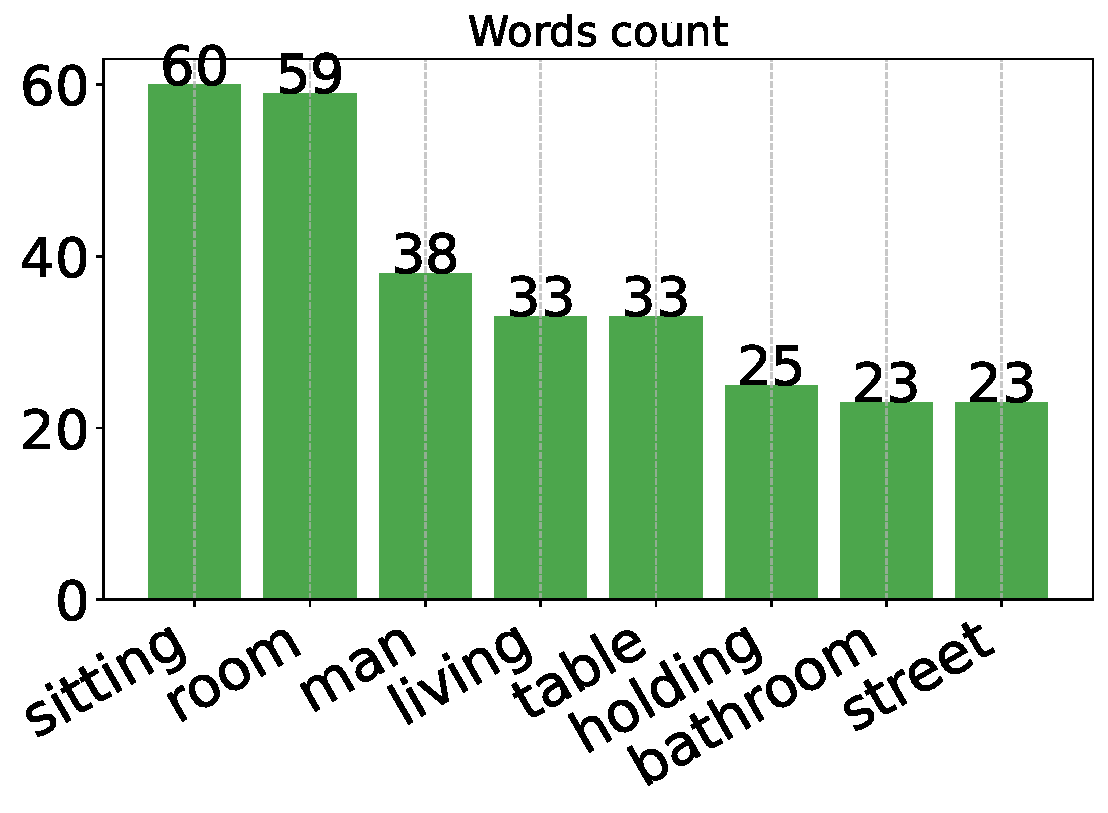
\includegraphics[width=1.0\textwidth]{Figures/model_steering/intra/coco/captioning_metrics_intra_llava_19_places_onlytoi_steering_vector_concept_0_to_8_d_1000_ntcon_3.pdf}
        \end{minipage}%
        \begin{minipage}{0.24\linewidth}
            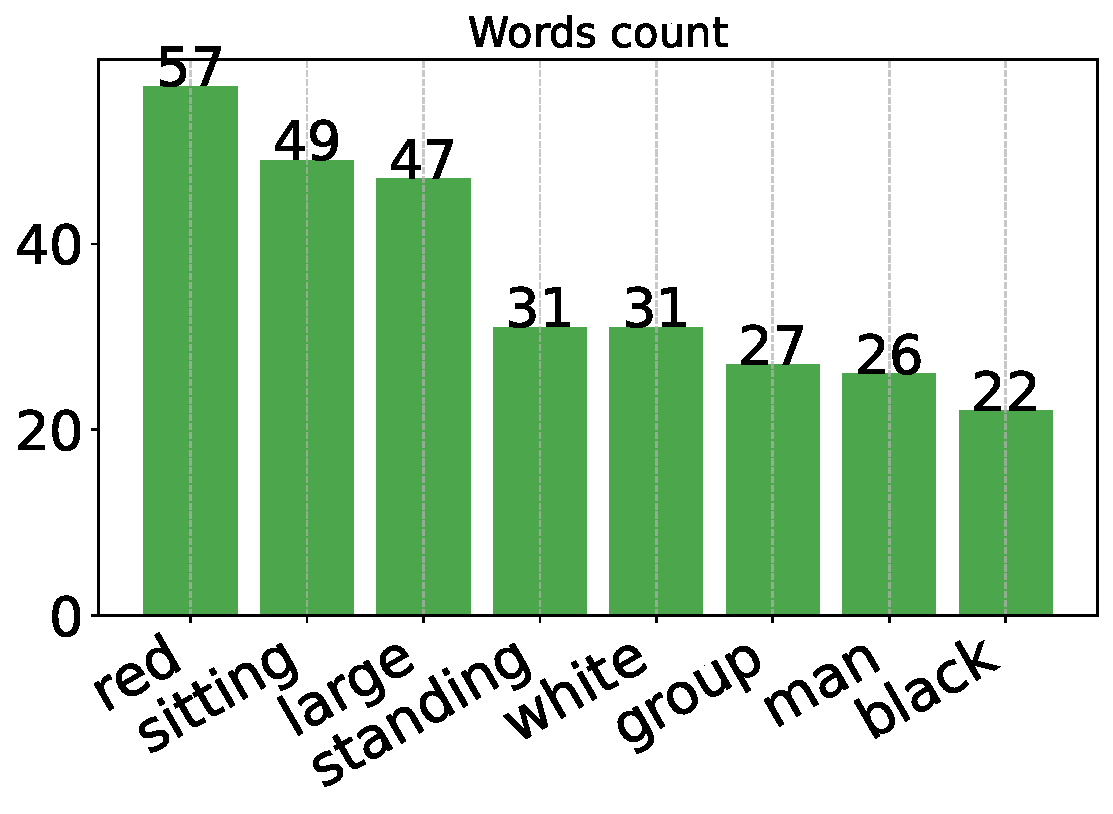
\includegraphics[width=1.0\textwidth]{Figures/model_steering/intra/coco/captioning_metrics_intra_llava_19_colors_onlytoi_steering_vector_concept_0_to_8_d_1000_ntcon_3.pdf}
        \end{minipage}%
        \begin{minipage}{0.24\linewidth}
            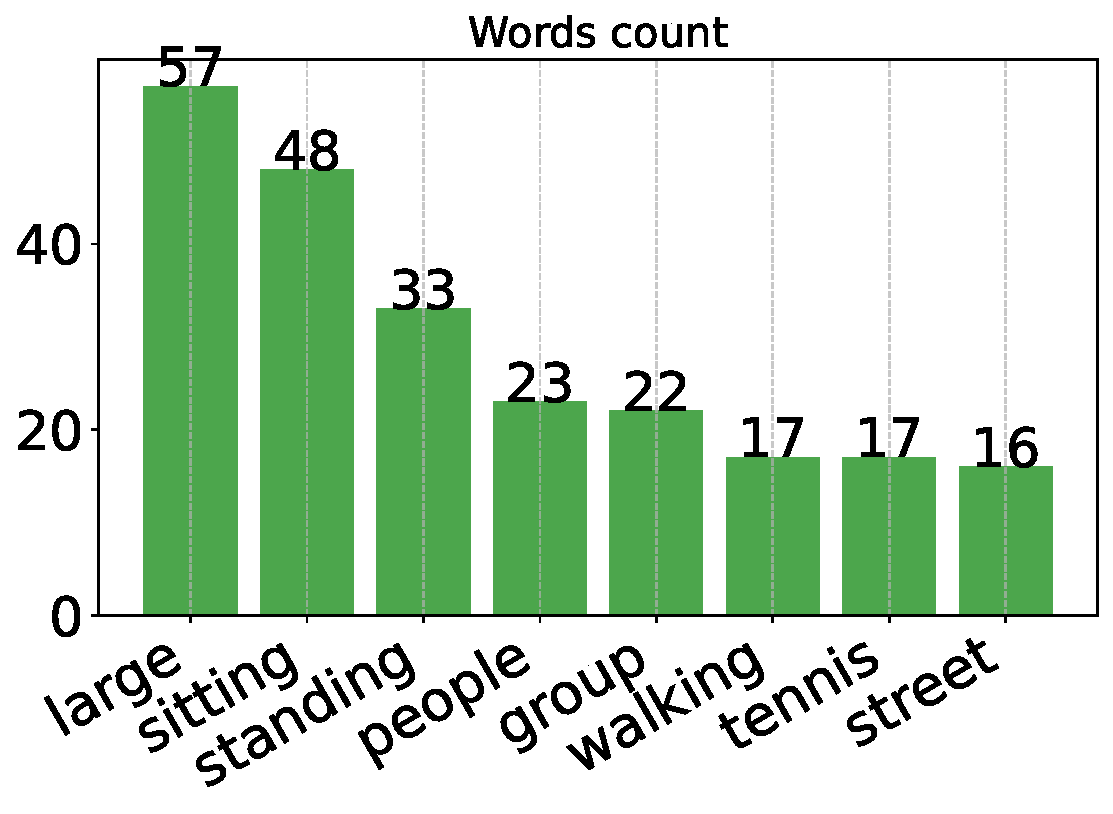
\includegraphics[width=1.0\textwidth]{Figures/model_steering/intra/coco/captioning_metrics_intra_llava_19_colors_onlytoi_steering_vector_concept_0_to_9_d_1000_ntcon_3.pdf}
        \end{minipage}%
        
        \begin{minipage}{0.24\linewidth}
            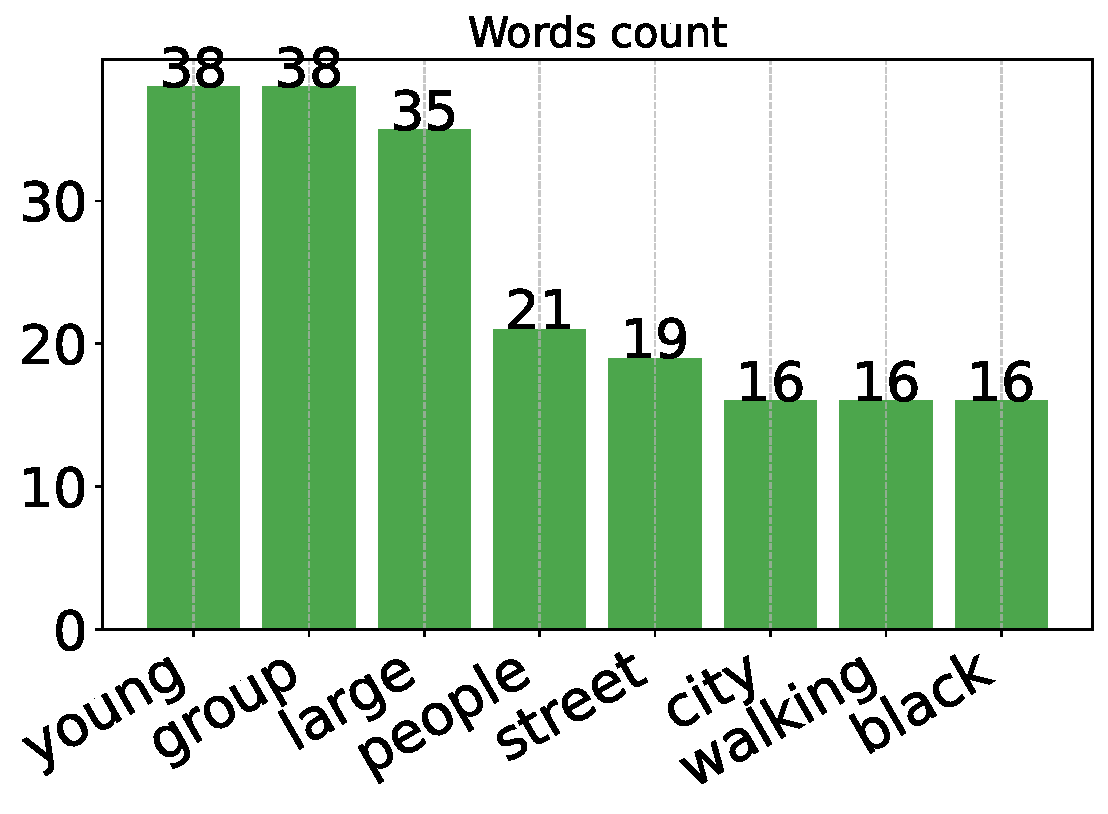
\includegraphics[width=1.0\textwidth]{Figures/model_steering/intra/coco/captioning_metrics_intra_llava_19_colors_onlytoi_steering_vector_concept_1_to_2_d_1000_ntcon_3.pdf}
        \end{minipage}%
        \begin{minipage}{0.24\linewidth}
            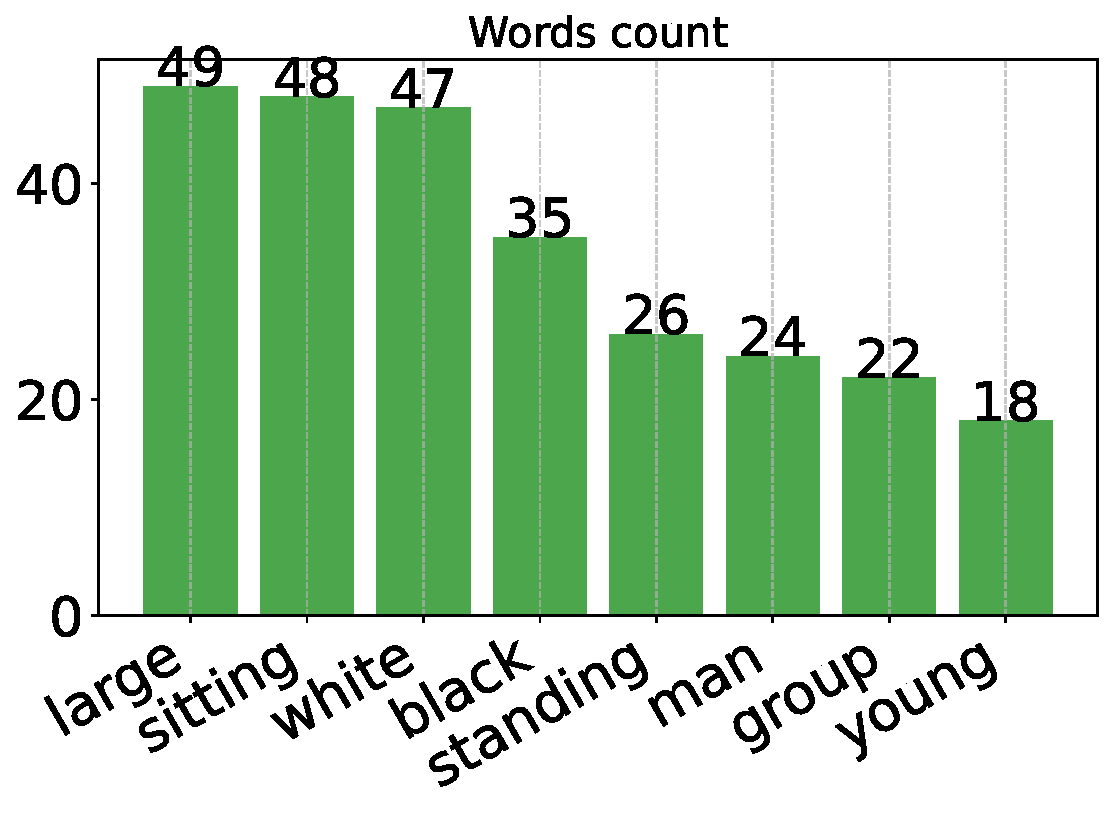
\includegraphics[width=1.0\textwidth]{Figures/model_steering/intra/coco/captioning_metrics_intra_llava_19_colors_onlytoi_steering_vector_concept_1_to_3_d_1000_ntcon_3.pdf}
        \end{minipage}%
        \begin{minipage}{0.24\linewidth}
            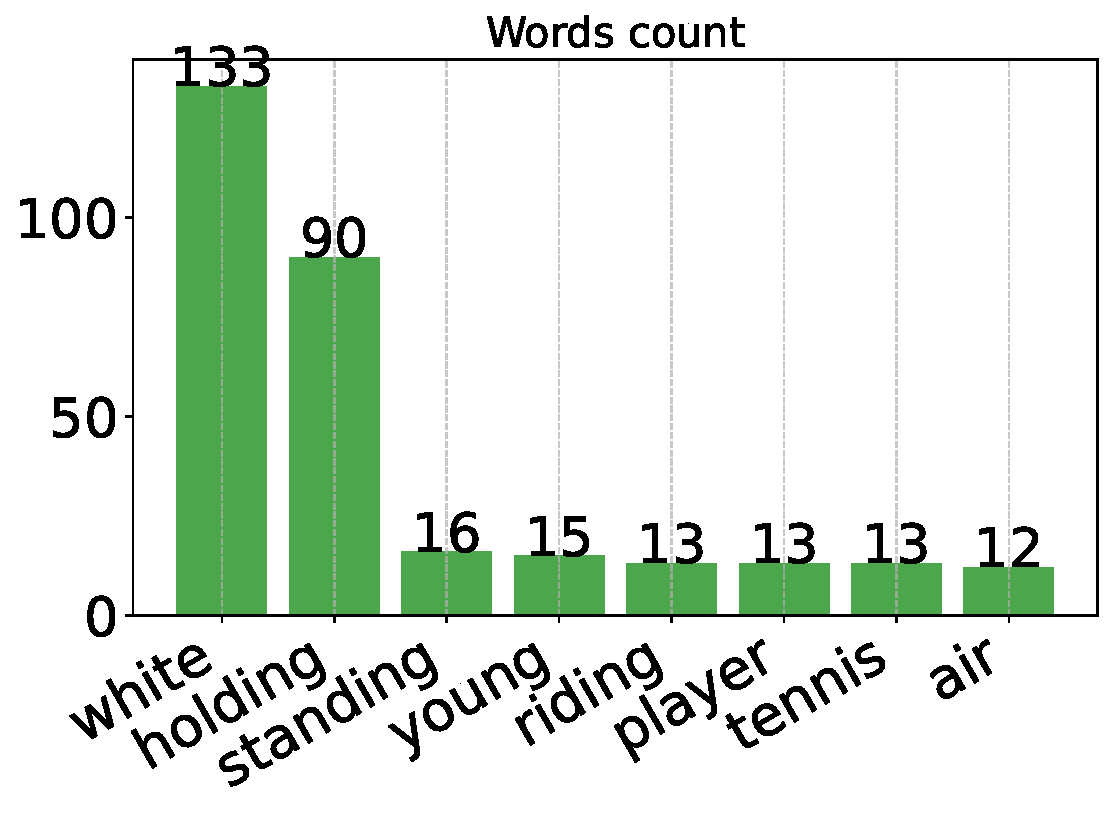
\includegraphics[width=1.0\textwidth]{Figures/model_steering/intra/coco/captioning_metrics_intra_llava_19_positive_sentiments_onlytoi_steering_vector_concept_0_to_4_d_1000_ntcon_3.pdf}
        \end{minipage}%
        \begin{minipage}{0.24\linewidth}
            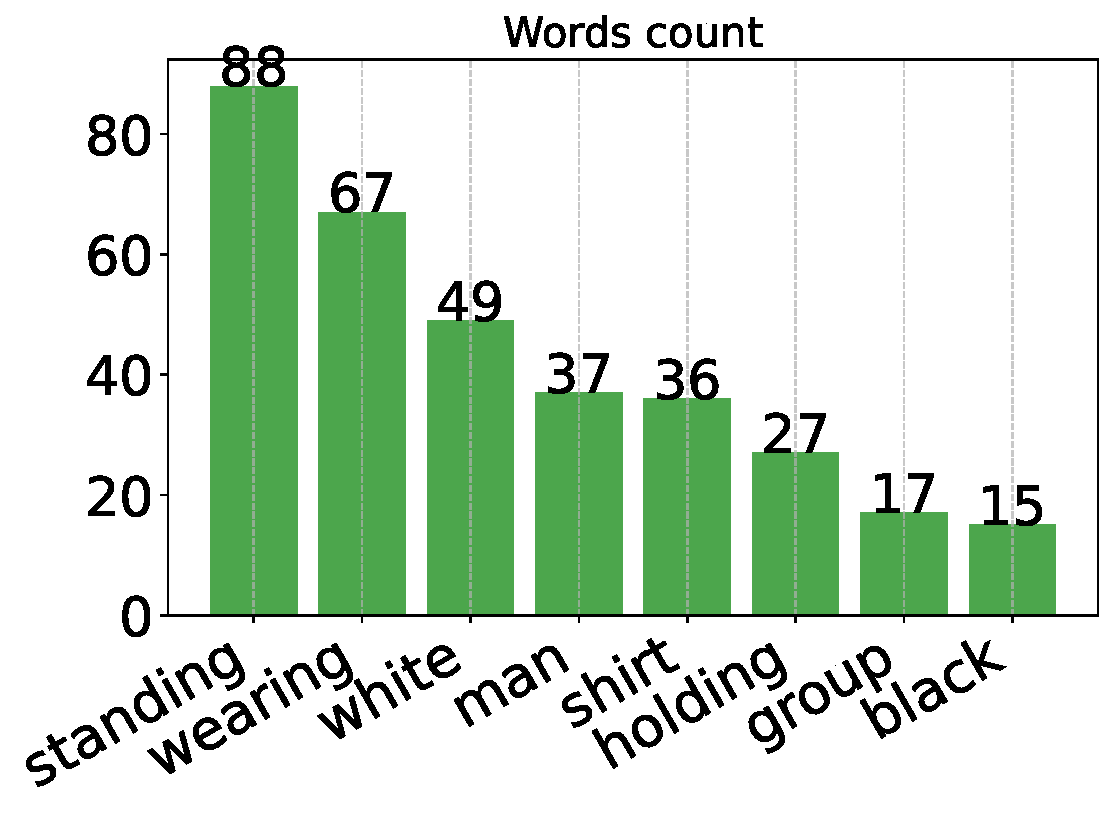
\includegraphics[width=1.0\textwidth]{Figures/model_steering/intra/coco/captioning_metrics_intra_llava_19_positive_sentiments_onlytoi_steering_vector_concept_1_to_4_d_1000_ntcon_3.pdf}
        \end{minipage}%
         
    \end{minipage}%
\caption{\textbf{Discovering meaningful steering directions with image captioning towards multiple concepts.} We report the relative increase in number of words count. Each figure corresponds to different fine-grained steering direction towards multiple concepts.}
\label{fig:app_model_steering_intra_coco_multi}
\end{figure*}



\subsection{Steering image captions.}
\label{sec:app_image_captions}

Similar to VQAv2, we extract the concepts from a set of image captions and compute the steering vectors between each pair of concepts. \Cref{fig:app_model_steering_intra_coco} illustrate some of these vectors. Based on the relative increase in words count, we can notice that some steering vectors are related to specific concepts, such as "holding" or "black". In addition, we find (\Cref{fig:app_model_steering_intra_coco_multi}) some vectors correspond to multiple concepts, such as "standing" and "sitting" or "young" and "group" and "large".






\subsection{Ablation study}
\label{sec:app_model_steering_ablation_study}
In this section, we ablate several steering design choices.


\begin{figure*}[t]
    \centering
    \begin{minipage}{0.8\linewidth}
    \centering
        \begin{minipage}{\linewidth}
            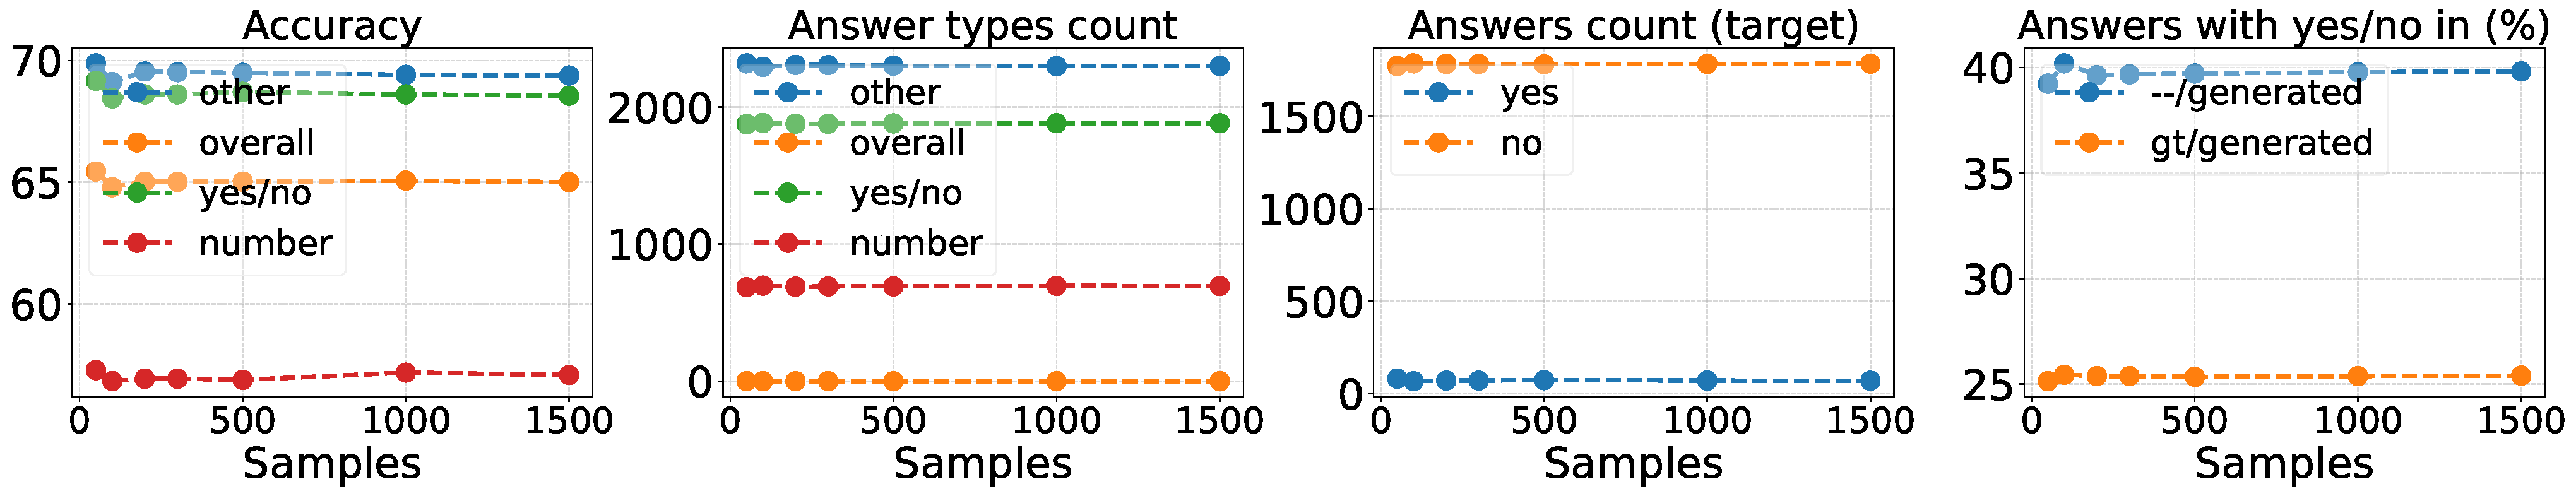
\includegraphics[width=1.0\textwidth]{Figures/model_steering/ablate_samples/model_steering_shift_of_means_ablate_token_of_interest_num_samples_yes_to_no_mini.pdf}
        \end{minipage}%
        
        \begin{minipage}{\linewidth}
            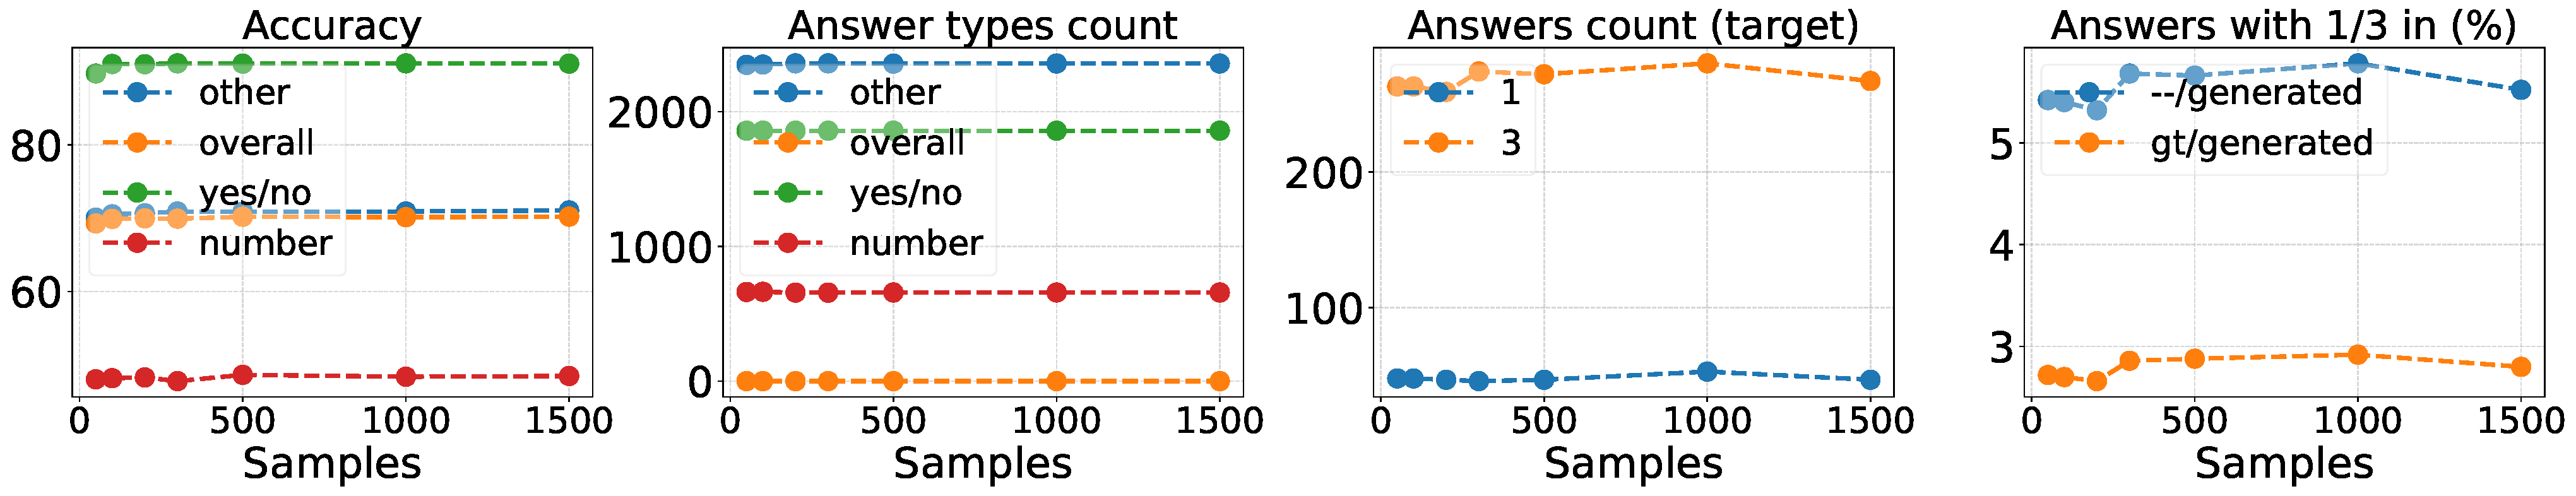
\includegraphics[width=1.0\textwidth]{Figures/model_steering/ablate_samples/model_steering_shift_of_means_ablate_token_of_interest_num_samples_1_to_3_mini.pdf}
        \end{minipage}%
        
        \begin{minipage}{\linewidth}
            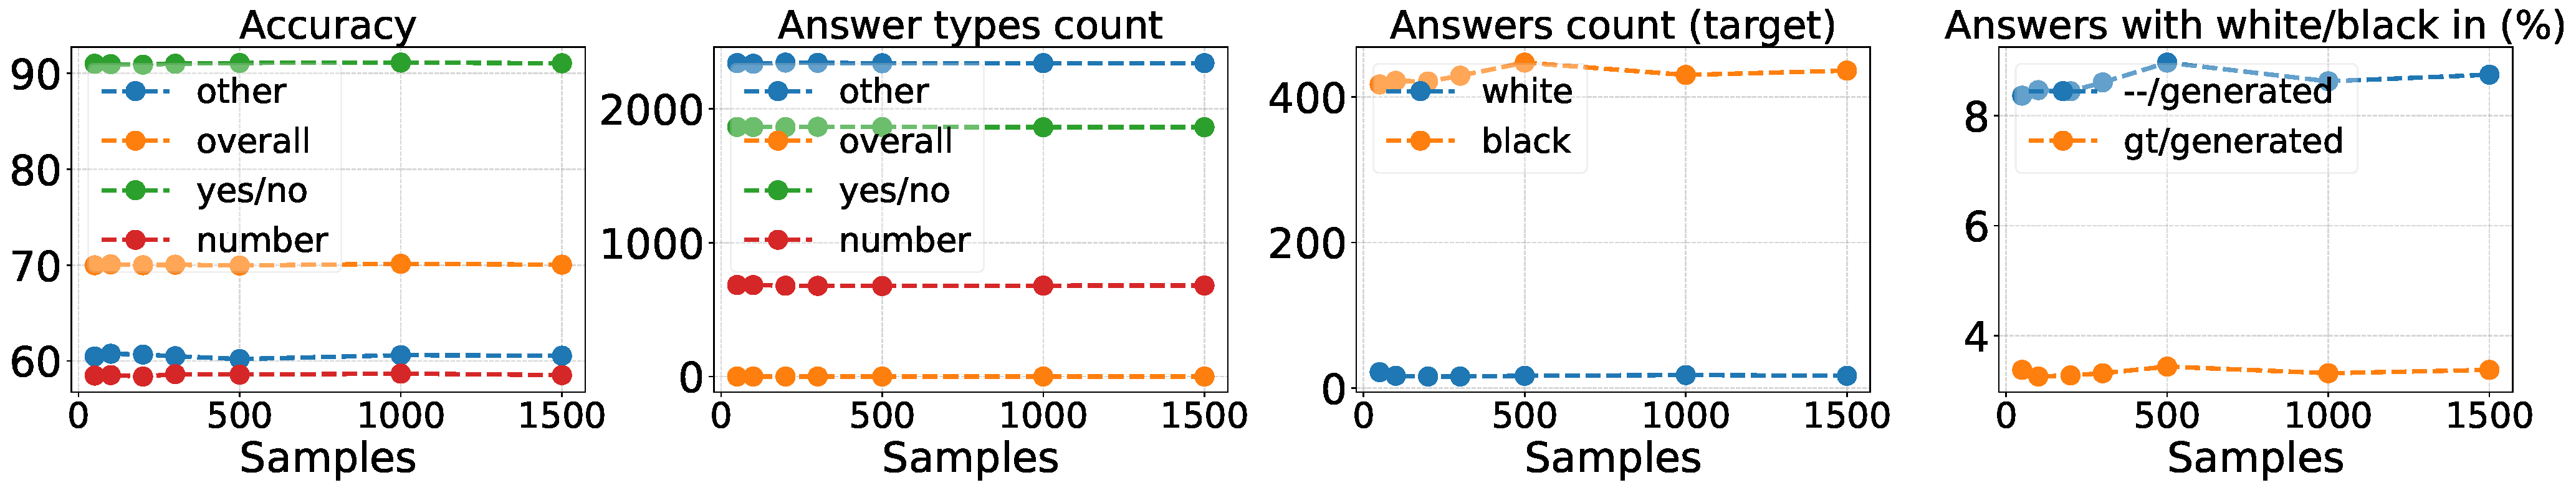
\includegraphics[width=1.0\textwidth]{Figures/model_steering/ablate_samples/model_steering_shift_of_means_ablate_token_of_interest_num_samples_white_to_black_mini.pdf}
        \end{minipage}%
    
    \end{minipage}%
\caption{\textbf{Ablation study: number of samples to compute steering vector.} From top to bottom: steering answers from "Yes" (yes/no), "1" (number), "White" (other) to "No", "3", "Black" respectively. We report different metrics as follows (from left to right): VQA accuracy per answer type, number of answers belonging to each type, number of occurrence of the original and target answers (\emph{e.g.}, yes and no), number of answers that contain the target answers (--/generated) and in addition the original answer in the ground truth (gt/generated). Computing the steering vector is robust to varying the number of samples.}
\label{fig:model_steering_ablate_samnples}
\end{figure*}



\begin{figure}[t]
    \centering
    \begin{minipage}{\linewidth}
    \centering
        \begin{minipage}{\linewidth}
            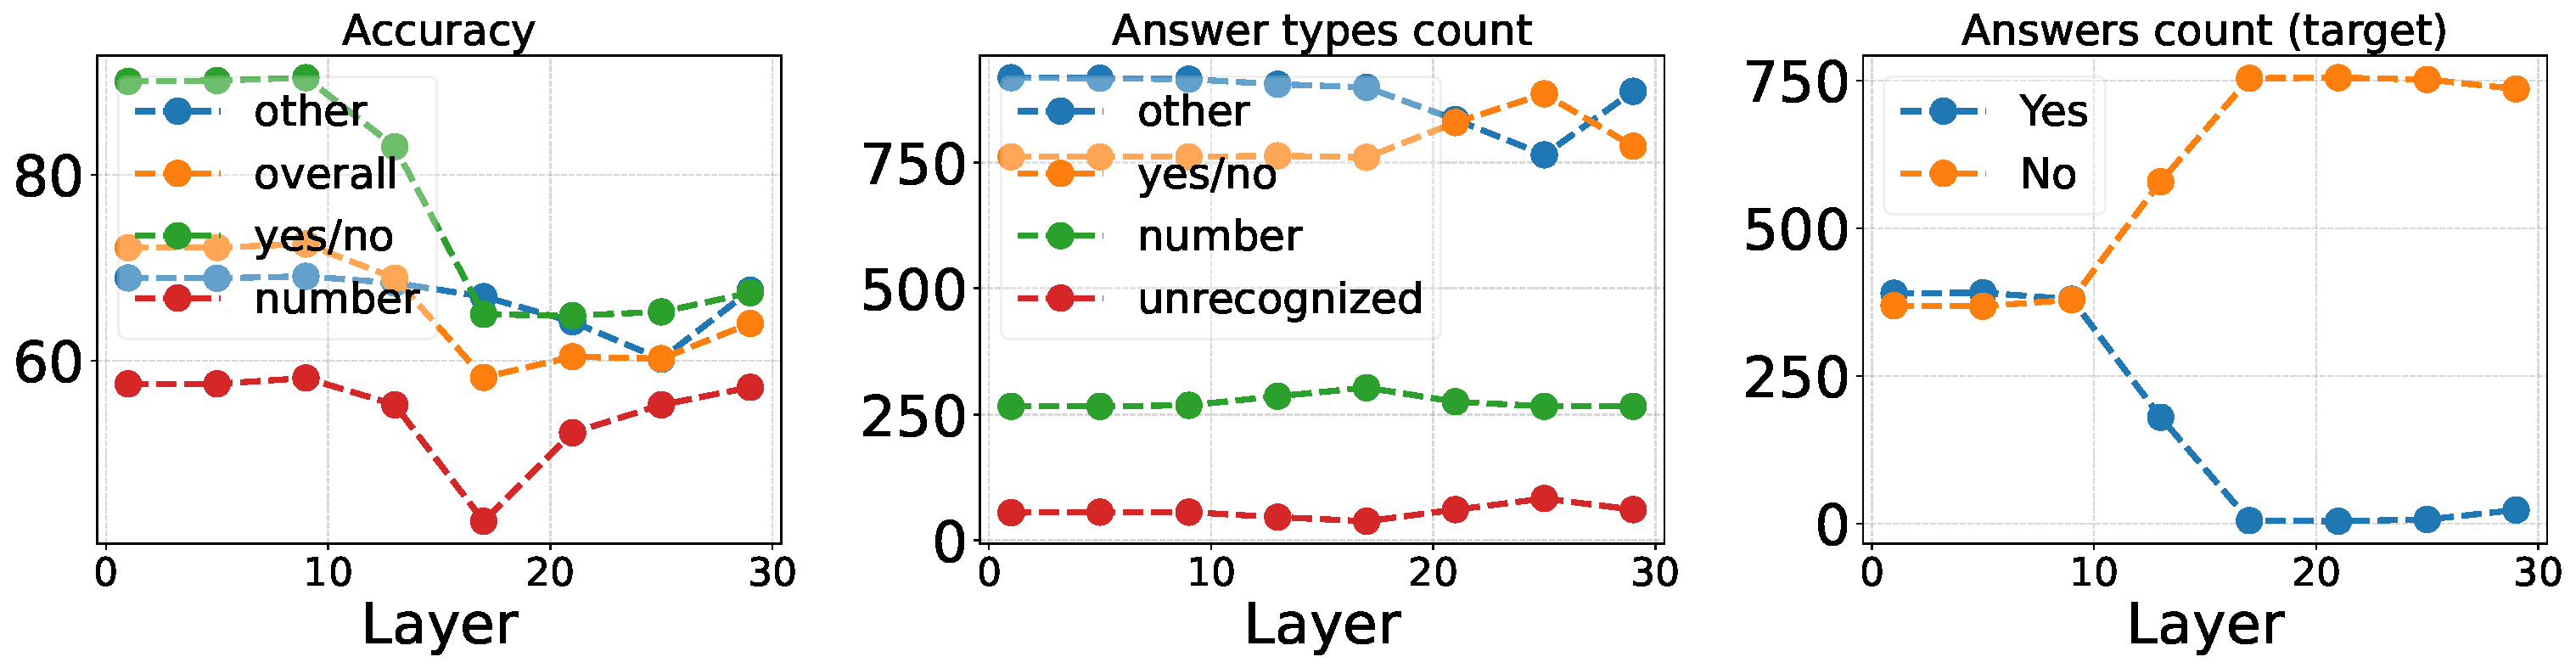
\includegraphics[width=1.0\textwidth]{Figures/model_steering/ablate_layers/model_steering_ablate_layers_yes_to_no.pdf}
        \end{minipage}%
        
        \begin{minipage}{\linewidth}
            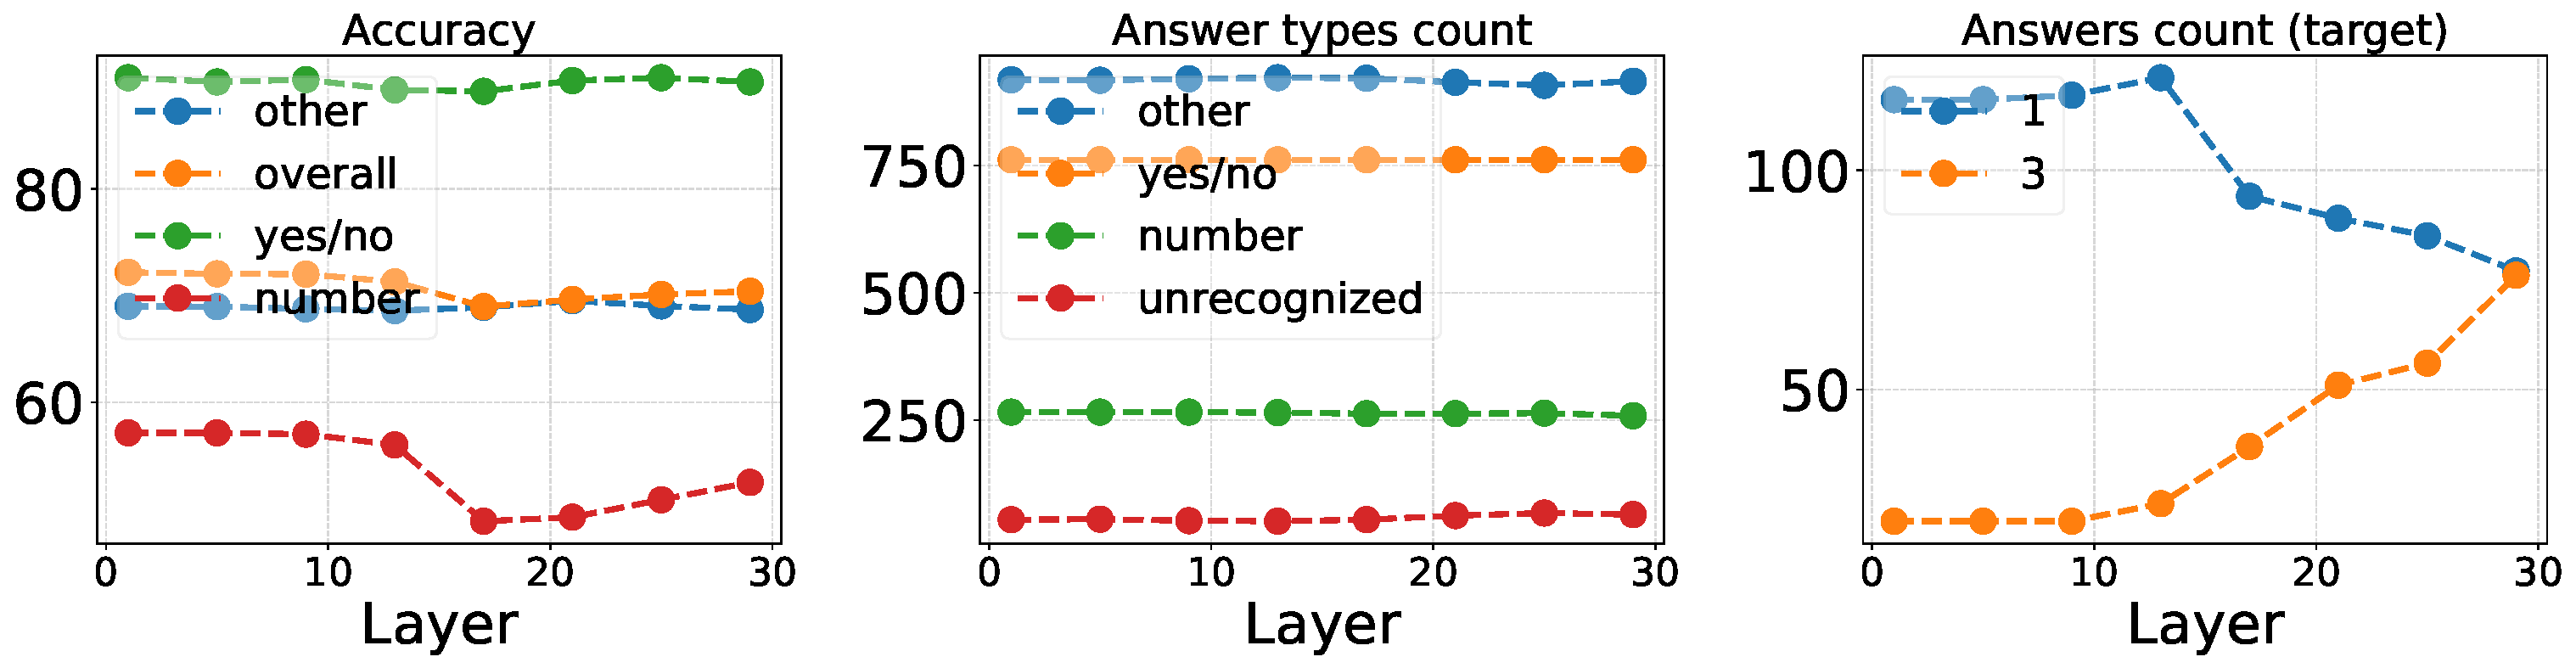
\includegraphics[width=1.0\textwidth]{Figures/model_steering/ablate_layers/model_steering_ablate_layers_1_to_3.pdf}
        \end{minipage}%
        
        \begin{minipage}{\linewidth}
            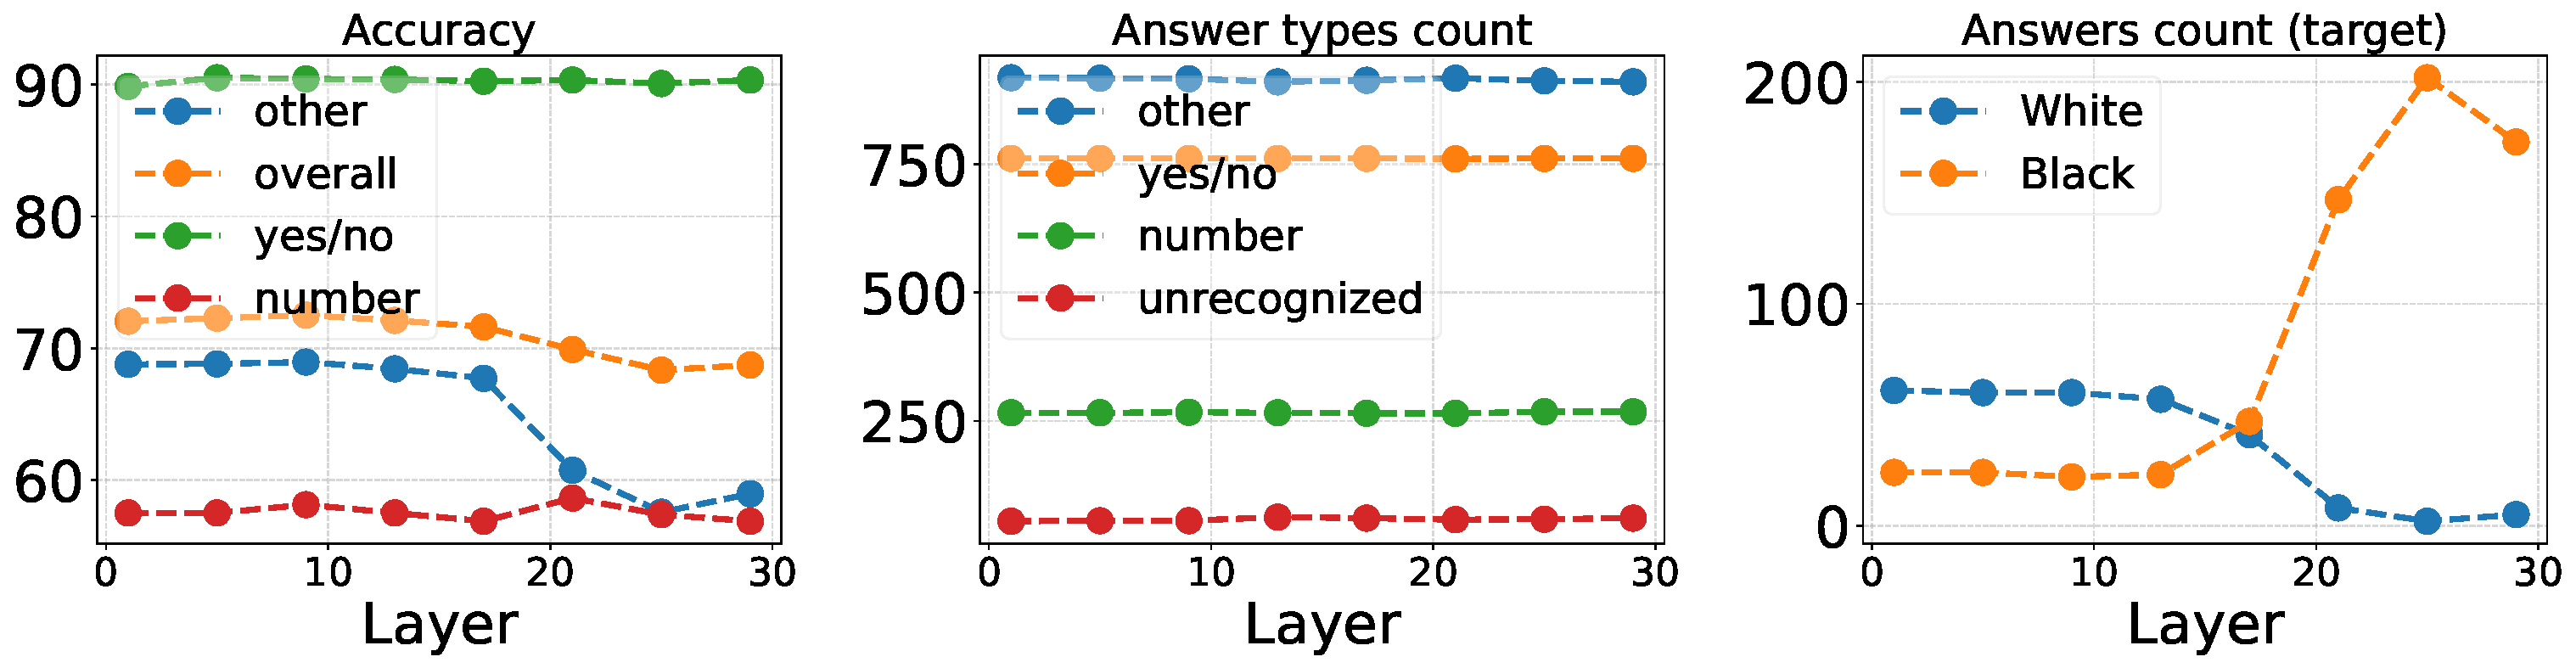
\includegraphics[width=1.0\textwidth]{Figures/model_steering/ablate_layers/model_steering_ablate_layers_white_to_black.pdf}
        \end{minipage}%
    
    \end{minipage}%
\caption{\textbf{Ablation study: steering MLLMs across layers.} From top to bottom, steering answers from: "Yes" (yes/no), "1" (number), "White" (other) to "No", "3", "Black" respectively. Steering is more effective in deeper layers as the number of original/target answer counts decrease/increase significantly. In last layers, the accuracy on other answers type changes slightly, and the number of answers types count remains almost constant.}
\label{fig:model_steering_ablate_layers}
\end{figure}



\subsubsection{Number of samples}
\label{sec:app_model_steering_ablate_num_samples}

An interesting question to ask is how the steering is affected by the number of samples. To provide an answer, we vary the number of samples (\emph{e.g.} answers with yes and no) used to compute the steering vectors and report the results in \Cref{fig:model_steering_ablate_samnples}. Interestingly, the steering is effective even with very few samples (\emph{e.g.}, 50) and it is robust to the number of samples, where the scores start to saturate after 500 samples. This reveals that steering could be a good data-efficient solution for setups with very little data.




\subsubsection{Steering layer}
\label{sec:app_ablate_layers}

We apply the steering to a specific layer inside the LLM, where the steering vector is computed using the output activations of the same layer. \Cref{fig:model_steering_ablate_layers} shows that the steering is more effective in deeper layers. For instance, the number of original/target answers decrease/increase significantly while the accuracy on other answer types remains unchanged (layer 0 is considered the baseline).







\begin{figure*}[t]
    \centering
    \begin{minipage}{0.8\linewidth}
    \centering
        \begin{minipage}{\linewidth}
            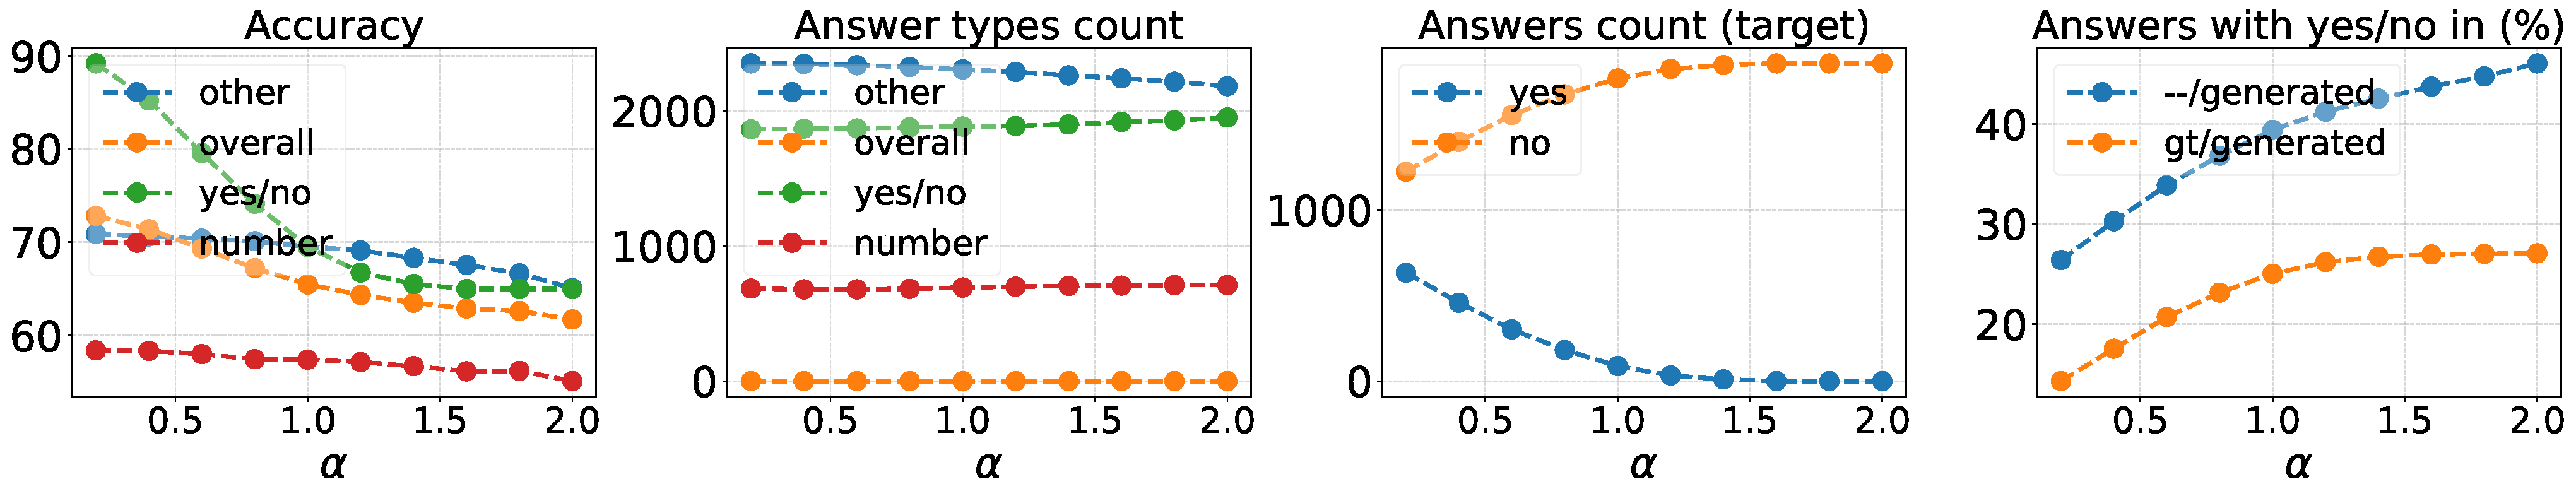
\includegraphics[width=1.0\textwidth]{Figures/model_steering/ablate_alpha/model_steering_shift_of_means_ablate_alpha_yes_to_no_mini.pdf}
        \end{minipage}%
        
        \begin{minipage}{\linewidth}
            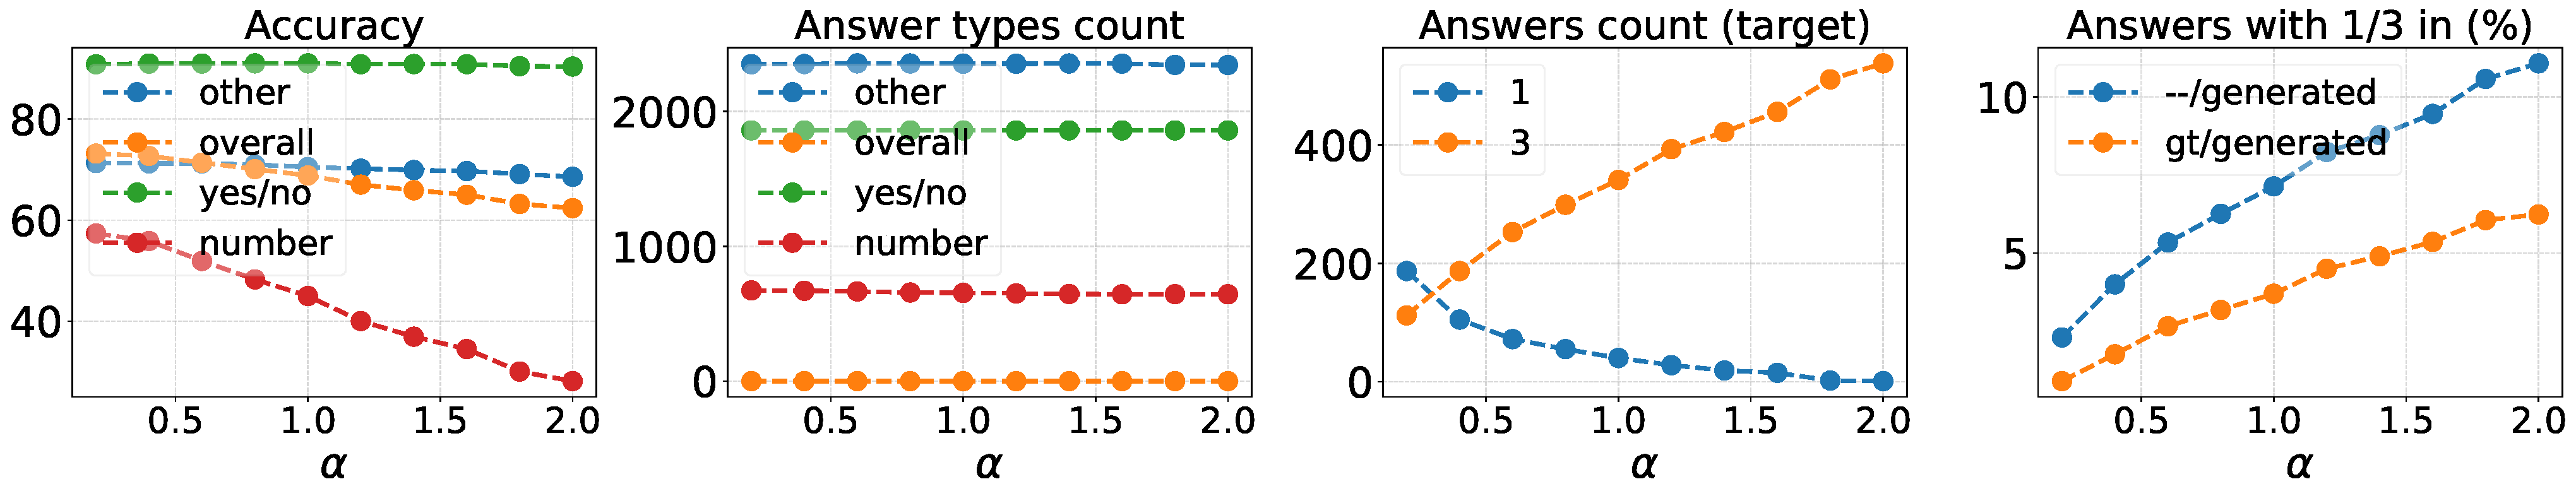
\includegraphics[width=1.0\textwidth]{Figures/model_steering/ablate_alpha/model_steering_shift_of_means_ablate_alpha_1_to_3_mini.pdf}
        \end{minipage}%
        
        \begin{minipage}{\linewidth}
            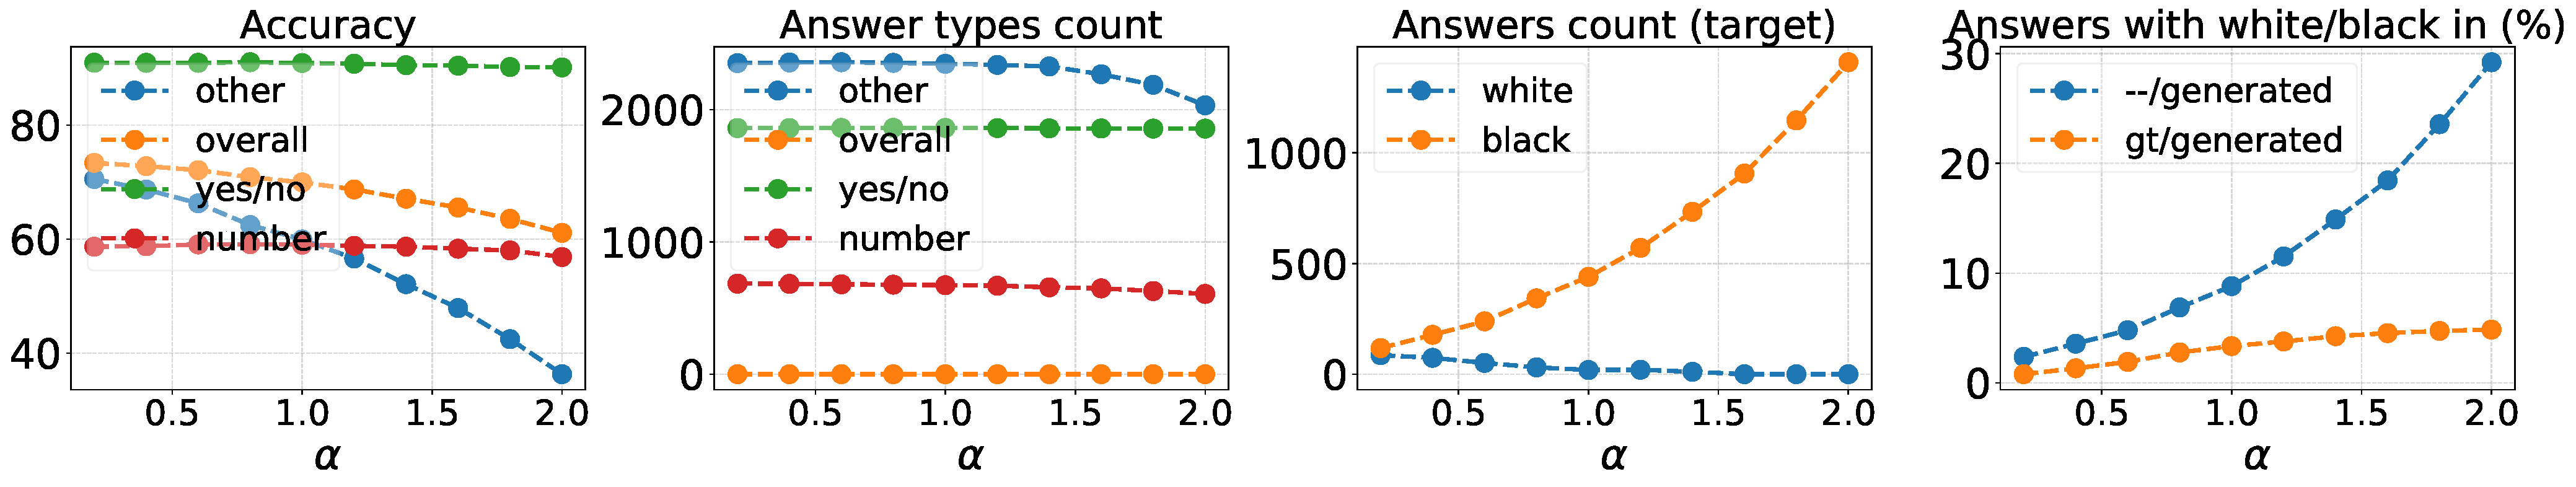
\includegraphics[width=1.0\textwidth]{Figures/model_steering/ablate_alpha/model_steering_shift_of_means_ablate_alpha_white_to_black_mini.pdf}
        \end{minipage}%
    
    \end{minipage}%
\caption{\textbf{Ablation study: steering strength ($\alpha$).} From top to bottom: steering answers from "Yes" (yes/no), "1" (number), "White" (other) to "No", "3", "Black" respectively. We report different metrics as follows (from left to right): VQA accuracy per answer type, number of answers belonging to each type, number of occurrence of the original and target answers (\emph{e.g.}, yes and no), number of answers that contain the target answers (--/generated) and in addition the original answer in the ground truth (gt/generated). Increasing $\alpha$ pushes the model to generate more the target answer. However, the steering becomes less targeted, as seen in the last column.}
\label{fig:model_steering_ablate_alpha}
\end{figure*}


\subsubsection{Steering strength ($\alpha$)}
\label{sec:app_model_steering_ablate_alpha}

In this section, we study the effect of steering strength across different setups. In general, we find that increasing $\alpha$ leads to more steering effect. However, there is trade-off between the steering effect, targeted steering and the quality of the generated response. 

\paragraph{Steering MLLMs answers.} We steer the model to change an original answer towards a target one. \Cref{fig:model_steering_ablate_alpha} shows that increasing $\alpha$ pushes the model to generate the target answer more (as seen from the Answers count (target)). However, the steering becomes less targeted, as seen in the last column. For instance, the model starts generating the target answers even if the original answer is not included in the ground truth (gt/generated score).




\begin{figure}[t]
    \centering
    \begin{minipage}{1\linewidth}
    
        \begin{minipage}{0.32\linewidth} %
            \centering
            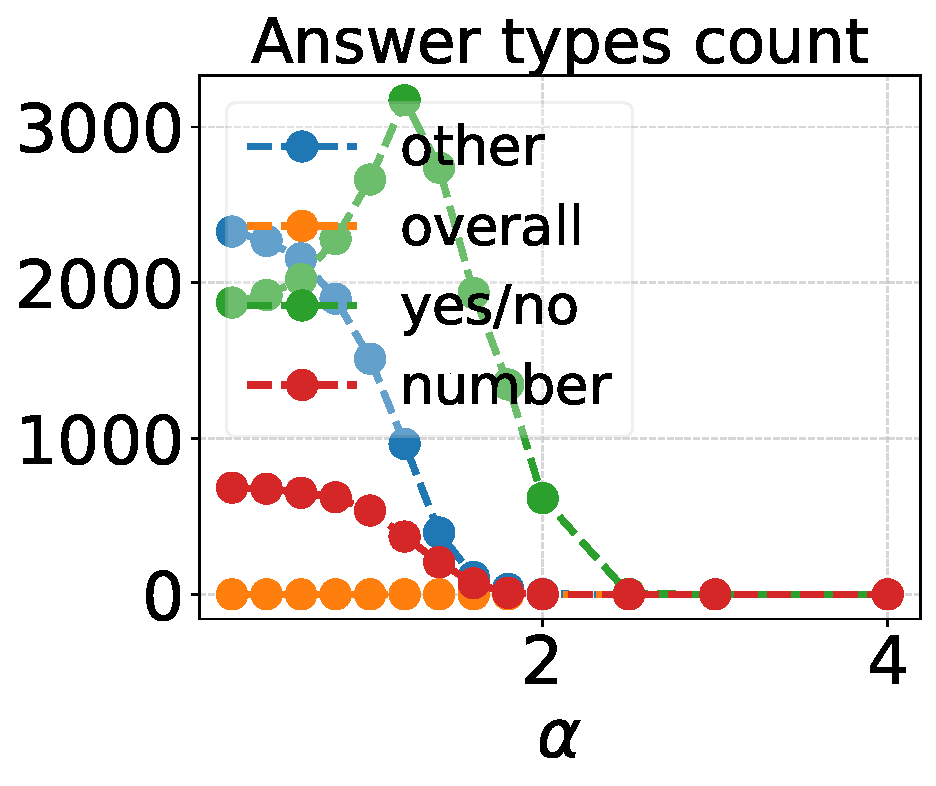
\includegraphics[width=\linewidth]{Figures/model_steering/ablate_alpha/answers_type/model_steering_shift_of_means_ablate_alpha_llava_type_yes_no_Answer_types_count.pdf}
        \end{minipage}%
        \begin{minipage}{0.32\linewidth} %
            \centering
            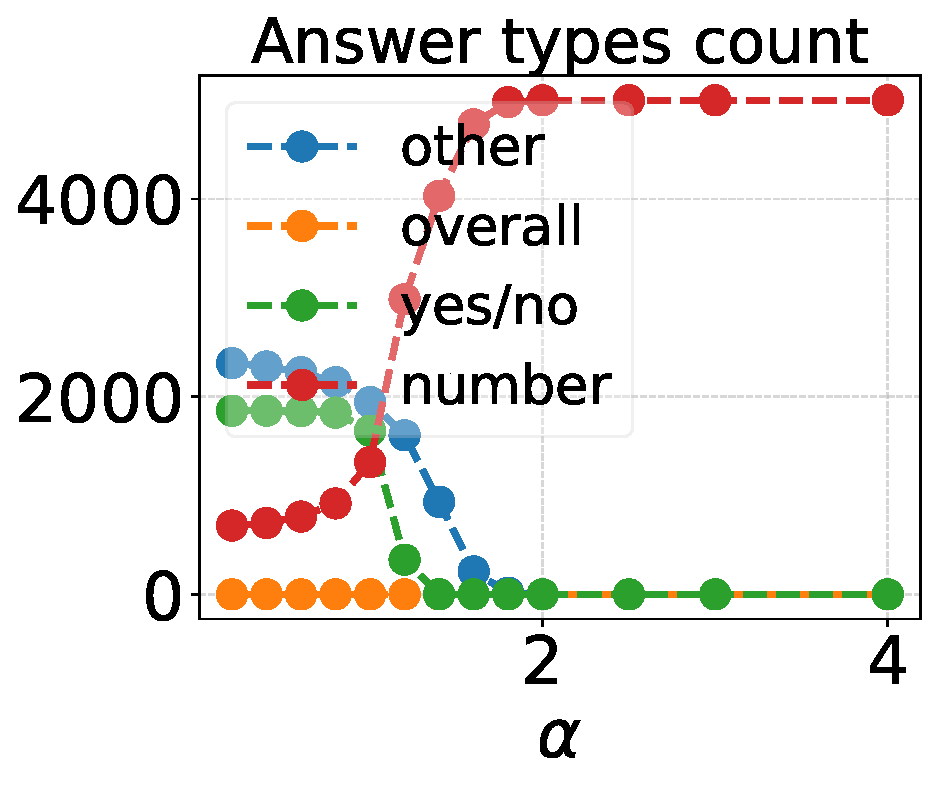
\includegraphics[width=\linewidth]{Figures/model_steering/ablate_alpha/answers_type/model_steering_shift_of_means_ablate_alpha_llava_type_number_Answer_types_count.pdf}
        \end{minipage}%
        \begin{minipage}{0.32\linewidth} %
            \centering
            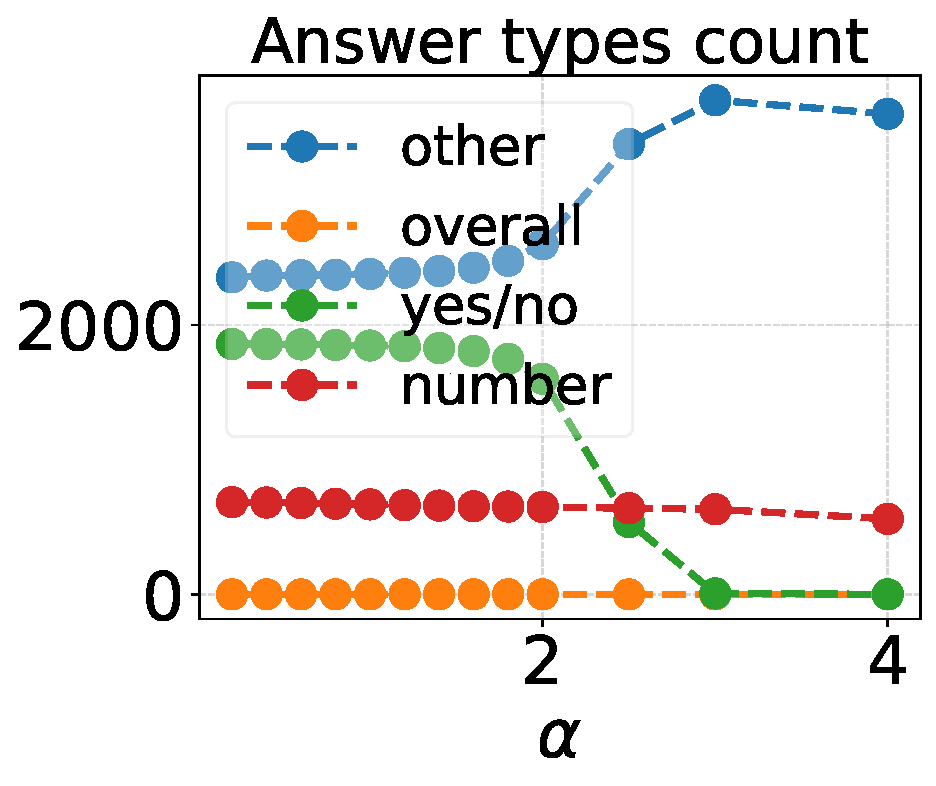
\includegraphics[width=\linewidth]{Figures/model_steering/ablate_alpha/answers_type/model_steering_shift_of_means_ablate_alpha_llava_type_other_Answer_types_count.pdf}
        \end{minipage}%


        
    \end{minipage}%


    \caption{\textbf{Ablation study: steering strength ($\alpha$) and changing answer types.} From left to right: steering answers type towards: yes/no, number and other. We report the number of answers in each answer type. Increasing $\alpha$ pushes the model to generate more answers from the target type.}
    \label{fig:model_steering_ablate_alpha_answers_type}
\end{figure}




\begin{figure}[t]
    \centering
    \begin{minipage}{1\linewidth}
    
        \begin{minipage}{0.32\linewidth} %
            \centering
            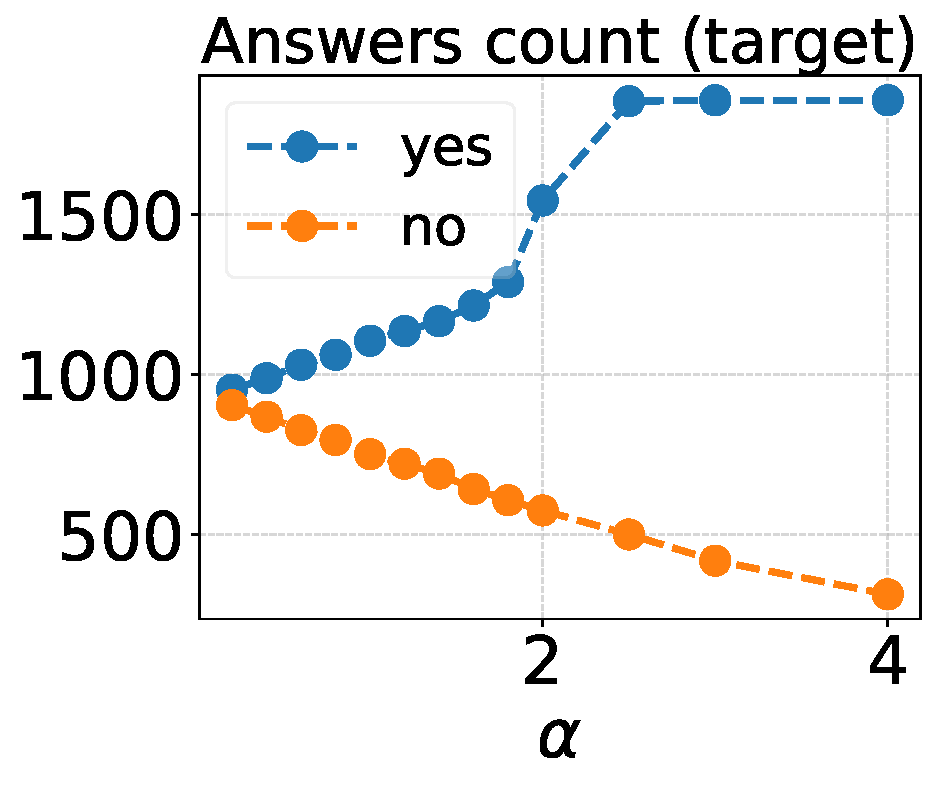
\includegraphics[width=\linewidth]{Figures/model_steering/ablate_alpha/answers_type/model_steering_shift_of_means_ablate_alpha_llava_type_yes_no_Answers_count_.pdf}
        \end{minipage}%
        \begin{minipage}{0.32\linewidth} %
            \centering
            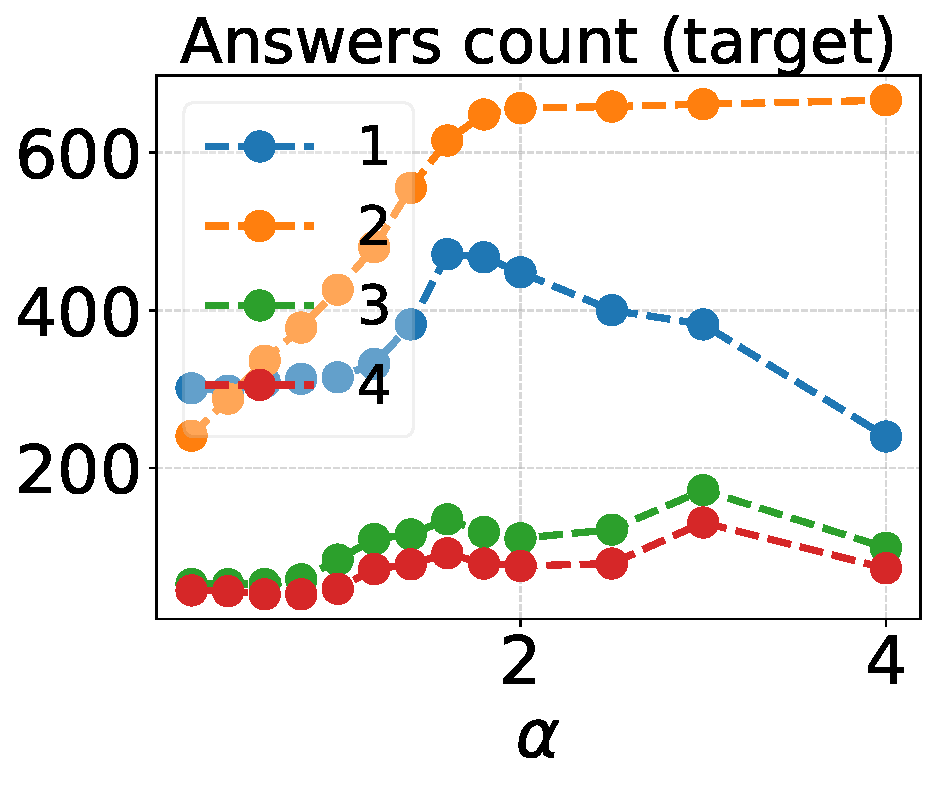
\includegraphics[width=\linewidth]{Figures/model_steering/ablate_alpha/answers_type/model_steering_shift_of_means_ablate_alpha_llava_type_number_Answers_count_.pdf}
        \end{minipage}%
        \begin{minipage}{0.32\linewidth} %
            \centering
            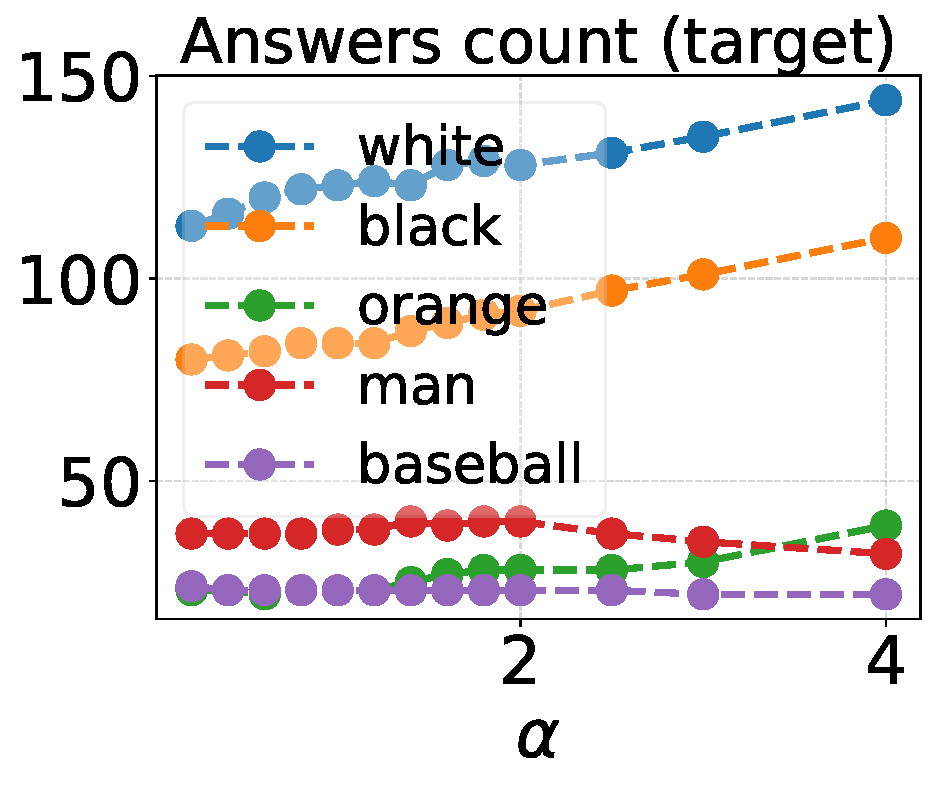
\includegraphics[width=\linewidth]{Figures/model_steering/ablate_alpha/answers_type/model_steering_shift_of_means_ablate_alpha_llava_type_other_Answers_count_.pdf}
        \end{minipage}%

        
    \end{minipage}%

    \caption{\textbf{Ablation study: steering strength ($\alpha$) and changing answer types.} From left to right: steering answers type towards: yes/no, number and other. We report the number of occurrences of some answers in each type. Increasing $\alpha$ pushes the model to generate few answers significantly more than others.}
    \label{fig:model_steering_ablate_alpha_answers_type_words}
\end{figure}





\paragraph{Steering MLLMs answer types.} Similarly, we vary $\alpha$ while changing the model answers to be from a particular type. Note that, here the steering should not be targeted as the goal is to change all answers (\emph{i.e.}, the steering vector is computed to steer the answers from random samples towards samples from a the target type). \Cref{fig:model_steering_ablate_alpha_answers_type} shows that increasing $\alpha$ pushes the model to generate more answers from the target type. However, \Cref{fig:model_steering_ablate_alpha_answers_type_words} shows that increasing the $\alpha$ significantly makes the model generate only few answers from the target type, which makes the generation less diverse.



\begin{figure}[t]
    \centering
    \begin{minipage}{1\linewidth}
    
        \begin{minipage}{0.32\linewidth} %
            \centering
            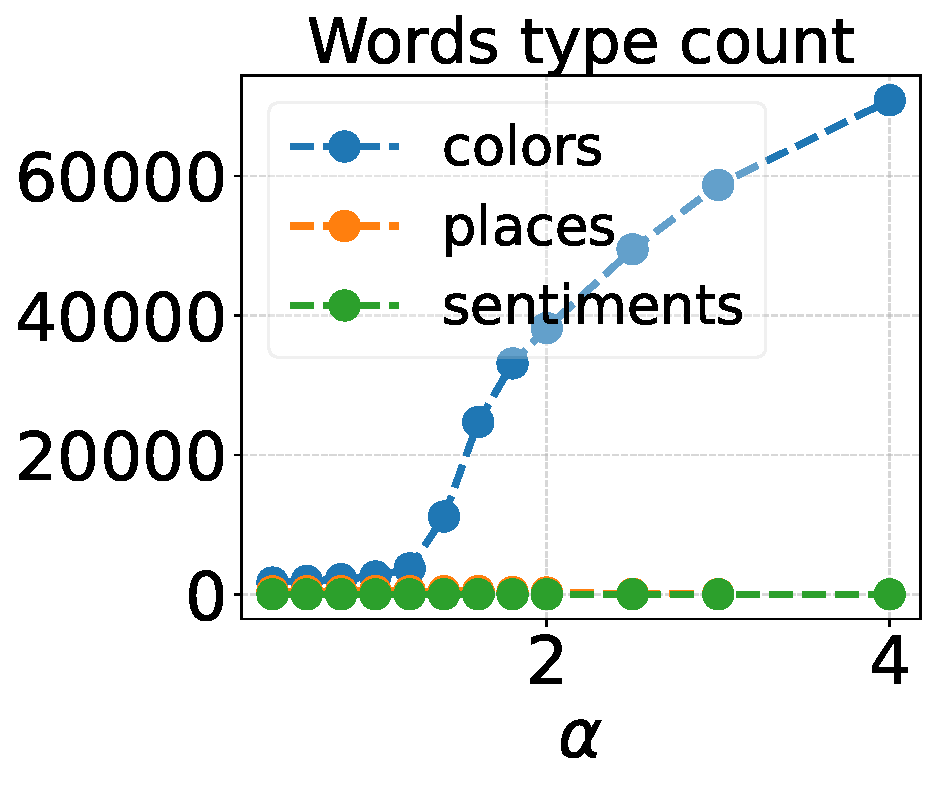
\includegraphics[width=\linewidth]{Figures/model_steering/ablate_alpha/captions_type/model_steering_shift_of_means_ablate_alpha_llava_coco_19_class_onlytoi_colors_Words_type_count.pdf}
        \end{minipage}%
        \begin{minipage}{0.32\linewidth} %
            \centering
            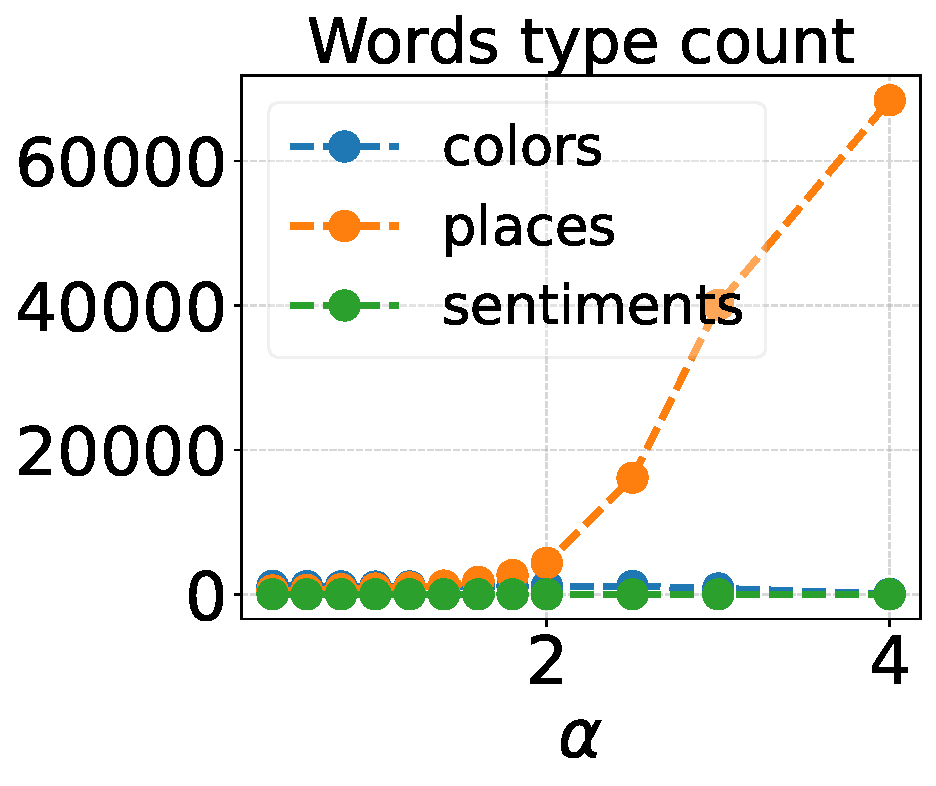
\includegraphics[width=\linewidth]{Figures/model_steering/ablate_alpha/captions_type/model_steering_shift_of_means_ablate_alpha_llava_coco_19_class_onlytoi_places_Words_type_count.pdf}
        \end{minipage}%
        \begin{minipage}{0.32\linewidth} %
            \centering
            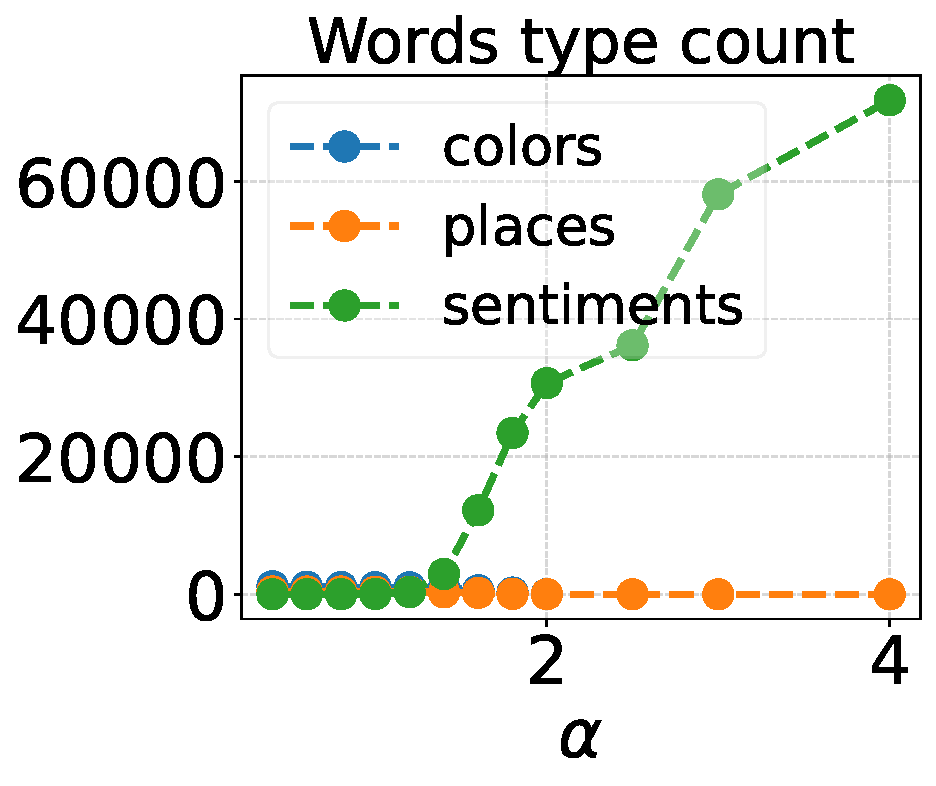
\includegraphics[width=\linewidth]{Figures/model_steering/ablate_alpha/captions_type/model_steering_shift_of_means_ablate_alpha_llava_coco_19_class_onlytoi_positive_sentiments_Words_type_count.pdf}
        \end{minipage}%

    
    \end{minipage}%


    \caption{\textbf{Ablation study: steering strength ($\alpha$) and changing caption styles.} From left to right: steering captions style to include more: colors, places and sentiments. We report the number words belonging to each type. Increasing $\alpha$ pushes the model to generate words related to the traget style.}
    \label{fig:model_steering_ablate_alpha_captions_type_count}
\end{figure}


\begin{figure}[t]
    \centering
    \begin{minipage}{1\linewidth}
    
        \begin{minipage}{0.32\linewidth} %
            \centering
            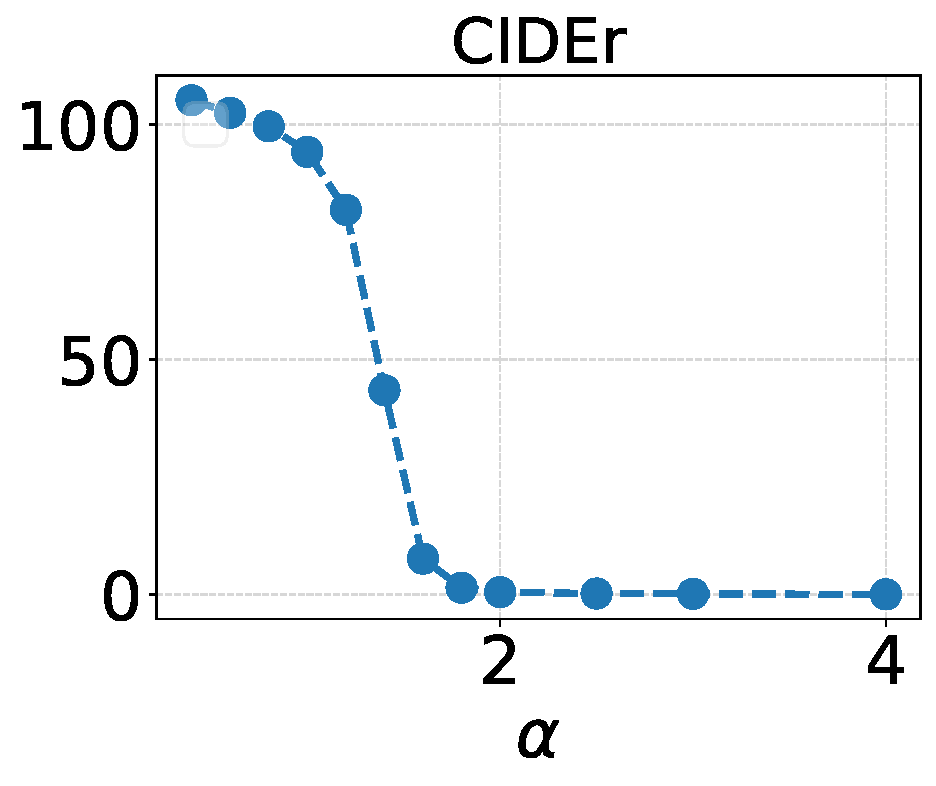
\includegraphics[width=\linewidth]{Figures/model_steering/ablate_alpha/captions_type/model_steering_shift_of_means_ablate_alpha_llava_coco_19_class_onlytoi_colors_CIDEr.pdf}
        \end{minipage}%
        \begin{minipage}{0.32\linewidth} %
            \centering
            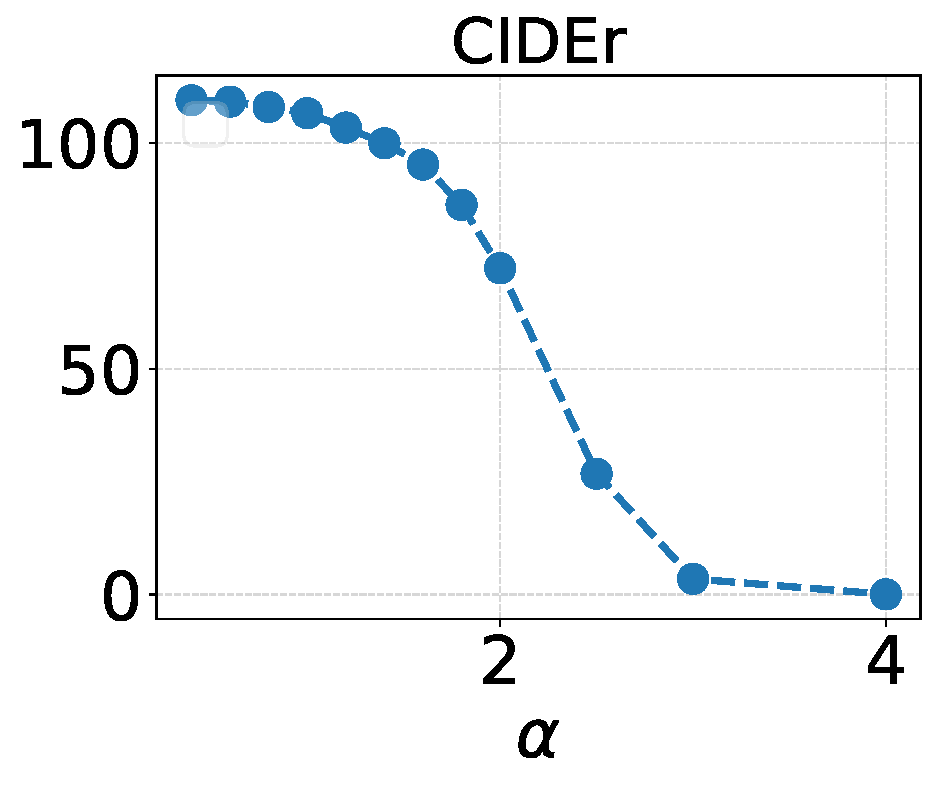
\includegraphics[width=\linewidth]{Figures/model_steering/ablate_alpha/captions_type/model_steering_shift_of_means_ablate_alpha_llava_coco_19_class_onlytoi_places_CIDEr.pdf}
        \end{minipage}%
        \begin{minipage}{0.32\linewidth} %
            \centering
            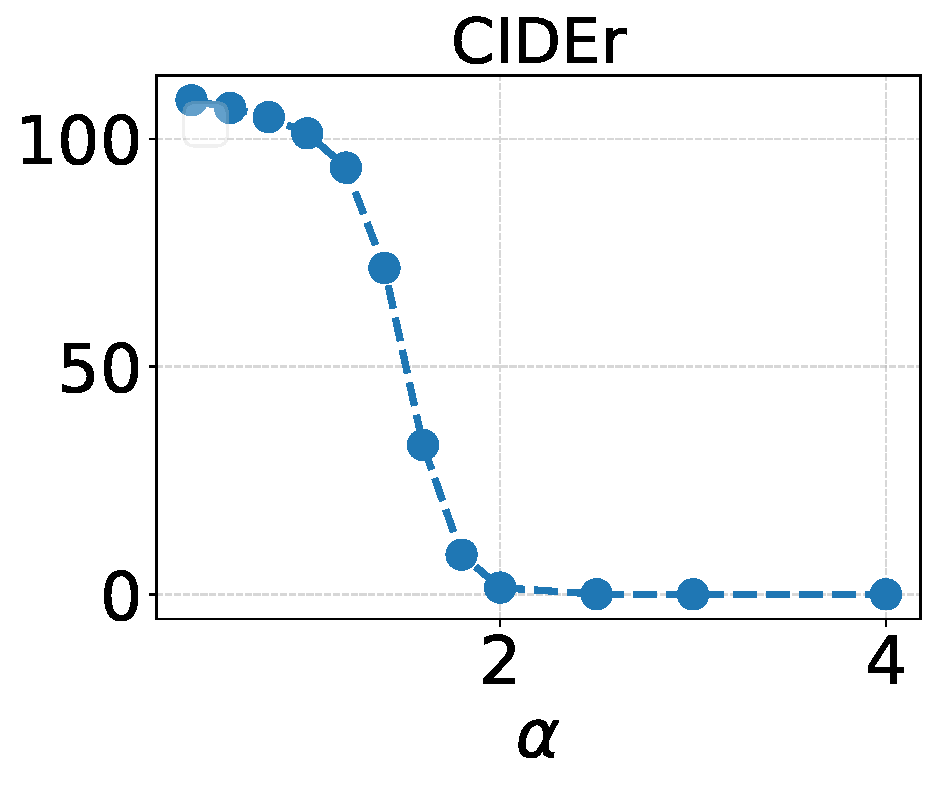
\includegraphics[width=\linewidth]{Figures/model_steering/ablate_alpha/captions_type/model_steering_shift_of_means_ablate_alpha_llava_coco_19_class_onlytoi_positive_sentiments_CIDEr.pdf}
        \end{minipage}%

    
    \end{minipage}%


    \caption{\textbf{Ablation study: steering strength ($\alpha$) and changing caption styles.} From left to right: steering captions style to include more: colors, places and sentiments. We report the CIDEr score. Despite having more captions from the target style, significantly increasing $\alpha$ leads to significant degradation in captioning quality. Note that the CIDEr is expected to decrease as changing the style deviates the captions more from the ground truth. However, we see huge drop when $\alpha$ goes beyond 1.}
    \label{fig:model_steering_ablate_alpha_captions_type_cider}
\end{figure}



\begin{figure*}[t]
    \centering
    \begin{minipage}{0.8\linewidth}
    \centering
        \begin{minipage}{0.24\linewidth}
            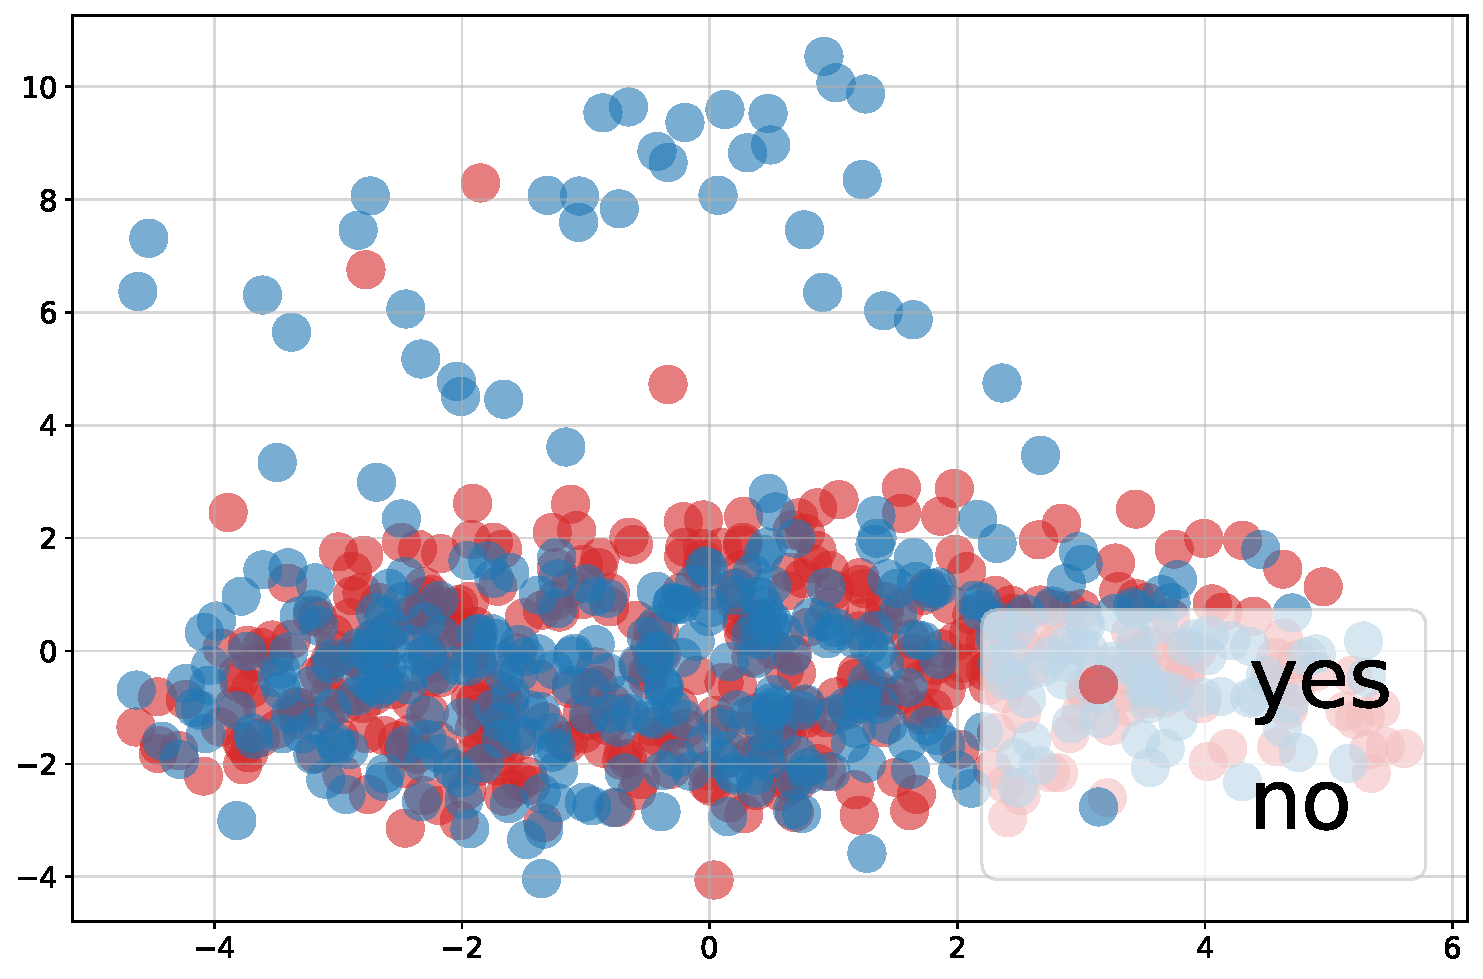
\includegraphics[width=1.0\textwidth]{Figures/model_steering/pca/pca_shift_of_means_llava_11_yes_to_no.pdf}
        \end{minipage}%
        \begin{minipage}{0.24\linewidth}
            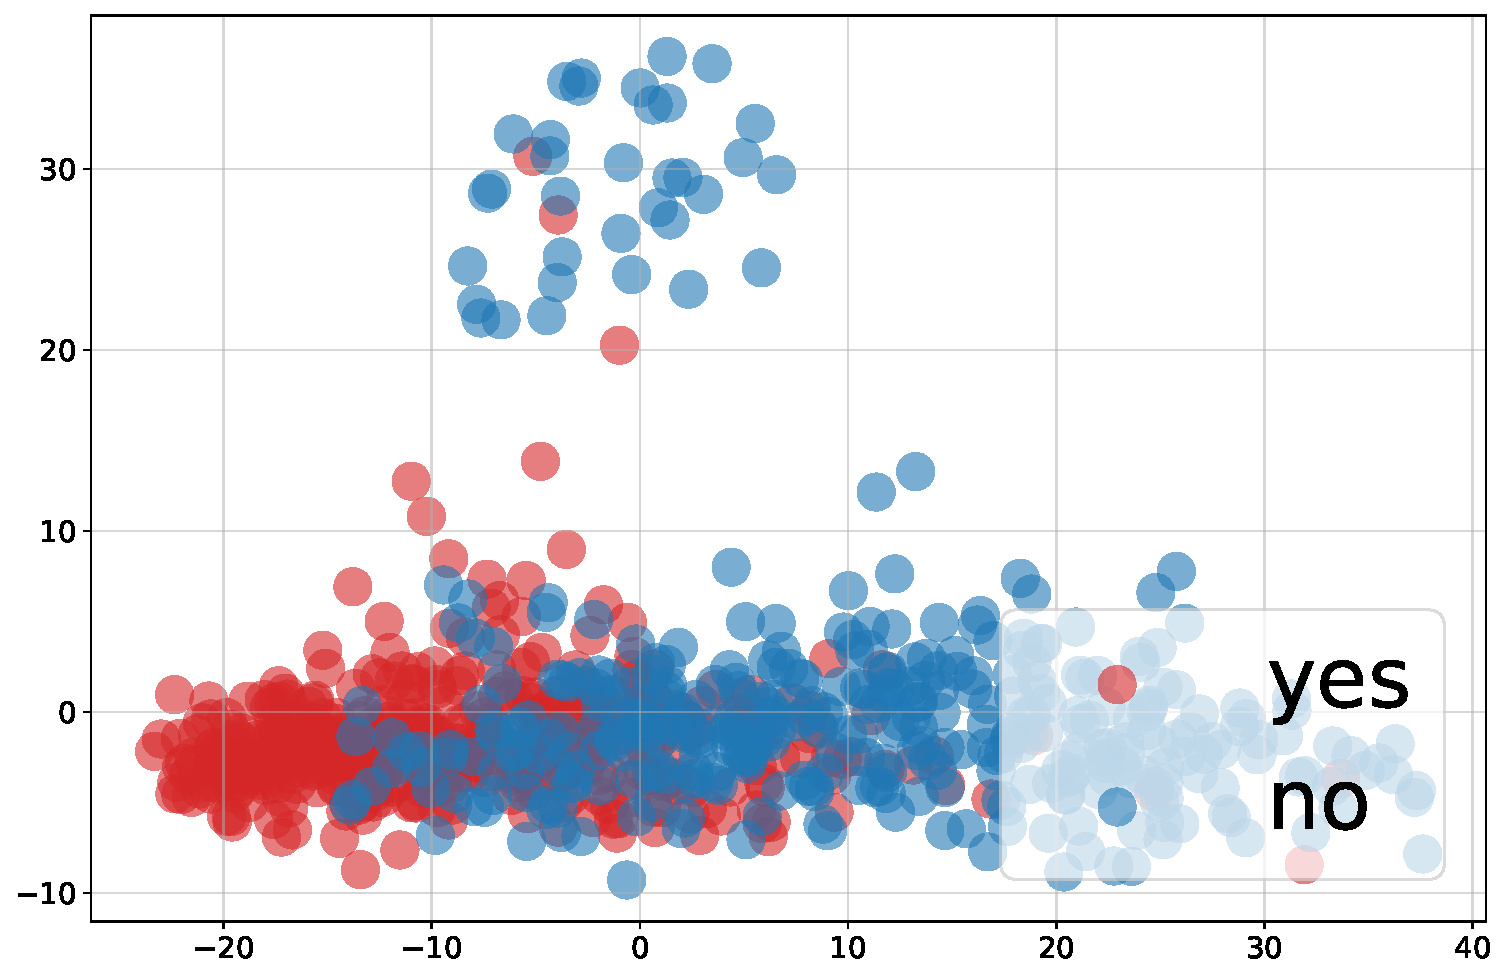
\includegraphics[width=1.0\textwidth]{Figures/model_steering/pca/pca_shift_of_means_llava_19_yes_to_no.pdf}
        \end{minipage}%
        \begin{minipage}{0.24\linewidth}
            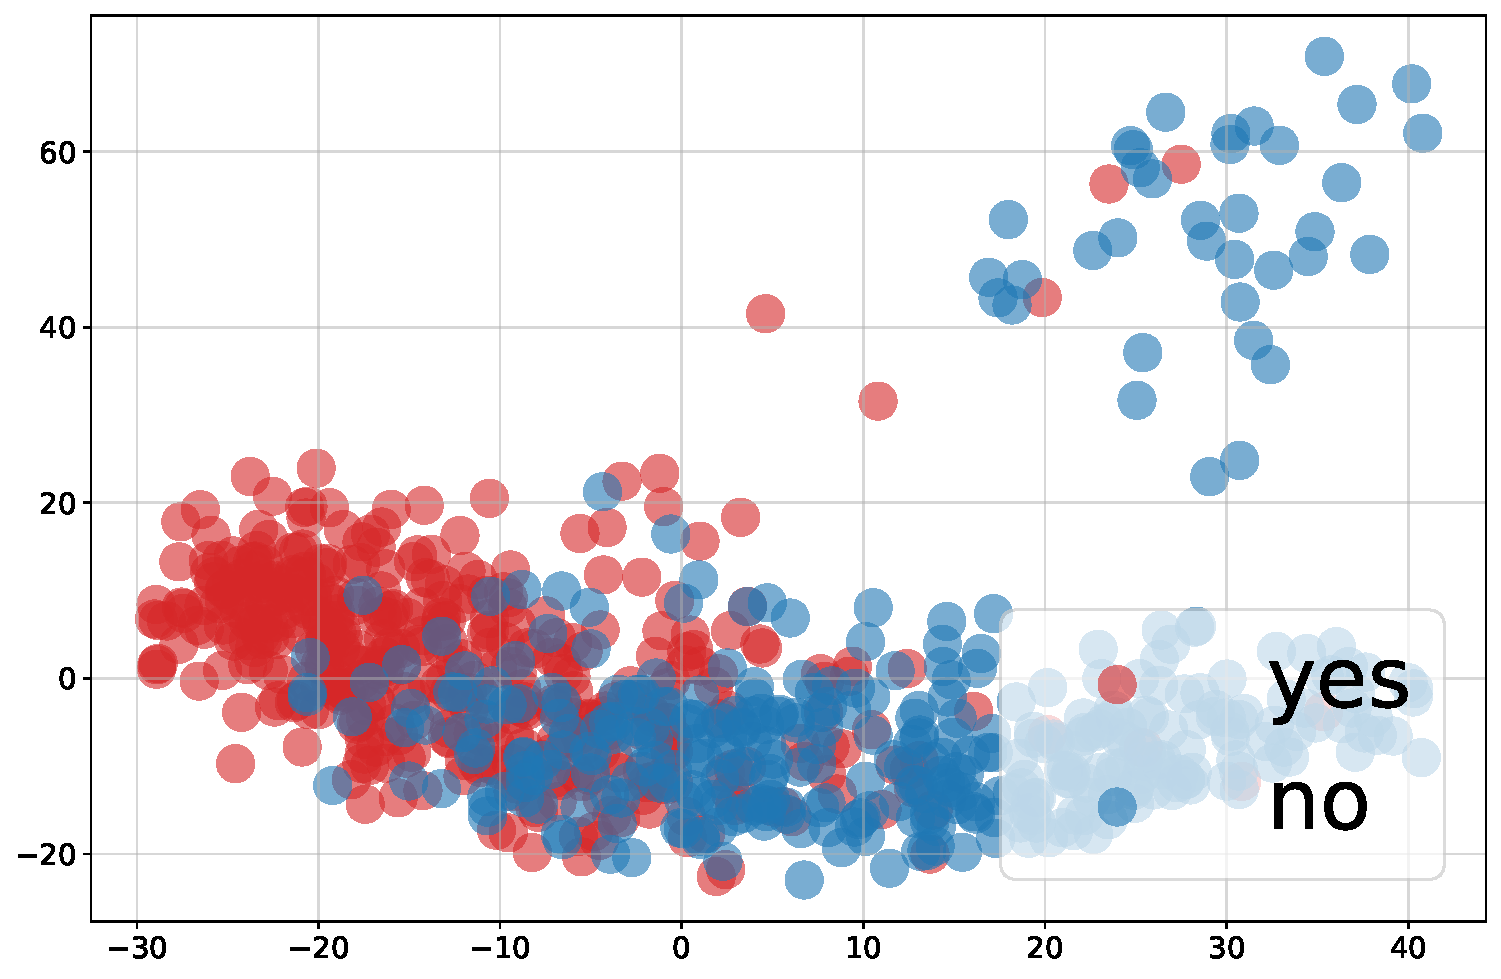
\includegraphics[width=1.0\textwidth]{Figures/model_steering/pca/pca_shift_of_means_llava_25_yes_to_no.pdf}
        \end{minipage}%
        \begin{minipage}{0.24\linewidth}
            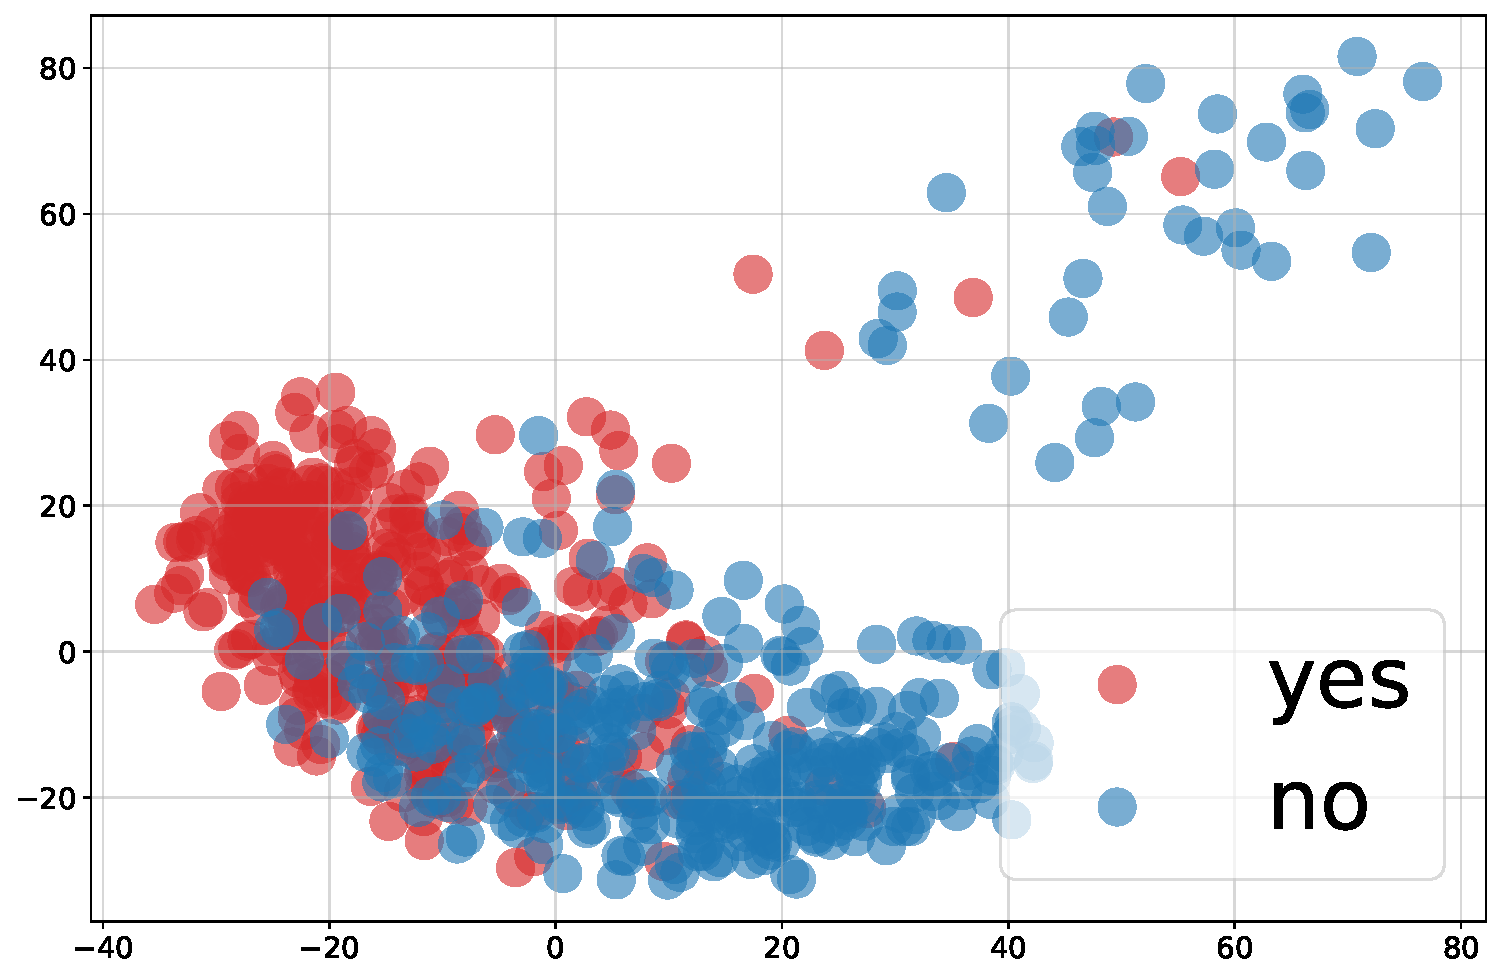
\includegraphics[width=1.0\textwidth]{Figures/model_steering/pca/pca_shift_of_means_llava_29_yes_to_no.pdf}
        \end{minipage}%
    
        \begin{minipage}{0.24\linewidth}
            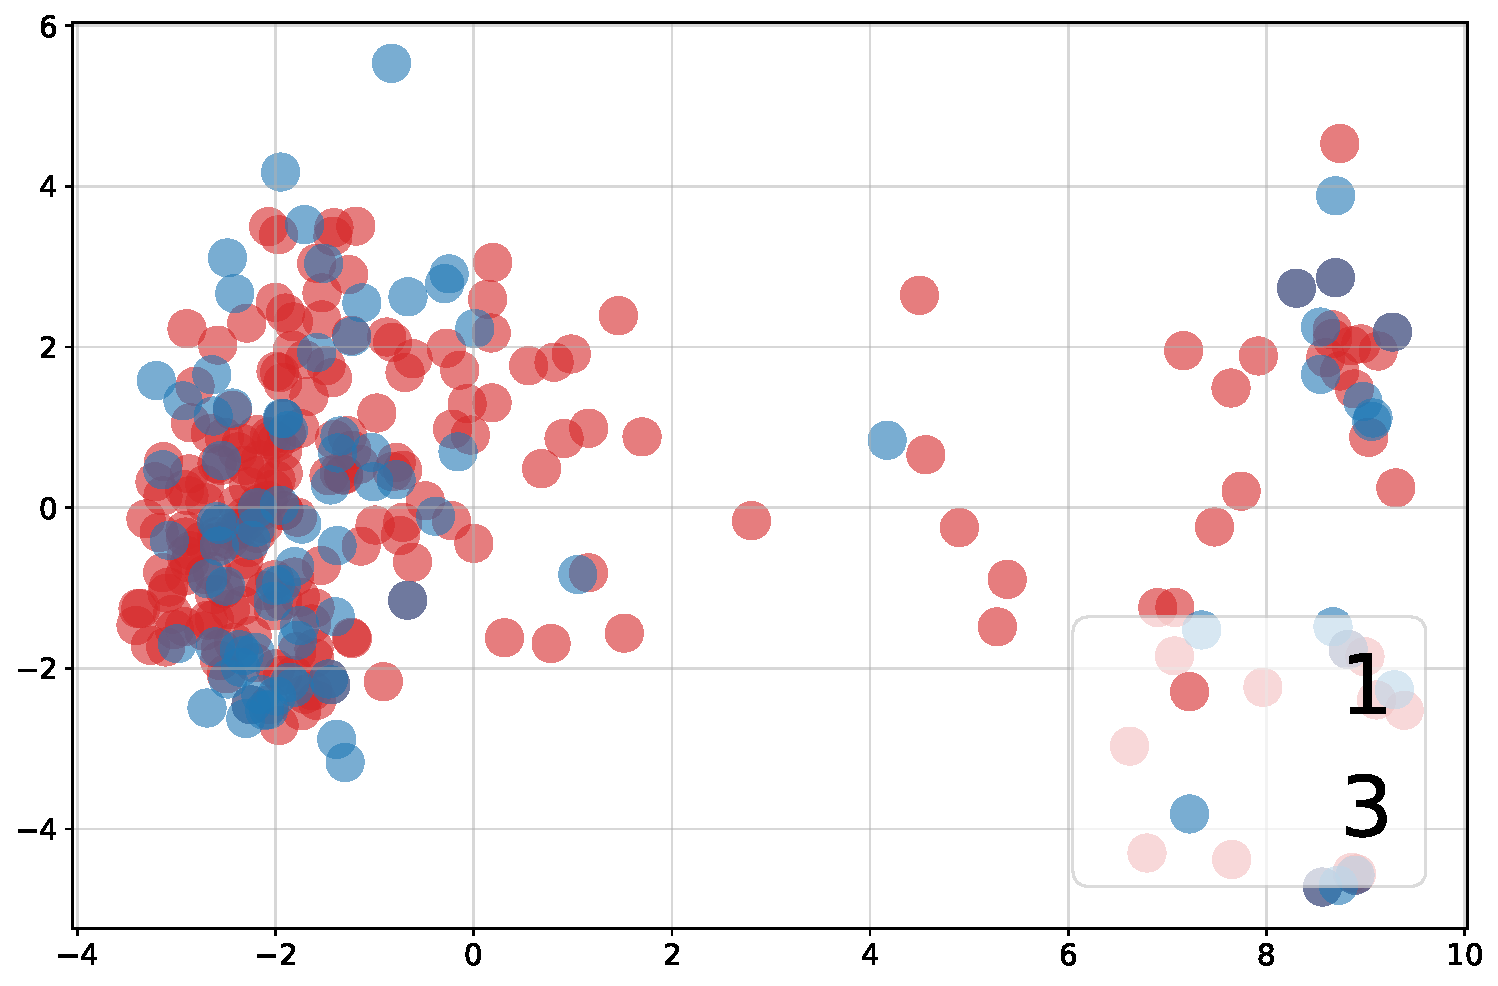
\includegraphics[width=1.0\textwidth]{Figures/model_steering/pca/pca_shift_of_means_llava_11_1_to_3.pdf}
        \end{minipage}%
        \begin{minipage}{0.24\linewidth}
            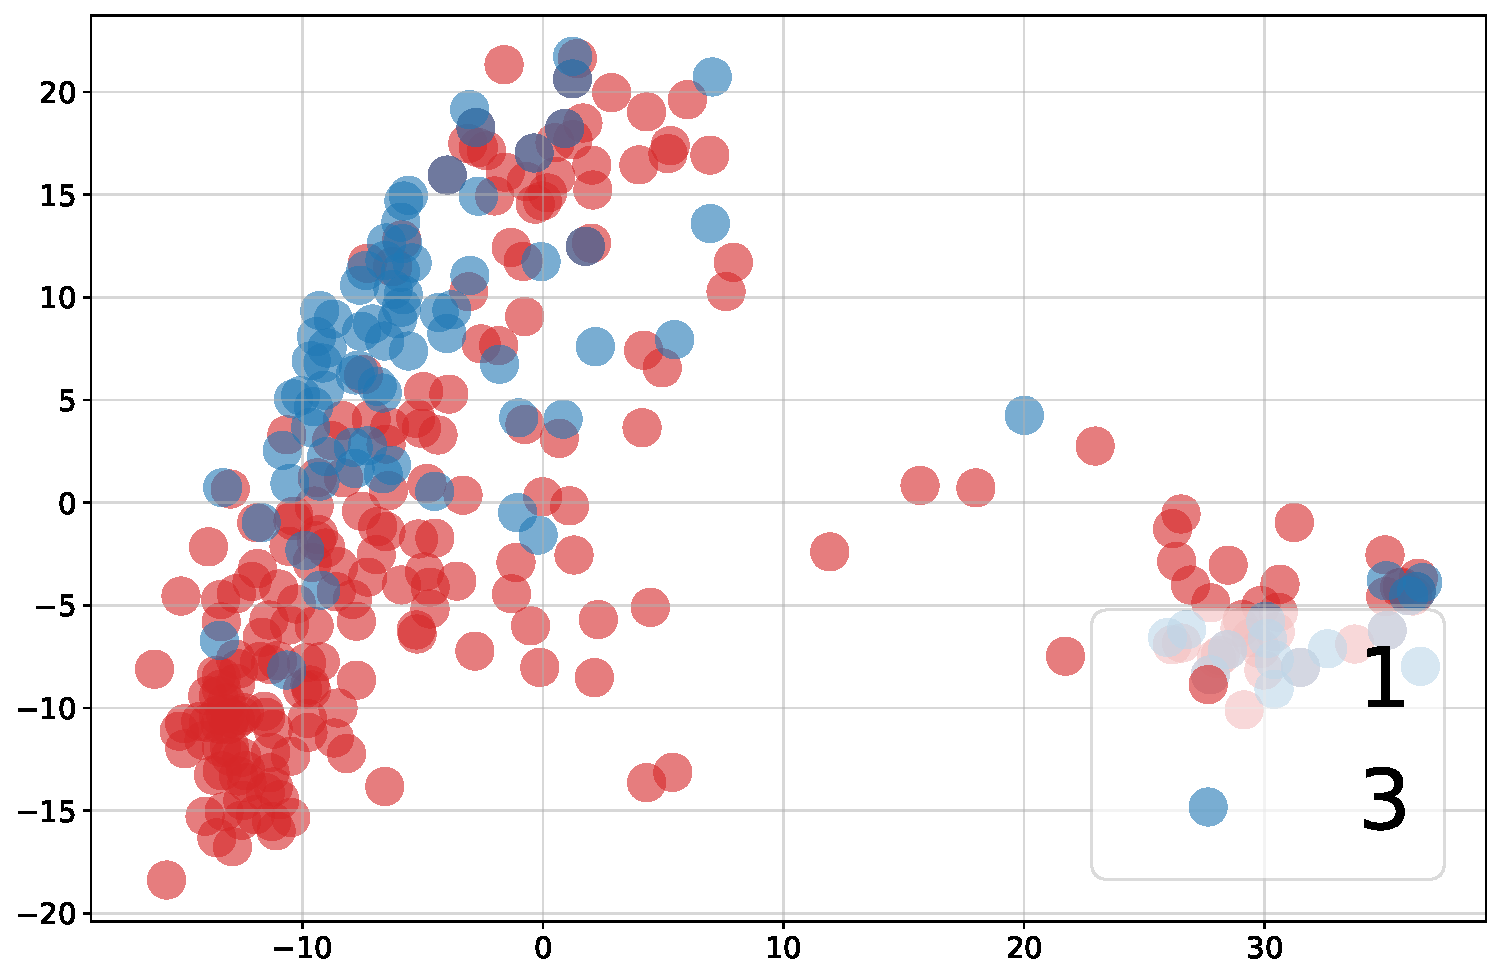
\includegraphics[width=1.0\textwidth]{Figures/model_steering/pca/pca_shift_of_means_llava_19_1_to_3.pdf}
        \end{minipage}%
        \begin{minipage}{0.24\linewidth}
            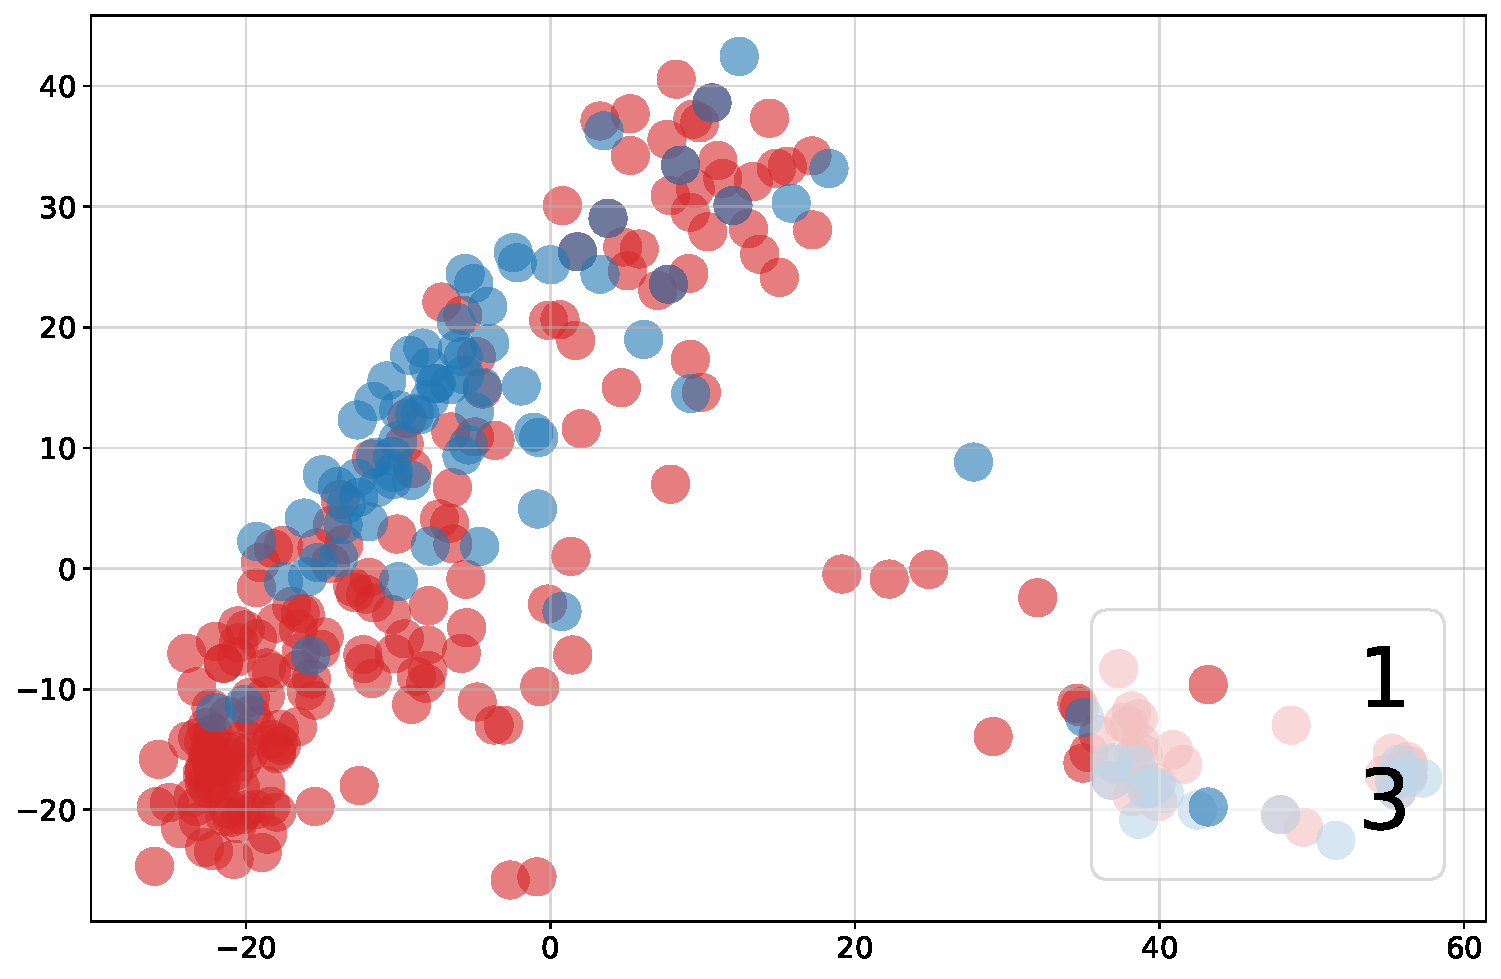
\includegraphics[width=1.0\textwidth]{Figures/model_steering/pca/pca_shift_of_means_llava_25_1_to_3.pdf}
        \end{minipage}%
        \begin{minipage}{0.24\linewidth}
            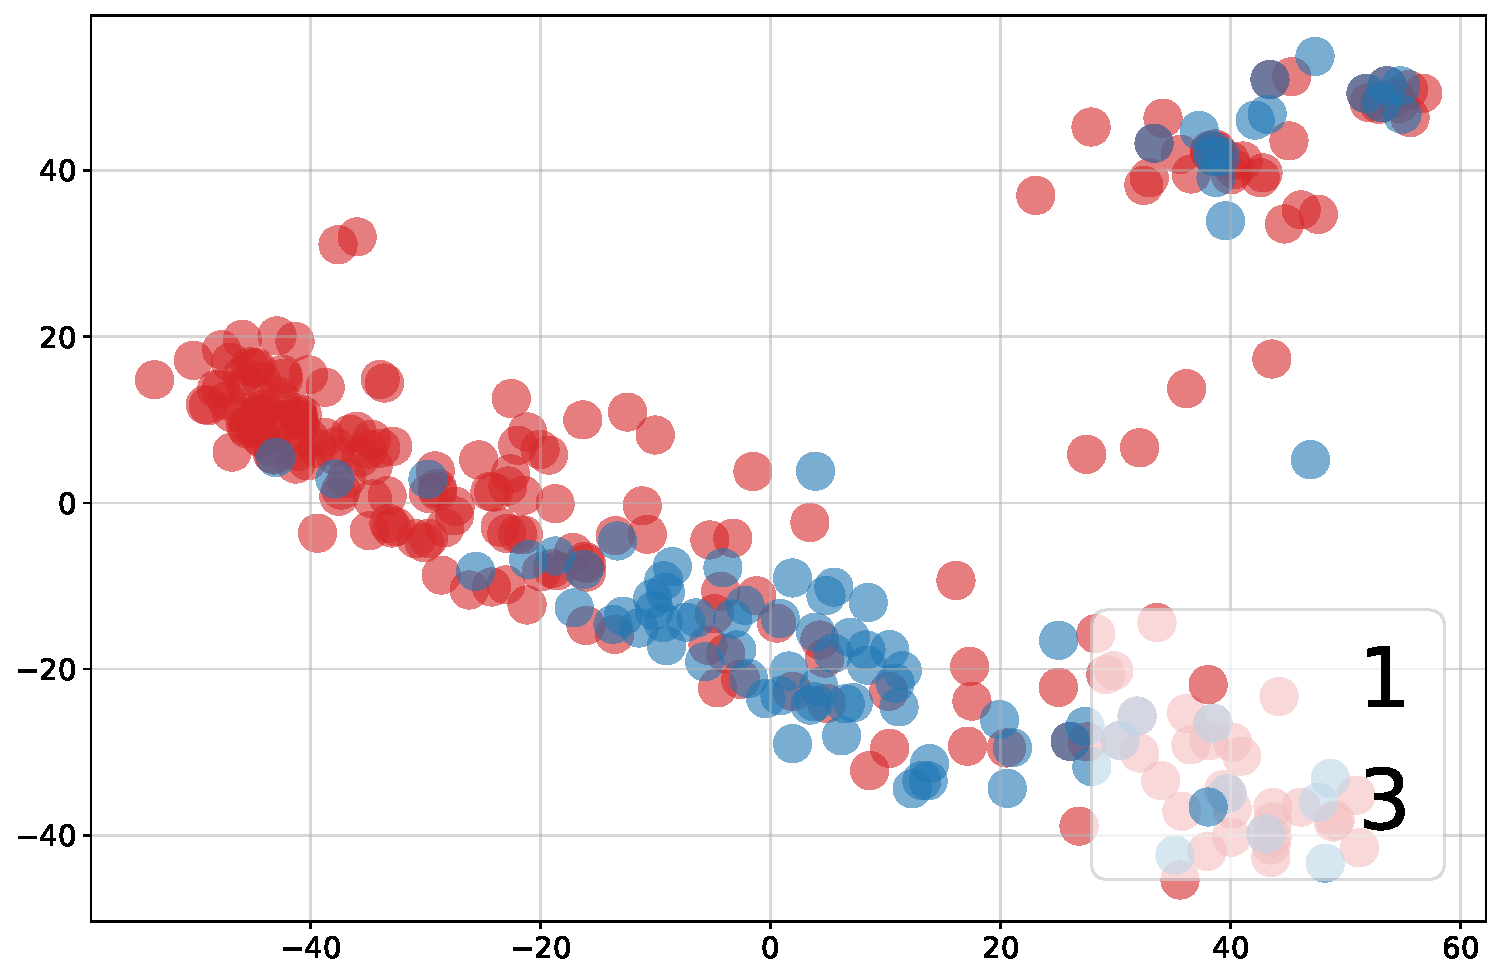
\includegraphics[width=1.0\textwidth]{Figures/model_steering/pca/pca_shift_of_means_llava_29_1_to_3.pdf}
        \end{minipage}%

    
        \begin{minipage}{0.24\linewidth}
            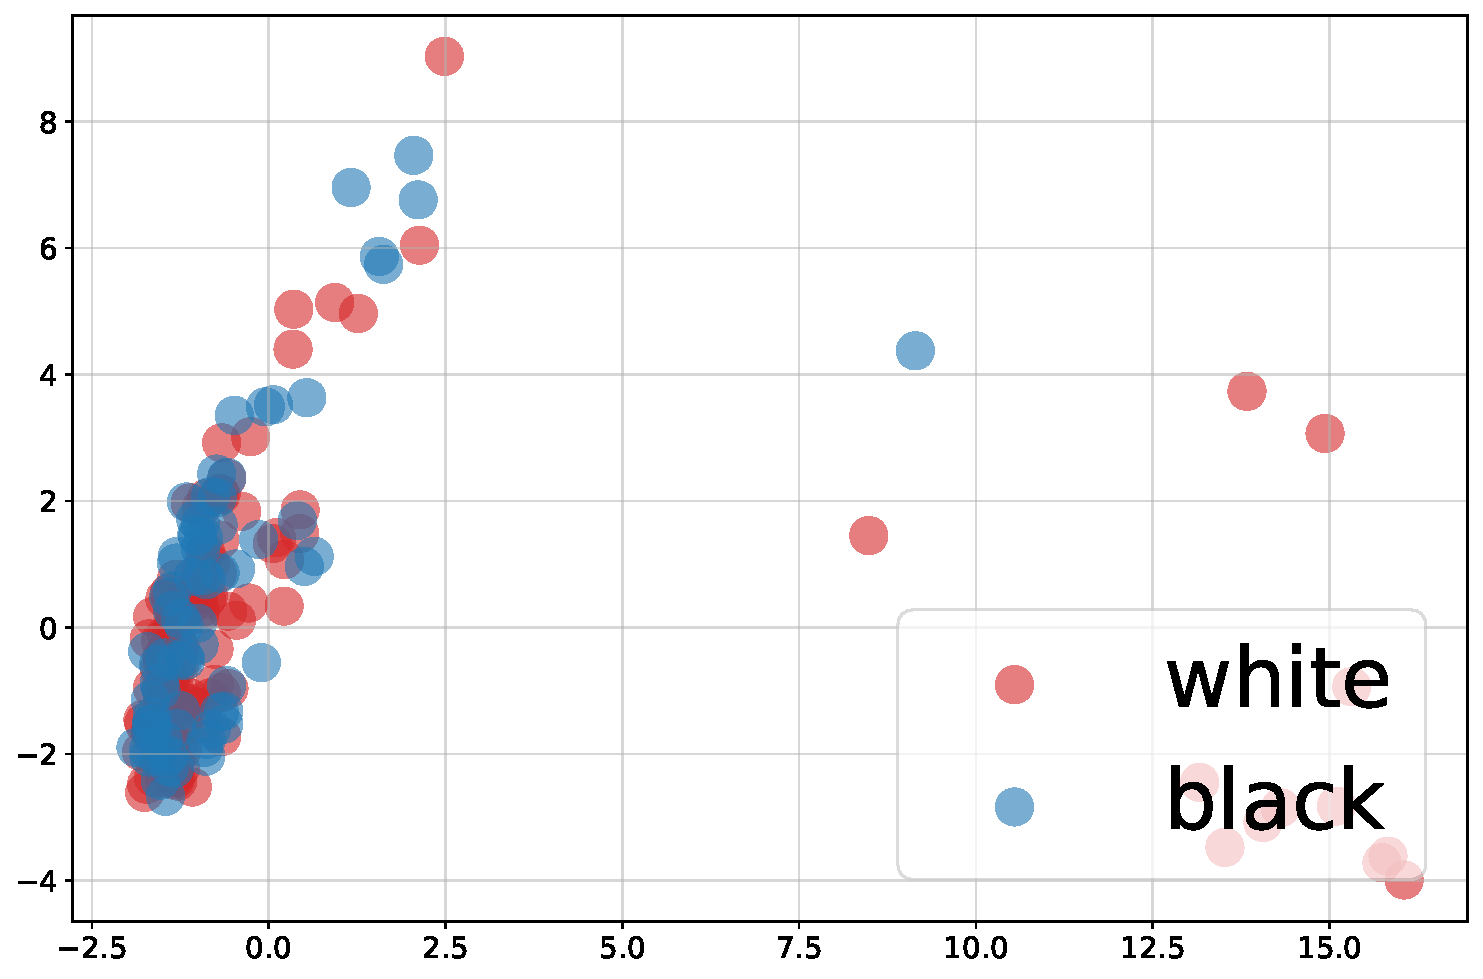
\includegraphics[width=1.0\textwidth]{Figures/model_steering/pca/pca_shift_of_means_llava_11_white_to_black.pdf}
            \caption*{\small{$l=11$}}
        \end{minipage}%
        \begin{minipage}{0.24\linewidth}
            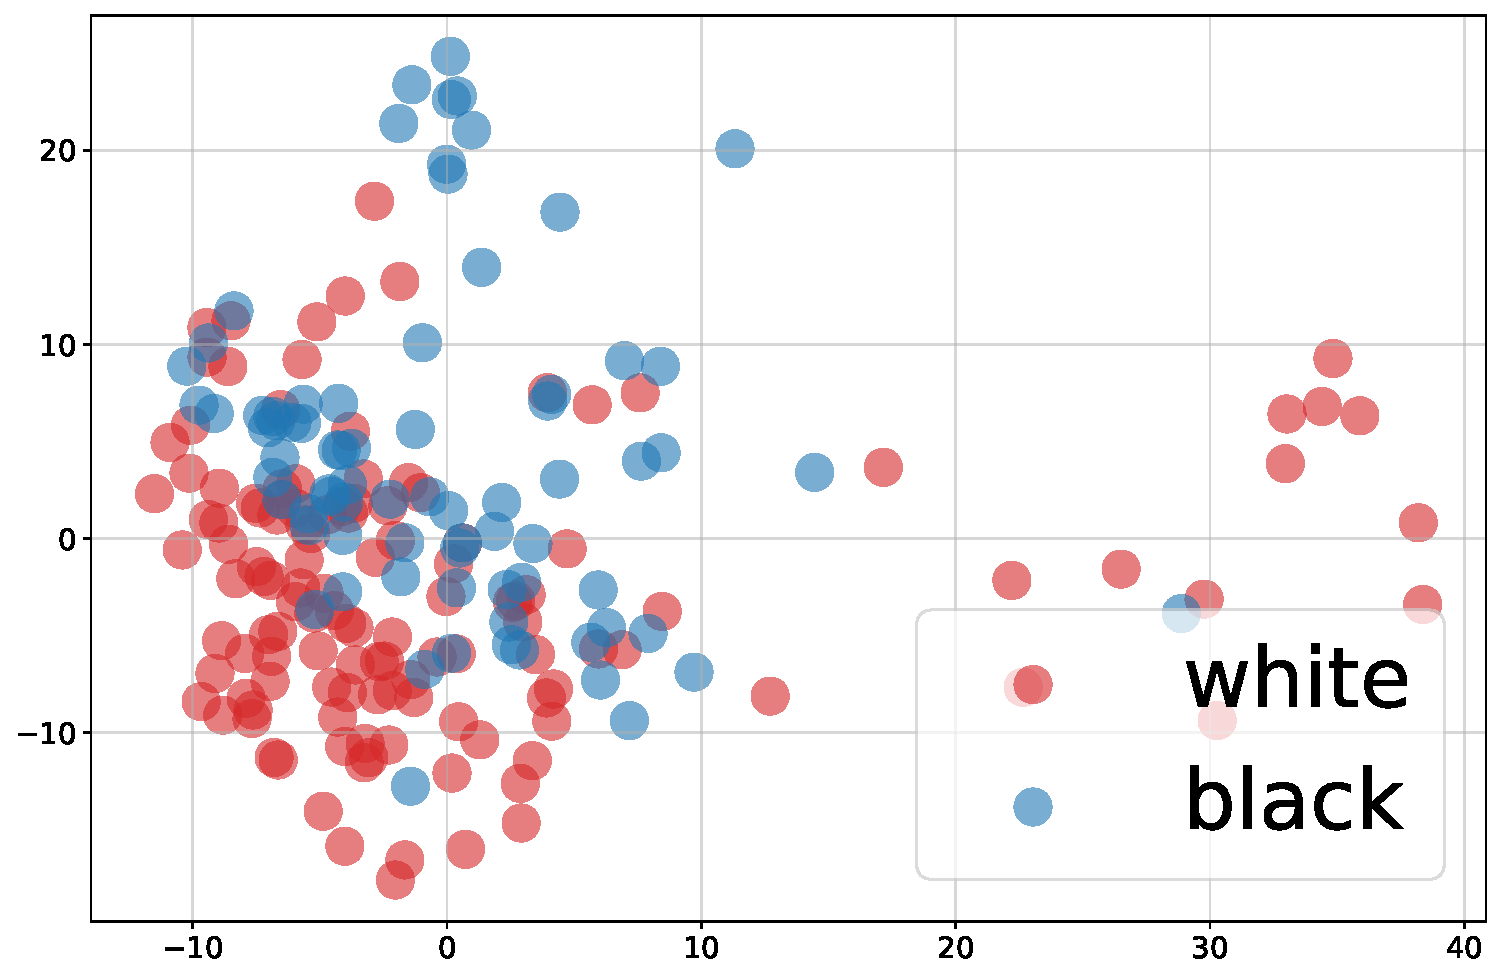
\includegraphics[width=1.0\textwidth]{Figures/model_steering/pca/pca_shift_of_means_llava_19_white_to_black.pdf}
            \caption*{\small{$l=19$}}
        \end{minipage}%
        \begin{minipage}{0.24\linewidth}
            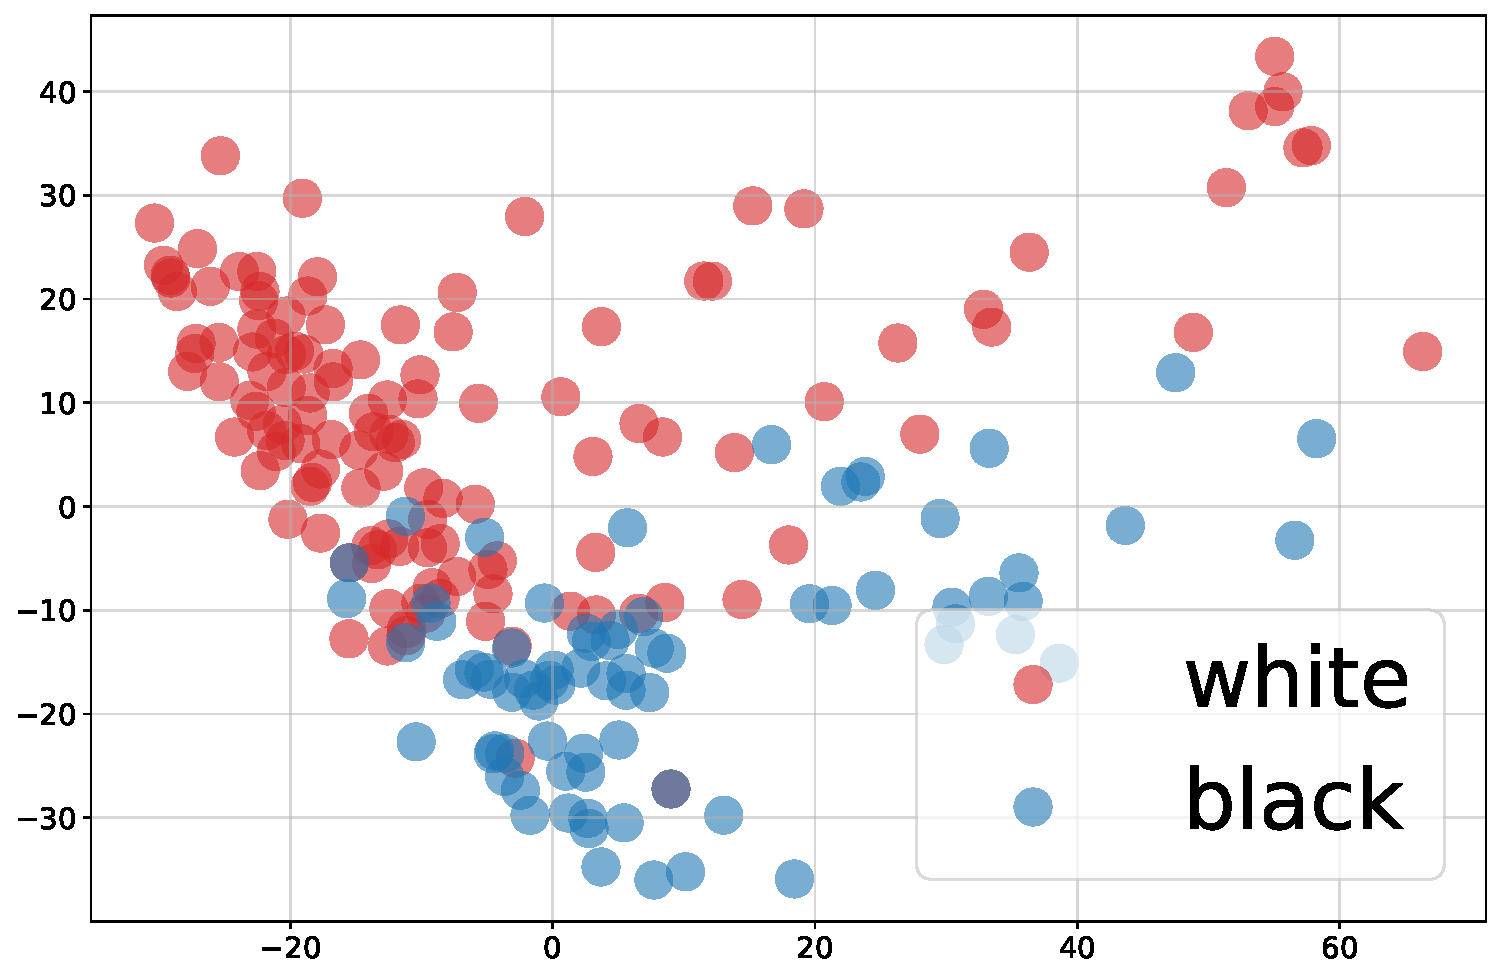
\includegraphics[width=1.0\textwidth]{Figures/model_steering/pca/pca_shift_of_means_llava_25_white_to_black.pdf}
            \caption*{\small{$l=25$}}
        \end{minipage}%
        \begin{minipage}{0.24\linewidth}
            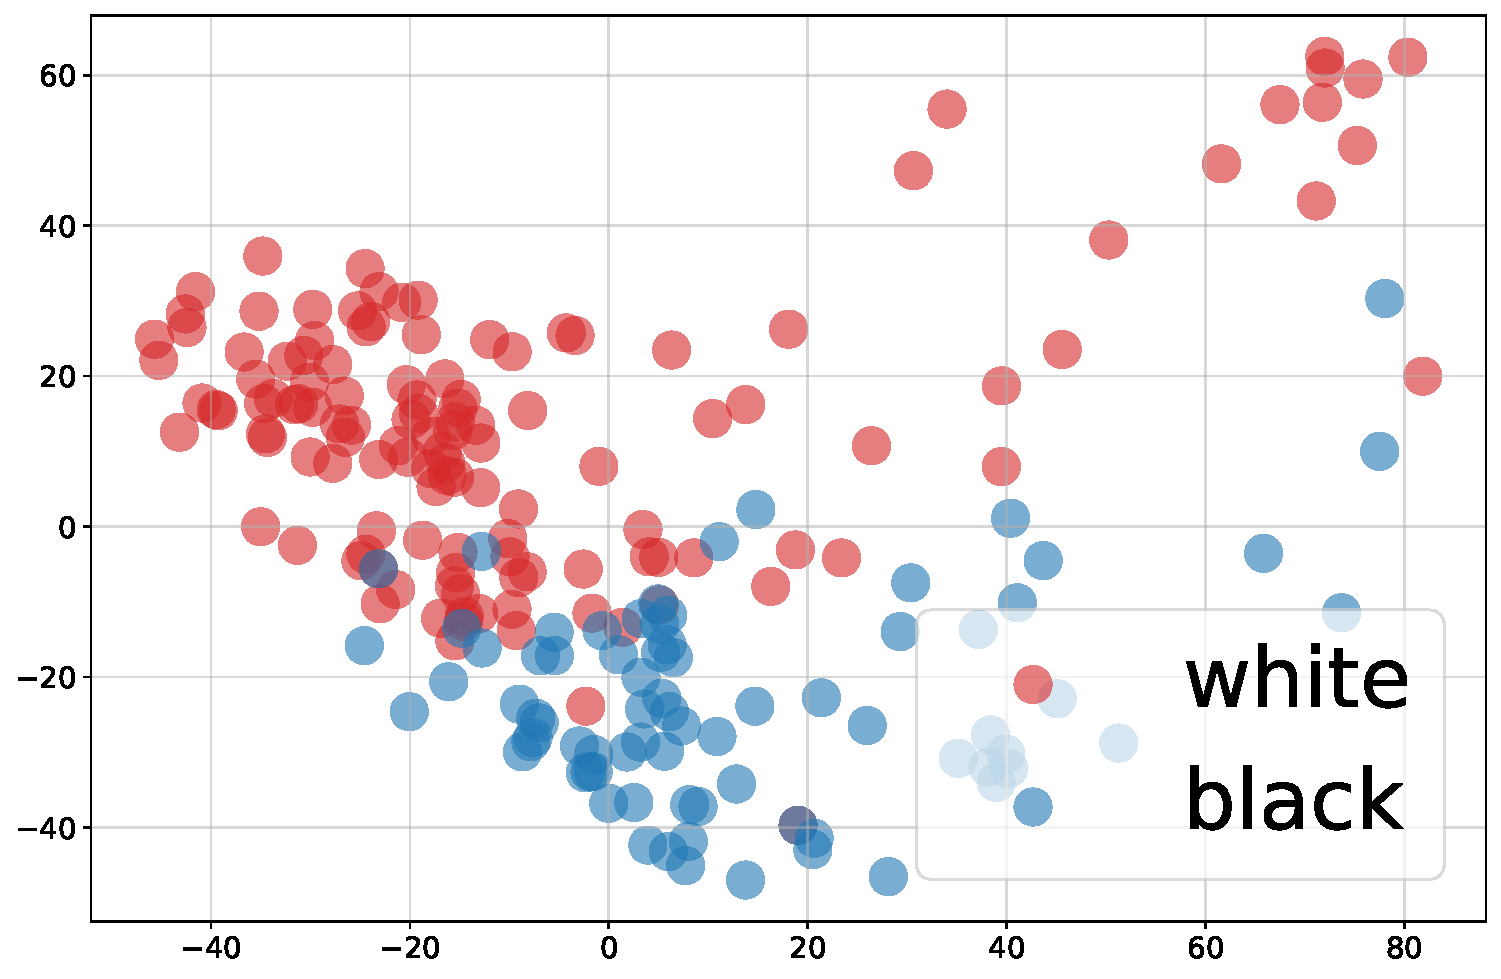
\includegraphics[width=1.0\textwidth]{Figures/model_steering/pca/pca_shift_of_means_llava_29_white_to_black.pdf}
            \caption*{\small{$l=29$}}
        \end{minipage}%

\end{minipage}%
\caption{\textbf{Linear separability of concepts features in MLLMs.} We visualize the features related to the concepts \textcolor{BrickRed}{"yes"}/\textcolor{NavyBlue}{"no"}, \textcolor{BrickRed}{"1"}/\textcolor{NavyBlue}{"3"} and \textcolor{BrickRed}{"white"}/\textcolor{NavyBlue}{"black"} after PCA projections across MLLMs layers.}
\label{fig:app_model_steering_qual_pca_concepts_samples}
\end{figure*}



\begin{figure}[t]
    \centering
    \begin{minipage}{\linewidth}
    \centering
        \begin{minipage}{\linewidth}
            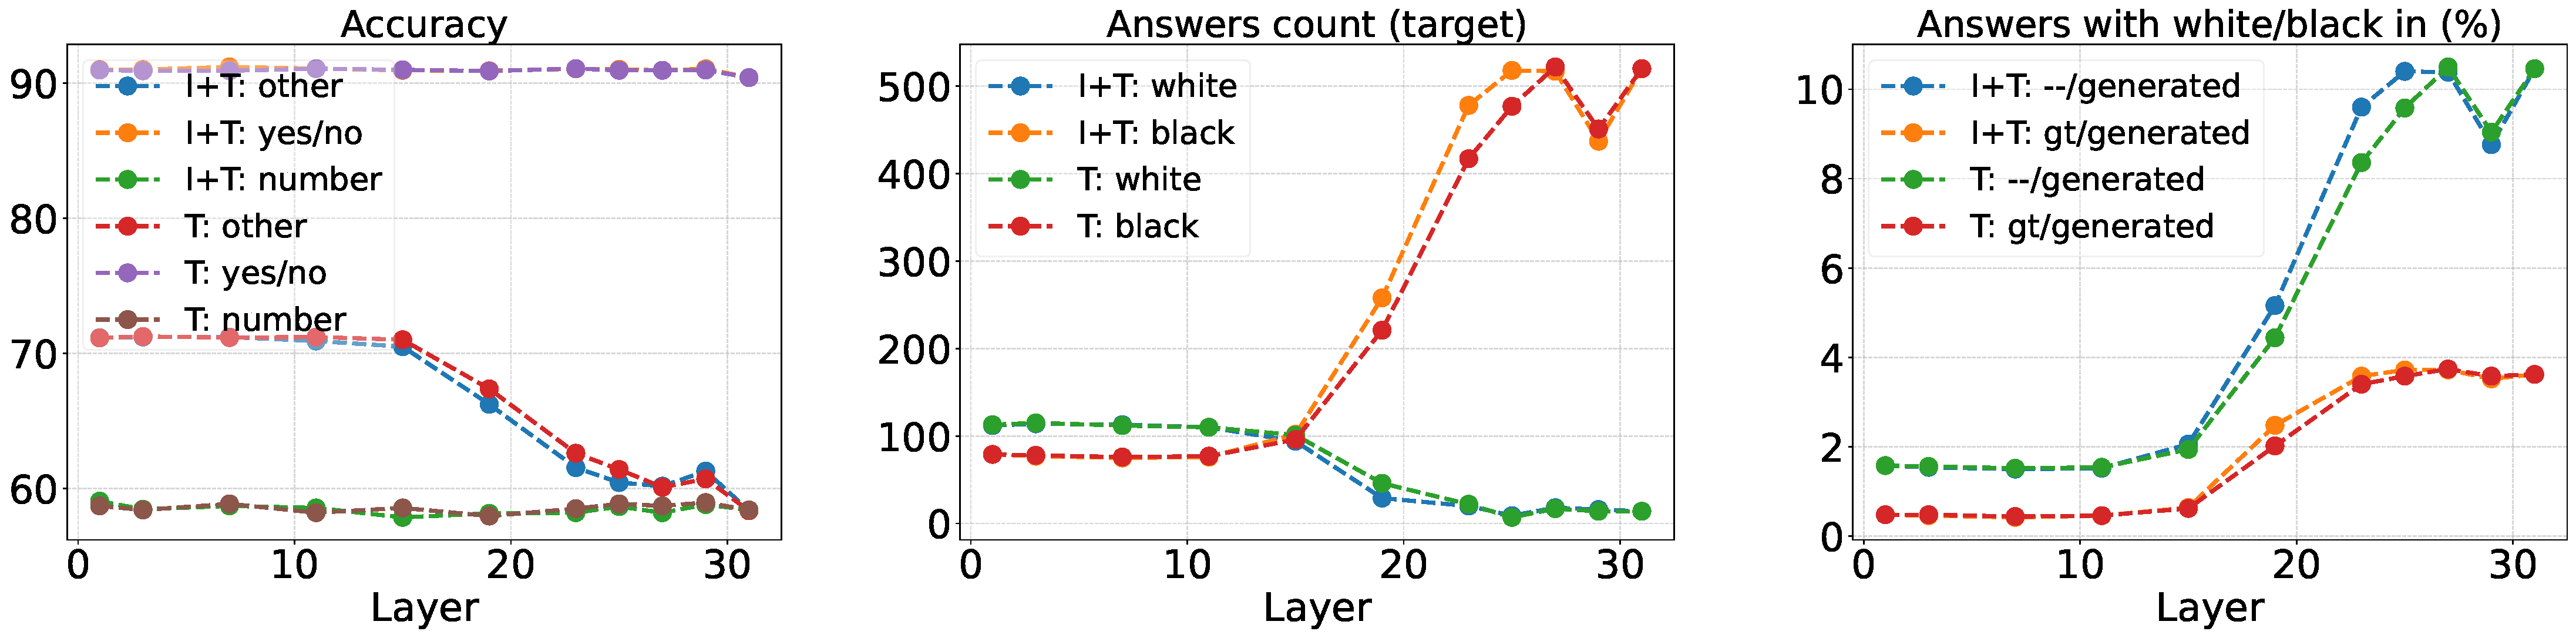
\includegraphics[width=1.0\textwidth]{Figures/model_steering/ablate_steering_tokens/model_steering_shift_of_means_ablate_steering_tokens_white_to_black_all_txt_Accuracy_Answers_count__Answers_with_white.pdf}
        \end{minipage}%
        
        \begin{minipage}{\linewidth}
            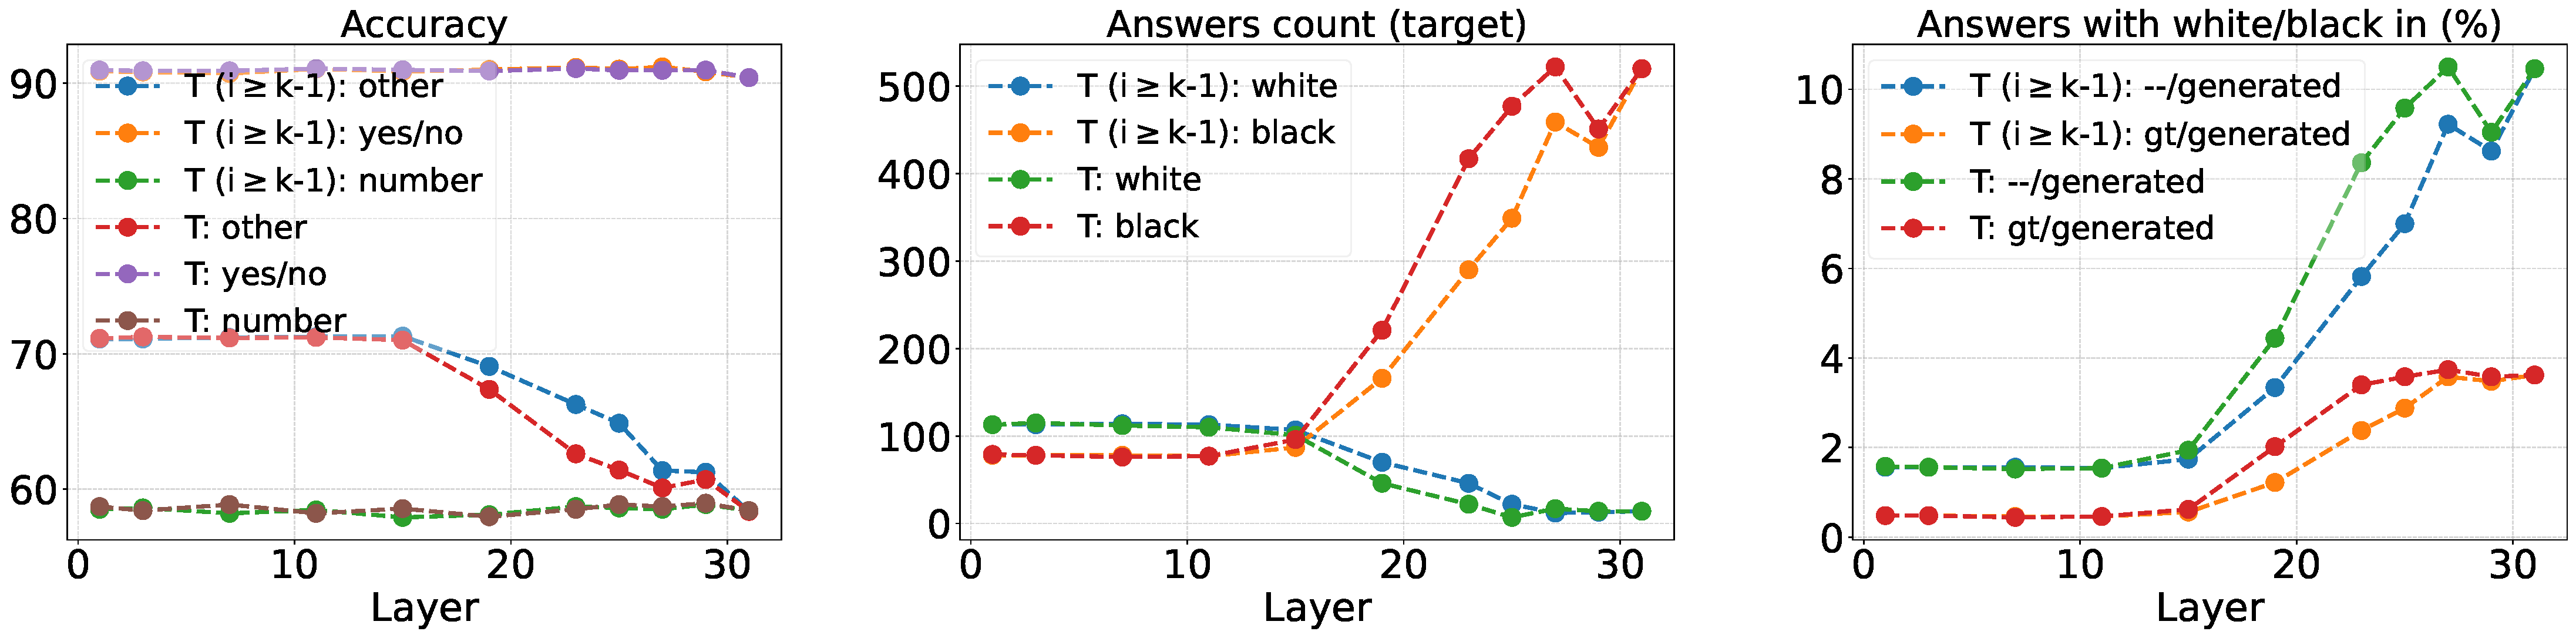
\includegraphics[width=1.0\textwidth]{Figures/model_steering/ablate_steering_tokens/model_steering_shift_of_means_ablate_steering_tokens_white_to_black_last_txt_Accuracy_Answers_count__Answers_with_white.pdf}
        \end{minipage}%
        
        \begin{minipage}{\linewidth}
            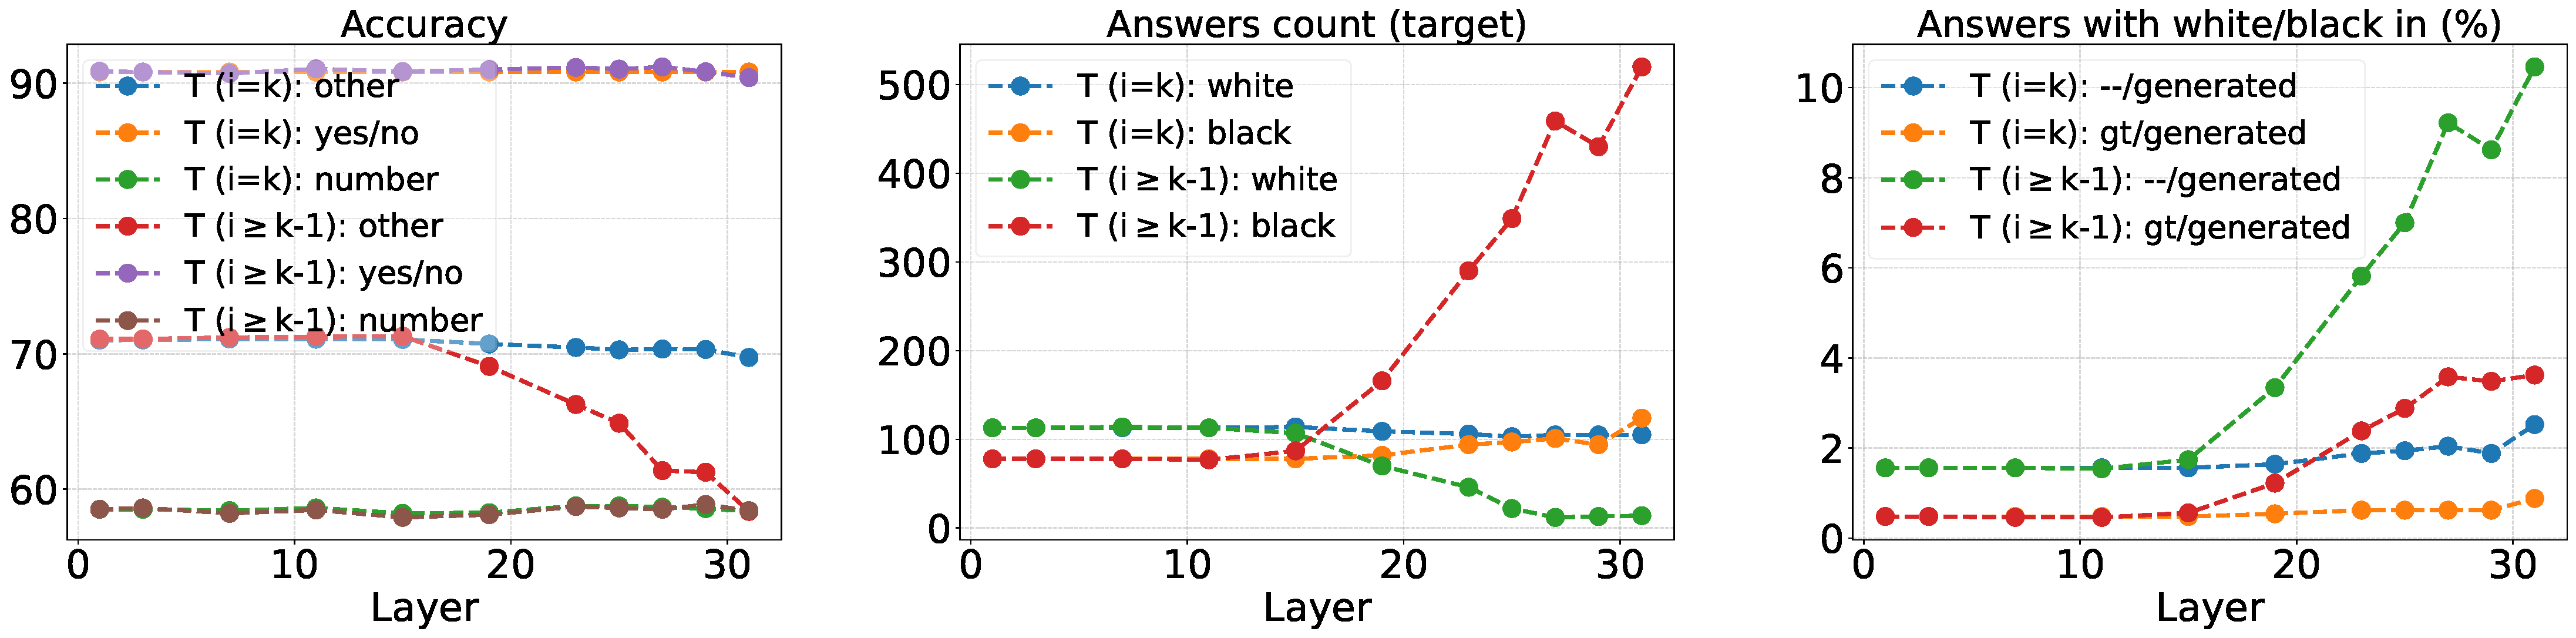
\includegraphics[width=1.0\textwidth]{Figures/model_steering/ablate_steering_tokens/model_steering_shift_of_means_ablate_steering_tokens_white_to_black_gen_last_Accuracy_Answers_count__Answers_with_white.pdf}
        \end{minipage}%
    
    \end{minipage}%
\caption{\textbf{Ablation study: which tokens to apply steering to.} We compare steering: all tokens including image, prompt and generated tokens ($I+T$), only text tokens ($T$, including the prompt and generated ones), only the generated tokens ($T (i=k)$) and last token in the prompt and the generated tokens ($T (i \geq k-1)$). Steering all tokens ($I+T$) has the most steering effect, followed by steering all text tokens ($T$). Steering only the generated tokens has little effect ($T (i=k)$), this can be fixed by steering the token just before ($T (i \geq k-1)$)}
\label{fig:model_steering_ablate_steering_tokens}
\end{figure}


\paragraph{Steering MLLMs image caption styles.} We also study the effect of steering strength on changing the captions styles.\Cref{fig:model_steering_ablate_alpha_captions_type_count} shows, that increasing $\alpha$ leads the model to generate more captions from the target style. However, \Cref{fig:model_steering_ablate_alpha_captions_type_cider} shows that significantly increasing $\alpha$ degrades the quality of the generated captions as seen in the low CIDEr score. Note that, the CIDEr is expected to decrease as changing the caption style leads to deviation from the COCO annotated captions. However, the drastic decrease is due mainly to captions quality. We tried to inspect the output and found that sometimes the model only repeat 1 or 2 words related to the target type. 




\subsubsection{Which tokens to apply steering to?}
\label{sec:app_model_steering_ablation_which_tokens}

In the main paper, we apply the steering vector to all tokens, including the image, instruction and generated ones. Here we study this design choice.\Cref{fig:model_steering_ablate_steering_tokens} illustrates the results. We compare steering: all tokens including image, prompt and generated tokens ($I+T$), only text tokens ($T$, including the prompt and generated ones), only the generated tokens ($T (i=k)$) and last token in the prompt and the generated tokens ($T (i \geq k-1)$). Steering all tokens ($I+T$) has the most steering effect, followed by steering all text tokens ($T$). Steering only the generated tokens has little effect ($T (i=k)$), this can be significantly improved by steering the token just before ($T (i \geq k-1)$).




\subsection{Linear separability of concepts inside MLLMs.}
\label{sec:app_linear_sep}

In this section we investigate why a simple linear operation in the feature space, such as vector addition, is able to steer the model output. To this end, we visualize the PCA projections of the concepts features extracted from different layers inside MLLMs. \Cref{fig:app_model_steering_qual_pca_concepts_samples} shows a clearer separation of concepts when moving to deeper layers, where different concepts can be almost separated linearly. This, tom some extent, validates the linear representation hypothesis for MLLMs, previously studied for LLMs \cite{park2024the,nanda_othello_2023}. In addition, this might explain why applying the steering to deeper layers is more effective than early ones.








\subsection{Qualitative results}
\label{sec:app_model_steering_qual}

We provide additional qualitative results for steering MLLMS answers (\Cref{fig:app_model_steering_qual_change_answers}), answer types (\Cref{fig:model_steering_qual_change_answers_type}) and caption styles
(\Cref{fig:model_steering_qual_change_captions_type})

\newpage

\begin{figure*}[t]
    \centering
    \begin{minipage}{\linewidth}
    \centering
        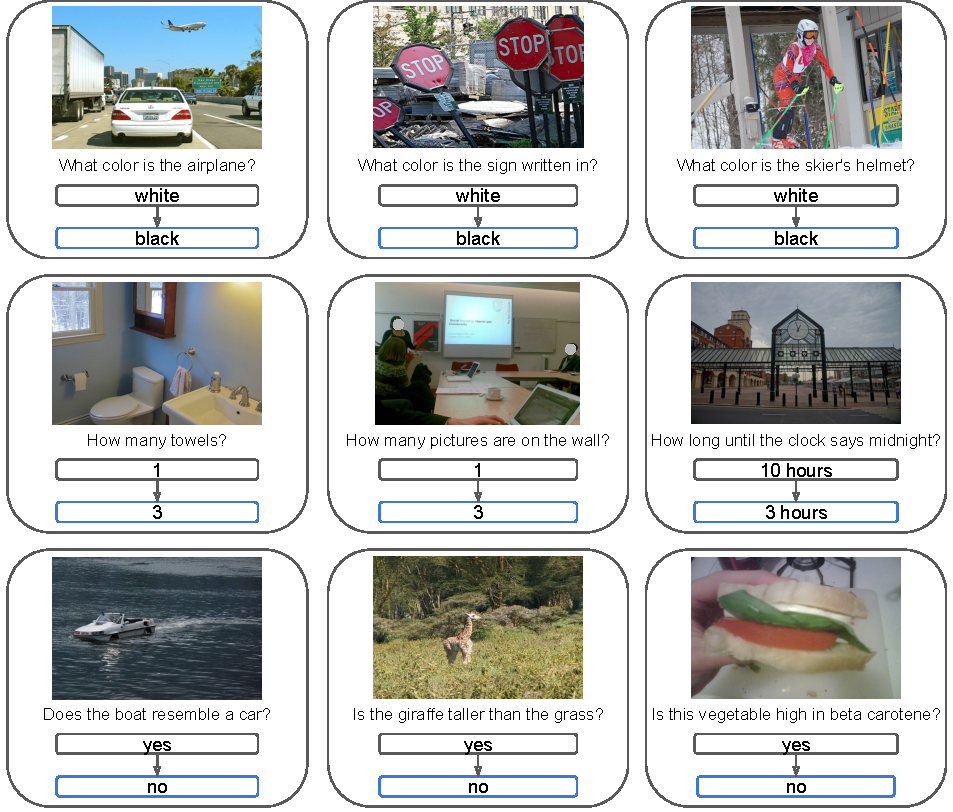
\includegraphics[width=1.0\textwidth]{Figures/model_steering/qualitative/model_steering_change_answers.pdf}
    \end{minipage}%
\caption{\textbf{Steering MLLMs answers.} Each line corresponds to different steering vector that change a specific original answer to a \textcolor{NavyBlue}{target} one. From top to bottom: "white" to "black", "1" to "3" and "yes" to "no".}
\label{fig:app_model_steering_qual_change_answers}
\end{figure*}


\begin{figure*}[t]
    \centering
    \begin{minipage}{\linewidth}
    \centering
        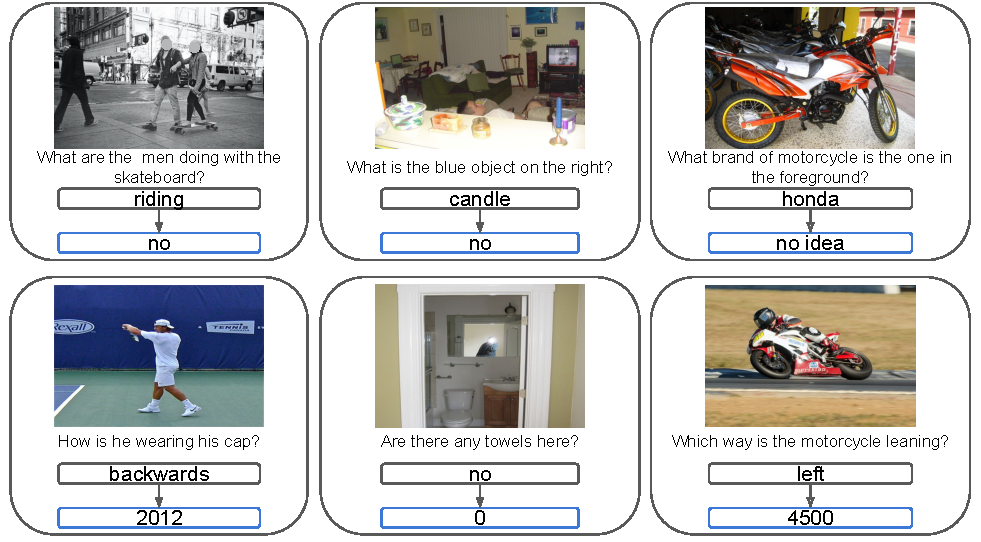
\includegraphics[width=1.0\textwidth]{Figures/model_steering/qualitative/model_steering_change_answers_type.pdf}
    \end{minipage}%
\caption{\textbf{Steering MLLMs answers type.} Each line corresponds to different steering vector that change answers type to a \textcolor{NavyBlue}{target} one. Steering vectors correspond to changing the answers type to yes/no (top) and numbers (bottom).}
\label{fig:model_steering_qual_change_answers_type}
\end{figure*}


\begin{figure*}[t]
    \centering
    \begin{minipage}{\linewidth}
    \centering
        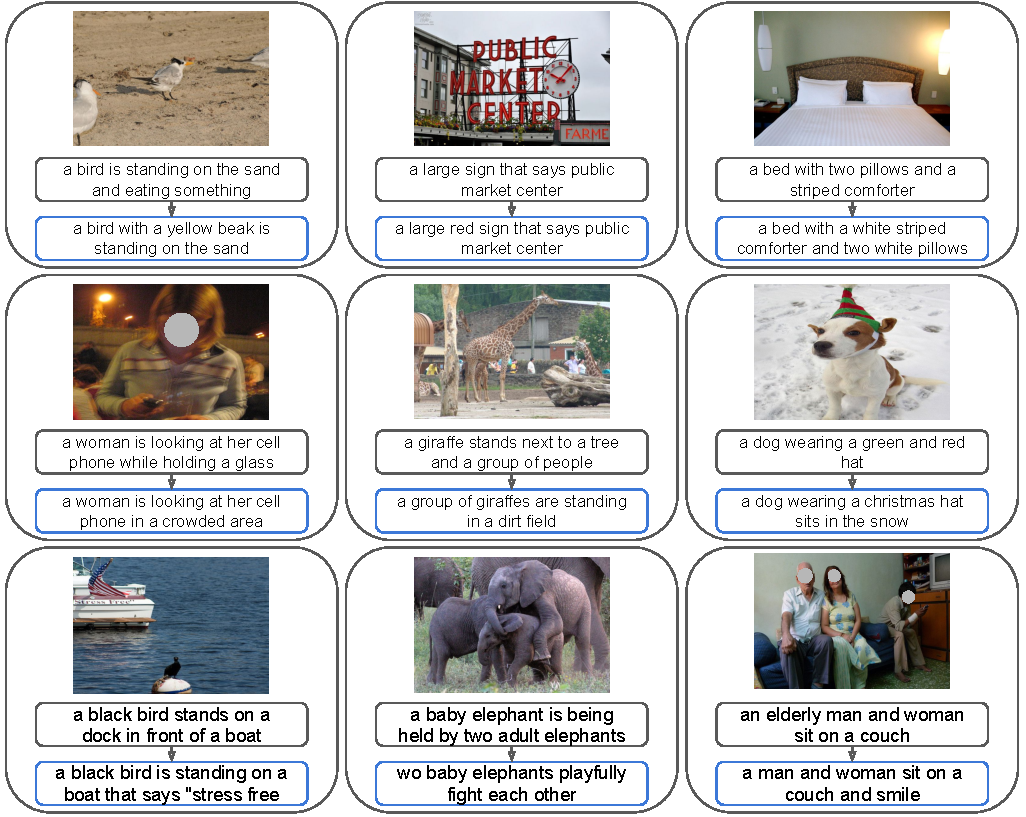
\includegraphics[width=1.0\textwidth]{Figures/model_steering/qualitative/model_steering_change_captions_type.pdf}
    \end{minipage}%
\caption{\textbf{Steering MLLMs captions type.} Each line corresponds to different steering vector that change captions style to a \textcolor{NavyBlue}{target} one. Steering vectors correspond to changing the captions style so that they contain more: colors (top), places (middle) and sentiments (bottom).}
\label{fig:model_steering_qual_change_captions_type}
\end{figure*}



